%                                     MMMMMMMMM        
%                                                                             
%  MMO    MM   MMMMMM  MMMMMMM   MM    MMMMMMMM   MMD   MM  MMMMMMM MMMMMMM   
%  MMM   MMM   MM        MM     ?MMM              MMM$  MM  MM         MM     
%  MMMM 7MMM   MM        MM     MM8M    MMMMMMM   MMMMD MM  MM         MM     
%  MM MMMMMM   MMMMMM    MM    MM  MM             MM MMDMM  MMMMMM     MM     
%  MM  MM MM   MM        MM    MMMMMM             MM  MMMM  MM         MM     
%  MM     MM   MMMMMM    MM   MM    MM            MM   MMM  MMMMMMM    MM
%
%
%            - META-NET Language Whitepaper | Finnish content -
% 
% ----------------------------------------------------------------------------

\begin{document}

\maketitle

\null
\pagestyle{empty} 

\makefundingnotice

\pagenumbering{Roman} 
\setcounter{page}{5}
\pagestyle{scrheadings}

\cleardoublepage

% --------------------------------------------------------------------------
\bsection*{Esipuhe --- Preface}
\begin{Parallel}[c]{78mm}{78mm}
\ParallelLText{\selectlanguage{finnish}
META-NET Valkoiset kirjat -julkaisusarjan tavoitteena on edistää tietämystä
kieliteknologiasta ja sen tarjoamista mahdollisuuksista. Tämä julkaisu
haluaa herättää opettajia, toimittajia, poliitikkoja, kieliyhteisöjä ja
muitakin.

Euroopan kielten kieliteknologisten sovellusten saatavuus vaihtelee. Niinpä
myös toimenpiteet, joita jatkossa tarvitaan tukemaan kieliteknologioiden
tutkimusta ja kehitystä, ovat eri kielten kohdalla 
erilaisia ja riippuvat kielen ominaispiirteistä ja
kieliyhteisön koosta.

Euroopan komission rahoittaman META-NET
-huip\-pu\-osaa\-mis\-ver\-kos\-ton kartoitustyö
kattaa Euroopan 23 virallisen kielen sekä tärkeiden kansallisten ja
paikallisten kielten kieliaineistot ja kieliteknologiat.
Tulosten perusteella kaikkien kartoitettujen kielten
tutkimus kärsii merkittävästä resurssien puutteesta.
Yksityiskohtaisempi nykyisen tilanteen selvitys vahvistaa
tulevan tutkimuksen vaikutusta ja vähentää riskejä.

META-NET koostuu 31 valtion 47 tutkimuskeskuksesta, jotka tekevät
yhteistyötä useiden toimijoiden ja intressiryhmien kanssa. Mukana on
liikeyrityksiä, julkisen hallinnon yksiköitä, teollisuuden edustajia,
tutkimusyksiköitä, tietotekniikan alan yrityksiä, teknologian tuottajia ja
eurooppalaisia yliopistoja. Työn tuloksena on syntymässä teknologinen
visio osana strategista tutkimuslinjausta osoittamaan, miten
kieliteknologiat auttavat Euroopan tutkimusyhteisöä ratkaisemaan
keskeisiä tutkimuskysymyksiä vuoteen 2020 mennessä.
}
\ParallelRText{\selectlanguage{english}
This white paper is part of a series that promotes knowledge about language
technology and its potential. It addresses educators, journalists, politicians,
language communities and others.

The availability and use of language technology in Europe varies between
languages. Consequently, the actions that are required to further support
research and development of language technologies also differ for each
language. The required actions depend on many factors, such as the complexity
of a given language and the size of its community.

META-NET, a Network of Excellence funded by the European Commission, has
conducted an analysis of current language resources and technologies. This
analysis focused on the 23 official European languages as well as other
important national and regional languages in Europe. The results of this
analysis suggest that there are many significant research gaps for each
language. A more detailed expert analysis and assessment of the current
situation will help maximise the impact of additional research and minimise any
risks.

META-NET consists of 47 research centres from 31 countries that are working
with stakeholders from commercial businesses, government agencies, industry,
research organisations, software companies, technology providers and European
universities. Together, they are creating a common technology vision while
developing a strategic research agenda that shows how language technology
applications can address any research gaps by 2020.
}

\ParallelPar
\end{Parallel}
\cleardoublepage

% --------------------------------------------------------------------------
\bsection*{Sisällysluettelo --- Table of Contents}

\renewcommand\contentsname{}
\tableofcontents

\addtocontents{toc}{\protect\thispagestyle{empty}\protect}
\addtocontents{toc}{{\Large\textsf{\centerline{SUOMEN KIELI DIGITAALISELLA AIKAKAUDELLA}}\par}}

\cleardoublepage


% --------------------------------------------------------------------------
\setcounter{page}{1}
\pagenumbering{arabic} 
\pagestyle{scrheadings}


% Start of origin language part
% --------------------------------------------------------------------------


\ssection[Tiivistelmä]{Tiivistelmä}

\selectlanguage{finnish}

\begin{multicols}{2}

Eurooppaan on viimeisen 60 vuoden kuluessa syntynyt selkeä poliittinen
ja taloudellinen, mutta samalla monikulttuurinen ja kielellisesti
moniulotteinen rakenne. Sen kansalaisten tarpeet viestiä keskenään eri
kielillä portugalin kielestä puolaan ja italiasta islantiin, samoin
kuin yritysmaailman ja politiikan sisäinen viestintä, joutuvat siten
väistämättä kohtaamaan kielellisiä esteitä. EU:n instituutioiden
monikielisyyttä säilyttävän politiikan kustannukset, jotka syntyvät
tekstien kääntämisestä ja puhetilanteiden tulkkaamisesta, ovat
vuosittain noin miljardi euroa. Olisiko meillä vaihtoehtoa näin suurelle
taloudelliselle taakalle? Tämän päivän kieliteknologinen ja kielitieteellinen 
tietämys auttaa merkittävällä tavalla monikielisyydestä syntyvien esteiden 
poistamisessa. Kun kieliteknologiaa tulevaisuudessa hyödynnetään älykkäissä
tuotteissa ja sovelluksissa entistä enemmän, voidaan sen avulla
tarjota Euroopan kansalaisille mahdollisuus keskustella ja käydä
kauppaa keskenään vaivattomasti kansallisilla kielillä ilman, että
meidät kaikki pakotetaan hallitsemaan yhtä kaikille yhteistä kieltä.

\boxtext{Kieliteknologia rakentaa yhteyksiä}

Suomalaiset yritykset käyvät entistä enemmän kauppaa Euroopan sisällä.
Tammi-heinäkuussa 2011 Euroopan maiden osuus Suomen tuonnin
kokonaismäärästä oli reilu 77\% ja viennin noin 73\% \cite{SVT}.
Kommunikaation esteet voivat kuitenkin vaikuttaa haitallisesti
kansainväliseen kauppaan, mistä kärsivät erityisesti pienet ja
keskisuuret yritykset, joilla ei ole taloudellisia mahdollisuuksia
vaikuttaa asiaan. Ainoa, joskin kestämättömältä tuntuva vaihtoehto olisi uhrata
Euroopan monikielisyys kaupan alalla ja sallia yhden kielen hallitseva asema ja
hyväksyä riski, että se tulee ajan mittaan korvaamaan kaikki muut
kielet kaupankäynnissä.

Perinteinen tapa ylittää kielellisiä raja-aitoja on opetella vieraita
kieliä. Ilman teknologian apua Euroopan unionin
jäsenvaltioiden 23 virallisen kielen ja lisäksi noin 60 muun eurooppalaisen
kielen hallitseminen käy kuitenkin helposti ylivoimaiseksi. Kielten määrästä
muodostuu este maanosamme kansalaisten ja sen talouden, poliittisen
vuoropuhelun ja tieteellisen kehityksen tielle.

\boxtext{Kieliteknologia avainasemassa}

Ratkaisuksi tilanteeseen ehdotamme keskeisten kieliteknologisten
sovellusten ja teknologioiden kehittämistä vastaamaan viestinnällisiin
tarpeisiin. Ne tulevat tarjoamaan eurooppalaisille toimijoille
merkittäviä etuja, ei ainoastaan Euroopan yhteismarkkina-alueen
sisällä, vaan myös Euroopan ja kolmansien maiden ja erityisesti
niiden nousevien talousmahtien välisissä kauppasuhteissa. Tavoitteen 
saavuttaminen ja Euroopan kulttuurisen monimuotoisuuden säilyttäminen lähtee
liikkeelle siten, että aloitamme kartoittamalla kaikkien Euroopan kielten ominaispiirteitä
sekä selvittämällä, millaista tukea nyt käytettävissä olevat
kielikohtaiset kieliteknologiat niille tarjoavat. Kieliteknologiset
sovellukset tulevat ennen pitkää palvelemaan meitä kaikkia Euroopan 
kielet yhdistävinä rakenteina.

Tavoite on siksi kunnianhimoinen, että sen saavuttaminen nyt tarjolla olevien
automaattisen kääntämisen ja puheen käsittelyn työkalujen avulla näyttää
mahdottomalta. Alan menestyneimmät toimijat ovat pääosin pohjoisamerikkalaisia
yksityisomistuksessa olevia tuottoa tavoittelevia yrityksiä. Euroopan unionissa
ymmärrettiin jo 1970-luvun lopulla kieliteknologian merkitys Euroopan
yhtenäisyyden edistäjänä, ja EU ryhtyi tuolloin rahoittamaan ensimmäisiä omia
tutkimushankkeitaan, esimerkkinä EUROTRA -hanke. Samoihin aikoihin
käynnistettiin kansallisia hankkeita, jotka tuottivat arvokasta tietoa,
mutta eivät kuitenkaan johtaneet yhteiseurooppalaisiin sovelluksiin
käytännössä. Vastakohtana Euroopan valikoivalle rahoituspolitiikalle muut
monikieliset yhteiskunnat kuten Intia (22 virallista kieltä) ja Etelä-Afrikka
(11 virallista kieltä) ovat viime aikoina perustaneet kansallisia pitkän
tähtäimen kieliteknologian tutkimuksen ja teknologisen kehityksen ohjelmia.\\
Alan hallitsevat kieliteknologian toimijat luottavat nykyisin tilastollisiin
lähestymistapoihin, joissa kielen syviä rakenteita analysoivia
kielitieteellisiä menetelmiä tai tietämystä ei juuri hyödynnetä. Esimerkiksi
virkkeitä käännetään automaattisesti vertaamalla tuntematonta virkettä
tuhansiin ihmisen jo kääntämiin virkkeisiin, jolloin tuloksen laatu riippuu
pitkälti käytettävissä olevan verrannaisaineiston määrästä ja laadusta. Jos
kielestä on käytettävissä riittävä määrä aineistoa vertailua varten, voidaan
yksikertaisten virkkeiden automaattisella kääntämisellä päästä käyttökelpoisiin
tuloksiin, mutta pintamuotoihin perustuvat tilastolliset menetelmät ovat
vaikeuksissa sellaisten kielten työstämisessä, joiden käytettävissä olevat
vertailuaineistot ovat hyvin pieniä tai joiden virkerakenne on monimutkainen.\\
Euroopan unioni onkin päättänyt rahoittaa sellaisia hankkeita, kuten EuroMatrix
ja EuroMatrixPlus (vuodesta 2006) sekä iTranslate4 (vuodesta 2010), joissa
tehdään sekä perustutkimusta että soveltavaa tutkimusta ja luodaan resursseja
korkealuokkaisten kieliteknologisten ratkaisujen vakiinnuttamiseksi kaikkiin
eurooppalaisiin kieliin. Kielten syvempien rakenteellisten ominaisuuksien
analyysi on ainoa ratkaisu, kun pyrkimyksemme on tuottaa kaikkien Euroopan
kielten kannalta käyttökelpoisia sovelluksia.\\
Alan eurooppalainen tutkimus on jo saavuttanut tuloksia. Esimerkiksi Euroopan 
unionin käännösyksikkö käyttää nykyisin avoimen lähdekoodin MOSES -konekäännösohjelmistoa, 
joka on suurimmaksi osaksi kehitetty
Euroopan tutkimushankkeiden puitteissa. Sen sijaan, että rakentaisi jo
päättyneiden tutkimusprojektien varaan, Euroopalla on ollut tapana ryhtyä
erillisiin tutkimushankkeisiin, joilla on vähemmän kattava vaikutus
markkinoihin. 
%Oheisyritysten määrä on yksi mahdollinen kriteeri, kun arvioidaan
%aikaisempien hankkeiden taloudellista vaikutusta. Esimerkiksi jo vuonna 1984
%perustettu Trados myytiin Britanniassa toimivalle SDL:lle vuonna 2005.

\boxtext{Kieliteknologia yhdistää Eurooppaa}

META-NETin pitkän tähtäimen tavoite on tuoda korkealuokkaista
kieliteknologiaa kaikkien kielten saataville, jotta poliittinen ja 
taloudellinen yhtenäisyys voidaan saavuttaa kulttuurinen monimuotoisuus
säilyttäen. Teknologia tulee avustamaan olemassa olevien esteiden
poistamisessa ja yhteyksien rakentamisessa Euroopan kielten
välille. Tarvittava teknologinen kehitys edellyttää, että kaikki
toimijat politiikan, tutkimuksen kuin yhteiskunnan saralla yhdistävät
voimansa tavoitteen saavuttamiseksi.\\
Kieliteknologisissa hybridimalleissa kielen syvärakenteen prosessointi
yhdistyy tilastollisiin malleihin. Uskomme niitä hyödyntävän modernin
kieliteknologian mahdollisuuksiin rakentaa yhteyksiä Euroopan kielten
välille. Tässä raportissa kuvataan Euroopan jäsenvaltioiden
kieliteknologian tutkimuksen tilannetta ja kartoitetaan käytettävissä
olevien ratkaisujen valmiusastetta kussakin META-NETin jäsenmaassa.\\
META-NET Valkoiset kirjat -julkaisusarja on hankkeen keskeisiä tehtäviä ja 
se toimii pohjana strategisille toimenpide-ehdotuksille. META-NET julkaisee 
ajantasaista tietoa toiminnastaan, kuten visiopaperin \cite{Vision} ja 
strategisen tutkimussuunnitelman, verkkosivuillaan \url{http://www.meta-net.eu}.


\end{multicols}

\clearpage

\ssection[Uhka kansalliskielille on haaste kieliteknologialle]{Uhka kansalliskielille on haaste kieliteknologialle}
\begin{multicols}{2}

Olemme todistamassa digitaalista vallankumousta, jonka vaikutukset 
viestinnän toimivuuteen ja sitä kautta koko yhteiskuntaan tulevat olemaan merkittäviä. 
Tieto- ja viestintätekniikan viimeaikaista kehitystä on toisinaan verrattu Gutenbergin keksimään
kirjapainotekniikkaan. Millaisia oletuksia Euroopan tietoyhteiskunnan ja erityisesti kieltemme
tulevaisuudesta voimme vertauksen pohjalta tehdä?

\boxtext{Digitaalisen vallankumouksen vaikutukset yhteiskuntaan tulevat olemaan merkittäviä.}	

Gutenbergin keksinnöstä seurasi todellisia läpimurtoja viestinnässä ja tiedon
siirrossa, kuten Lutherin Raamatun käännös kansankielelle. Gutenbergin
ajan jälkeen kuluneina vuosisatoina on kehitetty eri kulttuurien tarpeisiin monenlaisia
teknikoita parantamaan kielenkäsittelyä ja tietämyksen siirtoa:
\begin{itemize}
\item suurten kielten ortografinen ja kieliopillinen standardisointi mahdollisti
\item uusien tieteellisten ja henkisten saavutusten nopean levittämisen;

\item virallisten kielten kehittyminen mahdollisti kansalaisten kommunikoinnin
tiettyjen (usein poliittisten) rajojen sisällä;

\item kielten opetus ja kääntäminen mahdollisti kieltenvälisen viestinnän;

\item tekstin toimittamisen ja bibliografian laatimisen suositusten luominen takasi
painotuotteiden laadun;

\item erilaiset viestintäkanavat, kuten sanomalehti, radio, televisio ja kirja, tyydyttivät erilaisia viestinnällisiä tarpeita.
\end{itemize}
Informaatioteknologia on kuluneiden kahdenkymmenen vuoden aikana auttanut
automatisoimaan asioita ja helpottanut monia toimintojamme arjessa:
\begin{itemize}
\item tietokoneavusteinen julkaisuohjelma on korvannut kirjoituskoneen ja ladonnan;

\item piirtoheitinkalvot tehdään nykyisin esitysmateriaalien
tuottamista varten tehdyillä ohjelmilla, kuten
\foreignlanguage{english}{OpenOfficen} esitysgrafiikat tai Microsoft
PowerPoint;

\item sähköposti lähettää ja vastaanottaa tiedostoja nopeammin kuin faksi;

\item voimme puhua edullisia tai jopa ilmaisia Internet-puheluja ja kokoontua 
virtuaalisesti verkkokeskusteluohjelmien avulla;

\item äänen ja kuvan tallennusformaatit tekevät multimediasisällön jakamisen helpoksi;

\item hakukoneet tarjoavat asiasanaperusteista verkkosivujen hakumahdollisuutta;

\item verkossa olevat palvelut kuten Googlen Kääntäjä tuottavat nopeita, summittaisia
käännöksiä;

\item sosiaalisen median alustat kuten Facebook, Twitter ja Google+ mahdollistavat
kommunikaation, yhteistyön ja tiedonjaon.
\end{itemize}
Vaikka mainitut työkalut ja sovellukset ovat hyödyllisiä, ne eivät vielä kykene
tukemaan kaikkien kansalaisten tavoittamaa monikielistä Euroopan yhteisöä,
jossa tieto ja tavarat voivat liikkua vapaasti.


\subsection{Kielten väliset rajat esteenä Euroopan tietoyhteiskunnan kehitykselle}

Emme kykene ennustamaan tarkasti, millaiselta tulevaisuuden
informaatioyhteiskunta näyttää, mutta on hyvin todennäköistä, että
tietotekniikan vallankumous tuo eri kieliä puhuvia ihmisiä yhteen uusilla
tavoin. Kansalaisille syntyy tarpeita oppia uusia kieliä ja sovellusten
kehittäjille tilaus luoda uusia teknologisia sovelluksia, joiden avulla voidaan 
varmistaa, että ymmärrämme toisiamme ja saavutamme kaiken tarvitsemamme tiedon.
\boxtext{Yhä enemmän kieliä, puhujia ja sisältöä on jatkuvassa vuorovaikutuksessa keskenään.}
Maailmanlaajuisten talousmarkkinoiden alueella ja tiedonkulun kentällä yhä enemmän
kieliä, puhujia ja sisältöä on jatkuvassa vuorovaikutuksessa keskenään uusien
viestintävälineiden avulla entistä nopeammin. Sosiaalisen median (Wikipedia,
Facebook, Twitter, YouTube, ja uusimpana Google+) suuri suosio on vain
jäävuoren huippu.

Voimme nykyisin siirtää gigatavujen kokoisia tekstejä ympäri maailmaa
muutamassa sekunnissa huomaamatta, että toimimme kielellä, jota emme
edes ymmärrä. Euroopan komission tuoreen raportin mukaan 57\%
Internetin käyttäjistä Euroopassa ostaa tavaroita ja palveluja
käyttäen muuta kuin äidinkieltään kaupanteossa. Englanti on kaikkein
tavallisin vieras kieli, ja seuraavina tulevat ranska, saksa ja espanja. 55\%
käyttäjistä lukee sisältöä vieraalla kielellä, kun taas vain 35\%
käyttää vierasta kieltä kirjoittaessaan sähköposteja tai lisätessään
kommentteja verkkoon \cite{EC-prefer}. Vielä muutama vuosi sitten
englannin asema verkon lingua franca -kielenä oli kiistaton — suurin
osa verkossa olevasta sisällöstä oli englanniksi — mutta tilanne on
nyt ratkaisevasti muuttunut. Muilla eurooppalaisilla kielillä samoin
kuin Aasian ja Lähi-idän kielillä tuotetun sisällön määrä on
kasvanut räjähdysmäisesti.

Kielellisten raja-aitojen aiheuttama kuilu sähköisessä kanssakäymisessä  
on saanut hämmästyttävän vähän julkista huomiota. Sen tiedostaminen nostaa kuitenkin
esiin oleellisen kysymyksen: Mitkä Euroopan kielistä  
tulevat kukoistamaan verkottuneessa tieto- ja osaamisyhteiskunnassa, ja mitkä katoamaan?


\subsection{Kielet kohtaavat uusia uhkia}


Samalla kun painotekniikka edisti tiedonvälitystä Euroopan
sisällä, se myös johti monien Euroopan kielten katoamiseen. 
Paikallisilla kielillä ja vähemmistökielillä julkaistiin
harvemmin. Joitakin kieliä, kuten kornin kieli ja dalmatian
kieli, käytettiin vain suullisessa viestinnässä, mikä puolestaan
rajoitti niiden käytön alaa. Tuleeko Internetillä olemaan sama
vaikutus kieleemme?

\boxtext{Euroopan kielten moninaisuus on sen tärkeimpiä voimavaroja.} 
Euroopan noin 80 kieltä muodostavat yhden sen rikkaimmista ja
tärkeimmistä kulttuurien varaan rakentuvista kilpailuvalteista
\cite{EC-multi}. Vaikka isot kielet, kuten englanti ja espanja, tulevat
todennäköisesti selviytymään kasvavilla digitaalisilla markkinoilla,
voivat monet eurooppalaisista kielistä joutua verkostoituneessa
yhteiskunnassa yhdentekevän kielen asemaan. Tällainen kehitys
heikentäisi Euroopan asemaa maailmassa ja haittaisi Euroopan
strategiaan sisältyvää tavoitetta taata kaikille Euroopan kansalaisille
yhtäläinen oikeus osallistumiseen kielestä riippumatta. 
Unescon raportti monikielisyydestä osoittaa, että kielet
ovat elintärkeitä perusoikeuksien turvaamisessa, joita ovat
esimerkiksi oikeus koulutukseen, oikeus ilmaista poliittinen mielipiteensä 
ja oikeus osallistua yhteiskunnalliseen toimintaan \cite{UN-mid}.


\subsection{Kieliteknologia tukee kielten säilymistä}


Tähän asti toimenpiteet kielen säilymisen puolesta ovat kohdistuneet lähinnä kielen
opetukseen ja kääntämiseen. Eurooppalaiset käännöstoiminnan, tulkkauksen 
ja lokalisoinnin markkinat vuonna 2008
olivat 8,4 miljardin euron arvoiset ja niiden odotetaan yhä kasvavan
10 prosentin vuosivauhdilla \cite{EC-size}. Luku kattaa kuitenkin vain
pienen osan kieltenvälisen viestinnän nykyisistä ja tulevaisuuden
tarpeista. Tavoitteena on varmistaa, että tulevaisuuden Euroopassa
kansallisia kieliä voidaan käyttää laaja-alaisesti kaikkiin
tarkoituksiin. Tarkoituksenmukainen teknologia on avuksi tavoitteen 
saavuttamisessa samalla tavoin kuin teknologia ratkaisee mm. kuljetuksen ja 
energiatalouden kysymyksiä ja vastaa erityisryhmien tarpeisiin.
\boxtext{Kieliteknologiat auttavat meitä ottamaan osaa monikieliseen 
sosiaaliseen ja poliittiseen keskusteluun.}
Kieliteknologian tutkimuskohteita ovat kaikki kirjoitetun ja puhutun kielen
muodot. Sovellukset auttavat meitä tekemään yhteistyötä, hoitamaan
liikeasioita, jakamaan tietoa ja ottamaan osaa sosiaaliseen ja poliittiseen
keskusteluun kielellisistä rajoitteista ja tietotekniikan taidoista
riippumatta. Usein ne toimivat apunamme näkymättömällä tavalla monimutkaisten
tietokonejärjestelmien syvyyksissä ja auttavat:
\begin{itemize}
\item löytämään tietoa Internetin hakukoneen avulla;

\item tarkistamaan tekstinkäsittelyohjelman sisällä oikeinkirjoituksen ja kieliopin;

\item saamaan tuotetta koskevia suosituksia näkyviin verkkokaupassa;

\item kuuntelemaan puhuttua ohjeistusta auton navigaattorista;

\item kääntämään verkkosivuja verkossa olevan palvelun avulla.
\end{itemize}

Kieliteknologiat koostuvat erilaisista keskeisistä ydinteknologioista, joita
käytetään laajemmissa tehtäväkokonaisuuksissa monenlaisten tehtävien
suorittamiseen. Tavoitteena META-NET valkoisten kirjojen julkaisusarjassa on 
selvittää, missä vaiheessa eurooppalaisten kielten ydinteknologiat tänään ovat.

\boxtext{Eurooppa tarvitsee vakaata, kohtuuhintaista 
ja tärkeimpiin ohjelmistoympäristöihin integroitua kieliteknologiaa.}
Jotta voisimme säilyttää asemamme kehityksen etujoukoissa maailmassa,
tarvitsemme kaikille Euroopan kielille sovitettua kieliteknologiaa, joka on
vakaata, kohtuuhintaista ja tärkeimpiin ohjelmistoympäristöihin tiiviisti
integroitua. Ilman kieliteknologiaa emme pääse käyttäjinä nauttimaan todella
tehokkaista, interaktiivisista ja multimediaa tehokkaasti hyödyntävistä
monikielisistä sovelluksista lähitulevaisuudessa.



\subsection{Kieliteknologian mahdollisuuksia}


Painotuotteiden maailmassa todellinen teknologinen läpimurto oli paperilla
olevan kuvan (tekstin) nopea monistaminen käyettävissä olevalla tekniikalla toimivan
kirjapainokoneen avulla. Ihmisten piti noina aikoina tehdä tiedon etsimisen,
omaksumisen, kääntämisen ja tiivistämisen edellyttämä työ käsityönä. Puheen
nauhoittamiseksi piti odottaa Edisonia – ja silloinkin tuloksena oli
vain analogisia kopioita.\\
Nykyisin kieliteknologia tarjoaa mahdollisuuden automatisoida kääntämisen,
sisällöntuotannon ja tietämyksen hallinnan prosesseja kaikilla Euroopan
kielillä. Sitä tarvitaan myös mahdollistamaan helppokäyttöisiä kieleen tai
puheeseen pohjautuvia käyttöliittymiä kotitalouksille suunnattuihin
elektronisiin tuotteisiin, ajoneuvoihin, tietokoneisiin ja robotteihin. Vaikka
kaupalliset ja teolliset sovellukset ovat todellisuudessa vielä kehityksen
esiasteita, tutkimuksen ja tuotekehityksen saavutukset luovat aitoja
mahdollisuuksia tulevaisuuden ratkaisuihin. Erikoisalojen konekäännös toimii
esimerkiksi jo suhteellisen tarkasti, ja kokeelliset sovellukset sisältävät
monikielisiä informaation ja tietämyksen hallintatyökaluja samoin kuin
sisällöntuotantoa tukevia ohjelmia useilla eurooppalaisilla kielillä.\\
\boxtext{Kieliteknologia auttaa vastaamaan monikielisyyden haasteisiin.}
Useimpien teknologioiden tavoin ensimmäiset kieliteknologiset sovellukset,
kuten äänipohjaiset käyttöliittymät ja dialogijärjestelmät, kehitettiin hyvin
erikoistuneille aloille ja niiden suorituskyky on usein rajallinen. Toisaalta
opettamisen puolella ja viihdeteollisuudessa löytyy huikeita kaupallisia
mahdollisuuksia integroida kieliteknologioita peleihin,
kulttuuriperintösivustoihin, opetusviihdepaketteihin, kirjastojen palveluihin, erilaisiin 
simulaatioympäristöihin ja harjoitteluohjelmiin. Mobiilit tietopalvelut,
tietokoneavusteinen kielen oppiminen, verkko-opetusympäristöt, itsearvioinnin
työkalut ja plagioinnin tunnistusohjelmat ovat vain joitakin esimerkkejä
sovellusaloista, joissa kieliteknologialla voi olla tärkeä rooli. Sosiaalisen
median sovellusten kuten Twitterin tai Facebookin suosio osoittaa, että
jatkossakin tarvitaan kehittyneitä kieliteknologioita, joiden avulla voidaan
tarkkailla viestiliikennettä, tehdä yhteenvetoja keskusteluista, havaita
trendejä erilaisten kyselyjen perusteella, dokumentoida tunnepohjaisia reaktioita tai tunnistaa 
tekijänoikeusloukkauksia.\\
Kieliteknologia tarjoaa Euroopan unionille monenlaisia ratkaisuja. Se auttaa
meitä vastaamaan Euroopan moninaisiin monikielisyyden haasteisiin – siihen
arkipäivään, jossa eri kielet elävät luonnostaan sovussa eurooppalaisessa
liike-elämässä, organisaatioissa ja kouluissa. Mutta kansalaisten tulee voida
kommunikoida ristiin rastiin Euroopan yhteismarkkina-alueella kielten rajojen
yli - ja tätä kieliteknologia voi edesauttaa tarjoamalla ratkaisuja, jotka ovat
kaikkien kansalaisten saavutettavissa ja joiden avulla kommunikointi
onnistuu kaikilla kielillä. Kieliteknologia voidaan nähdä avustavana
teknologiana, kun ratkaistaan kielellisen monimuotoisuuden kysymyksiä ja
helpotetaan kieliyhteisöjen välistä viestintää. Eräs aktiivisista tutkimuskohteista 
on kieliteknologian hyödyntäminen pelastusoperaatioissa katastrofialueilla, 
kun toimintakyvyn ripeys on elämän ja kuoleman kysymys: tulevaisuuden useita 
kieliä taitavat älykkäät koneet voivat pelastaa ihmishenkiä.\\
Panostamalla tulevaisuudessa innovatiiviseen eurooppalaiseen monikieliseen
kieliteknologiaan Eurooppa voi näyttää suuntaa muulle maailmalle.



\subsection{Kieliteknologian haasteita}


Vaikka kieliteknologia on tutkimus- ja sovellusalueena jo ottanut isoja
edistysaskeleita, on teknologinen edistys ja tuotekehitys nykyisellään liian
hidasta. Laajalti käytössä olevat teknologiat, kuten oikeinkirjoituksen ja
kieliopin tarkistusohjelmat, ovat tyypillisesti yksikielisiä ja niitä on
saatavissa vain kouralliselle kieliä. Verkon tarjoamat käännöspalvelut, vaikka
ovatkin hyvä apu tiedoston sisällön likimääräisen vastineen tuottamisessa,
ovat hankaluuksissa heti, kun tarvitaan oikein tarkkoja ja yhdenmukaisia
käännöksiä. Ihmiskielen monimutkaisuudesta johtuen kielten mallintaminen
ohjelmallisesti ja niiden testaaminen todellisessa elämässä on pitkä ja kallis
liiketoiminnan muoto, joka edellyttää pitkän aikavälin rahoitussitoumuksia.
\boxtext{Teknologinen edistys ja tuotekehitys tapahtuvat liian hitaasti.}
Euroopan tulee siksi pitää kiinni edelläkävijän roolistaan monikielisen
yhteisön teknologisten haasteiden kohtaamisessa ja kehittää uusia menetelmiä
kehityksen nopeuttamiseksi koko Euroopassa. Nämä voivat tarkoittaa sekä
tietoteknisiä edistysaskeleita että uusia tekniikoita, kuten yleisön
osallistamisen menetelmä kansalaisten tietämyksen hyödyntämisessä.



\subsection{Kielen omaksumisesta}


Ennen kuin lähdemme pohtimaan tarkemmin sitä, miten tietokoneet käsittelevät
kieliainesta ja miksi niitä on vaikeaa ohjelmoida hyödyntämään kieltä,
tarkastelemme lyhyesti ihmisten ensimmäisen ja toisen kielen omaksumista ja sen
jälkeen tutustumme tarkemmin kieliteknologisten järjestelmien toimintaan.
Ihmiset oppivat kieltä kahdella tavalla, oppimalla esimerkeistä ja
tekemällä niistä yleistyksiä.  Vauvat omaksuvat kielen kuuntelemalla
ja osallistumalla itse aitoihin vuorovaikutustilanteisiin
vanhempiensa, sisarustensa ja muiden perheenjäsenten kanssa. Noin
kaksivuotiaista eteenpäin lapset alkavat tuottaa sanoja ja lyhyitä
fraaseja itse. Tämä on mahdollista ainoastaan siksi, että ihmisillä on
geneettinen taipumus matkimiseen ja kuulemansa puheen analysointiin.
\boxtext{Ihmiset oppivat kieltä kahdella tavalla, oppimalla esimerkeistä ja tekemällä niistä yleistyksiä.}
Vanhempana lapsen vieraan kielen oppiminen vaatii enemmän vaivannäköä, pääosin
siksi, että oppija ei enää ole osa kieltä äidinkielenään puhuvien kieliyhteisöä.
Koulussa vieraat kielet usein omaksutaan opettelemalla kielen kieliopillista
rakennetta, sanastoa ja oikeinkirjoitusta harjoitusten avulla, jotka kuvaavat
käsitystämme kyseisestä kielestä abstraktien sääntöjen, taulukoiden ja
esimerkkien kautta. Vieraan kielen oppiminen vaikeutuu iän myötä.
Kieliteknologisten menetelmien kaksi päätyyppiä oppivat tietoa kielestä samalla
tavoin. Tilastolliset (tai ‘aineistolähtöiset’) lähestymistavat eristävät
kielitietoa valtavista aitojen esimerkkitekstien kokoelmista. Vaikka
esimerkiksi oikeinkirjoituksen tarkistimelle riittää harjoitusaineisoksi yksikielinen teksti, 
konekäännösjärjestelmien treenaamiseen tarvitaan
rinnakkaistekstejä kahdesta tai useammasta kielestä. Konekäännösalgoritmi oppii
niiden rakenteita ja päättelee, miten sanat, lyhyet fraasit ja kokonaiset virkkeet on
niissä käännetty.
\boxtext{Kieliteknologisten menetelmien päätyypit oppivat tietoa kielestä samalla tavoin.}

Tilastollinen lähestymistapa saattaa edellyttää miljoonien virkkeiden
aineistoa, ja menetelmien laatu paranee analysoidun tekstin määrän kasvaessa.
Tämä on yksi syy siihen, että hakukoneiden kehittäjät keräävät niin suuria
määriä kirjoitettua kieliainesta kuin mahdollista. Google-haku ja Googlen
Kääntäjä perustuvat kaikki tilastollisiin menetelmiin. Tilastoista saatava
suuri hyöty syntyy koneen kyvystä oppia nopeasti sille jaksoittaisena
tarjotusta harjoitusaineksesta, vaikkakin oppimistulosten laatu voi vaihdella.\\
Toinen kieliteknologian ja erityisesti konekääntämisen lähestymistapa on
sääntöpohjaisten järjestelmien rakentaminen. Kielitieteen,
tietokonelingvistiikan ja tietojenkäsittelytieteen asiantuntijat koodaavat
aluksi kieliopillisia analyysejä (kääntämisen sääntöjä) ja kokoavat sanastoja
(leksikkoja). Jotkin johtavista sääntöpohjaisista konekäännösjärjestelmistä
ovat olleet tekeillä jo yli kaksikymmentä vuotta. Sääntöpohjaisten
järjestelmien suuri etu piilee siinä, että asiantuntijat voivat kontrolloida
kielen prosessointia tarkemmin. Näin heidän on mahdollista korjata ohjelman
virheitä systemaattisesti ja antaa yksityiskohtaista palautetta käyttäjälle,
erityisesti tilanteessa jossa sääntöpohjaisia järjestelmiä käytetään kielen
oppimisessa. Mutta työn kalleudesta johtuen on sääntöpohjaisia
kieliteknologisia menetelmiä tähän asti kehitetty vain isoille kielille.\\
Koska tilastollisten ja sääntöpohjaisten järjestelmien vahvuudet ja heikkoudet
tapaavat olla toisiaan täydentäviä, tutkimushankkeissa keskitytään molemmat
menetelmät yhdistäviin hybridimalleihin. Näiden osalta menestystä on
toistaiseksi koettu enemmän tutkimuslaboratoriossa kuin teollisten sovellusten
maailmassa.\\
Kuten olemme tässä osiossa nähneet, monet nykyisessä informaatioyhteiskunnassa
hyödynnettävät sovellukset perustuvat kieliteknologisiin menetelmiin. Tämä on
erityisen tyypillistä Euroopan monikieliselle talousmarkkinoiden ja tiedonjaon
alueelle. Vaikka kieliteknologian parissa on viime vuosina saavutettu
merkittäviä edistysaskeleita, on kieliteknologisten järjestelmien laadullisessa
parantamisessa vielä valtavasti työtä ja mahdollisuuksia. Seuraavissa osioissa
tarkastellaan suomen kielen roolia eurooppalaisessa tietoyhteiskunnassa ja
arvioidaan kieliteknologian tämänhetkistä tilaa suomen kielen näkökulmasta.


\end{multicols}
\clearpage
\ssection[Suomen kieli Euroopan tietoyhteiskunnassa]{Suomen kieli Euroopan tietoyhteiskunnassa}

\begin{multicols}{2}
\subsection{Perustietoa suomen kielen asemasta ja käytöstä}



Suomen kieltä puhuu äidinkielenään Suomessa noin 4,8 miljoonaa ihmistä, ja
se on noin 0,5 miljoonan suomalaisen toinen kieli. Suomea puhutaan myös
Ruotsissa, Virossa, Venäjällä, Yhdysvalloissa ja Australiassa.

\boxtext{Suomen kieli on yksi Euroopan unionin virallisista kielistä}
Suomen perustuslain ja kielilain mukaan suomi on ruotsin ohella Suomen toinen
kansalliskieli. Lisäksi suomi on Ruotsin virallinen vähemmistökieli (vuonna 
2011 lähinnä Pohjois- ja Keski-Ruotsin kunnissa). Suomen kieli on yksi 
Euroopan unionin virallisista kielistä. Suomen ja ruotsin lisäksi
Suomessa on vanhastaan käytetty kolmea saamen kieltä, pohjoissaamea,
inarinsaamea ja koltansaamea, Suomen romanikieltä, karjalan kieltä ja kahta
viittomakieltä. Lähinnä 1800-luvulta lähtien Suomessa on asunut myös venäjän-
ja tataarinkielisiä. 1970-luvun lopun jälkeen Suomeen on muuttanut väestöä
muualta Euroopasta, Aasiasta ja Afrikasta, ja maahanmuuttajakieliä on nykyisin
runsaat 100 kieltä. Suurimmat ryhmät ovat venäjän-, viron- ja somalinkielisiä.\\
Suomen kirjakielellä on suhteellisen lyhyt historia. Hengellisen kirjallisuuden
ja kirkon kielenä suomea on käytetty 1500-luvulta lähtien, lain kielenä
1700-luvulta lähtien. Hallinnon, opetuksen ja kirjallisuuden kielenä oli aina
1800-luvulle ruotsi. Nykysuomelle luotiin perusta 1800-luvulla, jolloin suomen
kielestä tuli täysivaltainen kieli kaikessa yhteiskunnallisessa toiminnassa.\\
Suomen murteet jakautuvat kahteen pääryhmään, länsimurteisiin ja itämurteisiin.
Länsimurteita ovat lounaismurteet, lounaiset välimurteet, hämäläismurteet,
Etelä-Pohjanmaan murre, keski- ja pohjoispohjalaiset murteet ja Peräpohjan
murteet. Itämurteita ovat savolaismurteet ja kaakkoismurteet. Murteet eroavat
toisistaan äänne- ja muotopiirteiltään (idässä \textit{meijän}, \textit{männä}, lännessä \textit{meirän},
\textit{mennä}) ja osin sanastoltaan (idässä \textit{vasta}, lännessä \textit{vihta}). Murre-erot ovat
edelleenkin selviä, ja varsinkin intonaatio erottaa eri alueiden puhujat
erottuvat toisistaan varsinkin puheen prosodiaan (mm. intonaatioon tai
ajoitukseen) liittyvien piirteiden perusteella. Erot ovat kuitenkin sellaisia,
että erimurteiset ymmärtävät toisiaan hyvin. Kaupungistuminen ja yhteiskunnan
muut muutokset ovat tasoittaneet murteita niin, että kaikkein suppea-alaisimmat
ja leimallisimmat variantit ovat hävinneet.


\subsection{Suomen kielen erityispiirteitä}

Suomen kieli kuuluu suomalais-ugrilaisten kielten ryhmään, ja se on yksi
itämerensuomalaisista kielistä. Muut itämerensuomalaiset kielet ovat karjala,
lyydi, vepsä, inkeroinen, vatja, viro, liivi, võro ja seto. Näissä kielissä ei
ole kieliopillista sukua eikä artikkeleita.\\
Suomen kielen leimallisimpia piirteitä on, että kirjoitus pääosin vastaa
ääntöasua. Sanan pääpaino on ensimmäisellä tavulla.\\
Suomen kielen ominaispiirteitä on rikas taivutusjärjestelmä. Sanat jakautuvat
kolmeen pääryhmään: Nomineilla on sija- ja lukutaivutus, ja adjektiivit
kongruoivat pääsanansa kanssa (\textit{isossa talossa}, \textit{isoissa taloissa}), verbeillä on
persoona-, tempus- ja modustaivutus (\textit{sanon}, \textit{sanot}, \textit{hän sanoo}, \textit{sanomme}, \textit{sanotte},
\textit{he sanovat}; \textit{sanon}, \textit{sanoin}, \textit{olen sanonut}, \textit{olin sanonut}; \textit{sanon}, \textit{sanoisin}) ja
adpositiot, adverbit ja partikkelit ovat pääosin taipumattomia. Sijoja on 15,
joista akkusatiivi esiintyy vain persoonapronomineissa ja \textit{kuka}-pronominissa (\textit{minut}, \textit{meidät}, \textit{kenet}).
\boxtext{Suomen kielessä on rikas taivutusjärjestelmä.}

Nomineilla voi olla jopa 2 000 ja verbeillä yli 12 000 taivutusmuotoa.
Erilaisten muotojen määrä johtuu suomen agglutinatiivisesta luonteesta: sanaan
voidaan liimata suuri joukko taivutuspäätteitä ja muita affikseja, esimerkiksi
\textit{halu}+\textit{tu}+\textit{imm}+\textit{i}+\textit{lla}+\textit{mme}+\textit{ko}.

Tärkeimmät suomen kielen sananmuodostuskeinot ovat johtaminen eli derivaatio ja
yhdistäminen eli kompositio. Sanakirjojen hakusanoista perussanoja on noin
10–15 \%, johdoksia noin 20–30 \% ja yhdyssanoja noin 60–70 \%.
\begin{itemize}
\item Johdoksia: \textit{kirja $\to$ kirjasto, kirjaamo, kirjallisuus, kirjoittaa, kirjanen,
    kirjallinen} jne.

\item Yhdyssanoja: \textit{maahanmuutto, kansaneläkelaitos, yleisurheilumaaottelu.}
\end{itemize}
Päätteiden kasautumisen lisäksi suomen kielelle ominaisia piirteitä ovat
astevaihtelu ja vokaaliharmonia. Taivutuspäätteiden lisäksi sanoista tekee
pitkiä yhdyssanojen kirjoittaminen yhdeksi sanaksi ilman välilyöntejä tai
yhdysmerkkejä. Yhdyssanoista voi lisäksi edelleen muodostaa uusia yhdyssanoja.

\boxtext{Suomen erityispiirteet ovat kieliteknologian kannalta haasteellisia.}
Lauseenjäsenten yleisin järjestys on tyyppiä SVX, \textit{Hän osti polkupyörän}. Suomen
sanajärjestys vaihtelee kuitenkin sen mukaan, mikä on lauseen
informaatiorakenne, eli sanajärjestyksellä osoitetaan tutun ja uuden tiedon
suhdetta:
\begin{itemize}
\item \textit{Hän osasi läksynsä.}

\item \textit{Osasi hän läksynsä.}
\end{itemize}

Syntaktisia rooleja merkitään taivutuspäätteiden avulla. Siksi suomen
sanajärjestys on suhteellisen vapaa, toisin sanoen tekijä ja tekemisen kohde
tunnistetaan ensisijaisesti taivutuspäätteen perusteella:
\begin{itemize}
\item \textit{Poika osti kirjan.}

\item \textit{Kirjan poika osti.}
\end{itemize}



\subsection{Suomen kielen kehityksestä}


Suomen kirjakielen historia on suhteellisen lyhyt. Ensimmäiset suomenkieliset
tekstit olivat saksan kielestä uuden aikakauden alkupuolella suomeen
käännettyjä uskonnollisia tekstejä. Kirjoitusasu alkoi kuitenkin vakiintua
vasta 1800-luvulla. Toisen maailmansodan aikana suomen kieleen lainattiin
sanoja pääasiassa ruotsista, saksasta ja latinasta. Nykyisin sanastossamme on
vain pieni suomalais-ugrilaista alkuperää oleva osuus.\\
Suomen kielessä on runsaasti lainasanoja eri ajoilta, balttilaisia,
germaanisia, slaavilaisia ja skandinaavisia lainasanoja. Vuosisatojen
ajan vahva lainanantajakieli oli ruotsi (\textit{pankki} <
\textit{bank}, \textit{laki} < \textit{lag}, \textit{treenata} <
\textit{träna} ). Nykyisin lainoja omaksutaan lähinnä englannista
(\textit{liisaus} < \textit{leasing}, \textit{meili} < \textit{mail}),
erikoiskieliin myös muualta (\textit{pitsa},
\textit{karate}). Tyypillistä on, että useimmat lainasanat mukautuvat
varsin nopeasti suomen kielen rakenteeseen ja
taivutusjärjestelmään. Lainasanat ja omaperäiset sanat elävät usein
rinnan: \textit{tulostin} $\sim$ \textit{printteri}.\\
Viime aikoina on ollut nähtävissä myös englannin kielen toisenlainen vaikutus.
Suomen kielen käyttöala on eräillä elämänalueilla kapeutunut, eikä suomea
käytetä siinä määrin kuin ennen. Tämä ilmiö näkyy selvimmin luonnontieteessä ja
tekniikassa, mutta myös muualla tiedeyhteisössä. Tiedeyhteisö on myös entistä
tietoisempi siitä, että suomen kieli vaatii enemmän huomiota kuin viime
vuosikymmeninä.\\
Puhutun ja kirjoitetun kielen suhde on myös muutoksessa. Nykyisin julkaistaan
paljon verkossa sellaista tekstiä, joka on oikeastaan puhetta. Siksi puhekielen
ilmiöt tulevat mukaan kirjoitettuun kieleen voimallisemmin kuin aiemmin.\\
Suomen kielen virallinen huolto on lain ja asetuksen mukaan Kotimaisten kielten
keskuksen tehtävä.


\subsection{Suomen kielen huolto}

Suomen kielen virallinen huolto on lain ja asetuksen mukaan Kotimaisten kielten
keskuksen tehtävä. Tutkimuskeskus antaa suosituksia, opastaa, kouluttaa
sekä kartuttaa ja pitää yllä ajantasaisia suomen kielen tietokantoja.
Neuvonnalla on pitkä perinne, ja toiminta tunnetaan hyvin kansalaisten
keskuudessa. Suomalainen kielenhuolto on yhä enemmän tekstinhuoltoa, vaikka
oikeinkirjoituksen ja taivutuksen yksityiskohdatkin ovat kyllä kysymysten
kohteena.
\boxtext{Suomen kielen huolto kuuluu KOTUKSEN tehtäviin.}

Suomenkielisen termityön keskeisiä kehittäjiä on Sanastokeskus TSK, ja
termityötä tehdään myös monissa tieteellisissä seuroissa. Vuoden 2011 alussa
käynnistyi Helsingin yliopistossa hanke Tieteen kansallinen termipankki, jonka
tarkoituksena on edistää suomenkielisten tieteellisten termien laatimista ja
niiden saamista laajaan käyttöön.\\
2000-luvulla on yhä enemmän alettu kiinnittää huomiota myös viranomaiskielen
laatuun ja ymmärrettävyyteen. Kotimaisten kielten keskus on tehnyt
poliitikoille monia aloitteita virkakielen parantamiseksi ja tekee läheistä
yhteistyötä lainlaatijoiden kanssa.


\subsection{Kieli ja oppiminen}


 
Noin 56 000 lasta aloittaa vuosittain koulunkäyntinsä suomalaisessa
peruskoulussa integroidussa yhdeksänvuotisessa koulujärjestelmässä. Suomen
kielellä on tärkeä asema kaikkien vuosikurssien opetussuunnitelmassa, jossa
määritellään opetustuntien kokonaismäärä. Opetuksen jakautumisesta eri
vuosiluokkien osalle voidaan sitten päättää paikallisesti. Peruskoulun yhdeksän vuoden
kuluessa oppilaat osallistuvat yhteensä 1554 äidinkielen ja kirjallisuuden oppitunnille.
\boxtext{Suomi on menestynyt kaikilla PISA-arviointikierroksilla.}
Suomi on osallistunut kaikille neljälle PISA-arviointikierrokselle
vuosina 2000, 2003, 2006 ja 2009. Testitulokset osoittavat, että
perusopetus on ollut suomalainen menestystarina siitäkin huolimatta,
että erot tyttöjen ja poikien suoritustasoissa ovat PISA-arvioihin
osallistuneiden maiden suurimmat \cite{Literacy}. Vuonna 2009 lukutaito 
oli arvioinnin keskeinen osa-alue, ja suomalaisten oppilaiden
suoritusten keskiarvo arvioitiin edellisten PISA-kierrosten tavoin
kolmanneksi parhaaksi. Lukutaito oli tuolloin arvioinnin keskeinen osa-alue, 
ja suomalaisten oppilaiden suoritusten keskiarvo
arvioitiin edellisten PISA-kierrosten tavoin kolmanneksi parhaaksi
\cite{Pisa2006}. Lukemista tuetaan myös muilla keinoin,
esimerkiksi tiheä kirjastoverkosto ja suuri valikoima lehtiä on
tarjolla kaikille ikäluokille.\\
Lukiossa opiskelijat osallistuvat kuudelle pakolliselle
äidinkielen ja kirjallisuuden kurssille ja voivat lisäksi
halutessaan valita kolme ylimääräistä syventävää kurssia. Äidinkieli
on pakollinen oppiaine ylioppilaskirjoituksissa, joiden jälkeen
opiskelijat voivat hakeutua korkean asteen opintoihin muun muassa
käytäntöön painottuviin ammattikorkeakouluihin tai teoreettisempiin
yliopisto-opintoihin. Vuosittain aloituspaikan ammattikorkeakoulusta
saa noin 36 000 opiskelijaa ja noin 20 000 aloittaa yliopistoissa
\cite{Education}. Kaikkien 26 ammattikorkeakoulun ja 16 yliopiston
opetusohjelmat sisältävät pakollisia äidinkielen opintoja.\\
Suomalaiset oppilaat opiskelevat äidinkieltään peruskoulun yläasteella
vähemmän kuin OECD-maiden oppilaat keskimäärin, eikä äidinkielen tai
kirjallisuuden ylimääräisten kurssien valitseminen ole 
erityisen suosittua, vaikka oppiainetta pidetään tärkeänä. Raportin
\textit{Suomen kielen tulevaisuus} \cite{Tulevaisuus2009} työryhmä
ehdottaakin, että kurssivalikoiman tulisi myös sisältää myös muita
kuin tekstin tuottamisen tai kirjallisuuteen painottuvia kursseja,
kuten kielitieteellisiä opintoja.\\
Suomen kieltä voi opiskella pääaineena kahdeksassa Suomen viidestätoista
yliopistosta (Helsingin, Jyväskylän, Oulun, Tampereen, Turun, Vaasan
ja Itä-Suomen yliopistoissa sekä Åbo Akademissa) ja Suomen kirjallisuutta
kuudessa ensimmäisessä \cite{hum-ulko}. Yksittäisiä kursseja on mahdollista 
opiskella monissa muissakin yliopistoissa. Englannin merkitys opetuskielenä on
lisääntynyt samassa tahdissa kansainvälisen opiskelija-aineksen määrän
kasvun kanssa, mutta suomi on vielä pääasiallinen opetuskieli
useimmissa tutkinto-ohjelmissa \cite{Board}.



\subsection{Kansainvälisiä näkökulmia}

Suomen kieli on 1900-luvun lopulle asti ollut kansainvälisissä
yhteyksissä vastaanottava kieli. Maailman kaunokirjallisuus ja tieteen
saavutukset on saatu Suomeen käännösten välityksellä. Myös
populaarikulttuurin, esimerkiksi musiikin sanoitusten, kääntämisellä
on ollut vahva asema 1990-luvulle asti. Näin Suomeen on syntynyt vahva
kääntämisen perinne ja tottumus lukea ja kuulla käännettyä
kieltä. Tässä suhteessa on kuitenkin viime vuosikymmeninä tapahtunut
muutosta, koska Internet-yhteydet ovat moninkertaistaneet
muunkielisten tekstien ja muiden kulttuurin tuotteiden käytön;
tavallisin vieras kieli on silloin englanti.
\boxtext{Suomen kieli on ollut kansainvälisissä yhteyksissä vastaanottava kieli.}

Kääntäminen suomesta muihin kieliin on myös ollut
tärkeää. Elinkeinoelämän ja tieteen kansainvälisissä kontakteissa taas
suomi on ollut käännösten lähtökieli, sillä yhteyksiä ei yleensä ole
voitu hoitaa suomen kielellä. Suomen kieltä voi tosin opiskella
useissa maailman yliopistoissa, mutta opiskelijamäärät ovat pieniä ja
useimmilla opiskelijoilla on enemmänkin sukujuuriin tai
henkilökohtaisiin suhteisiin kuin ammattiin liittyvät syyt
opiskeluunsa. Kansainvälisten kontaktien jokapäiväistyminen on
muuttanut myös suomesta kääntämisen tilannetta, sillä yhä useammat
suomalaiset kirjoittavat itse muilla kielillä, tavallisimmin
englanniksi. Muutama suomalainen suuryritys on ottanut
konsernikielekseen englannin.\\
Euroopan unionin jäsenyys muutti suomen kielen asemaa merkittävästi,
sillä sen myötä suomi on ensimmäistä kertaa jonkin kansainvälisen
yhteisön virallinen kieli. Suomi ei kuitenkaan ole työkieli, ja se
merkitsee, että osallistuminen tapahtuu myös EU:ssa tapahtuu
kääntämisen ja tulkkaamisen välityksellä \cite{Tulevaisuus2009}.
Tekstien määrä ja käännettävät tekstilajit kuitenkin poikkeavat
huomattavasti aikaisemmasta kääntämisestä. EU:n tuottamat tekstit
käännetään työkielistä, useimmiten englannista, suomeksi.
Tekstilajeista erityisasemassa on unionin lainsäädäntö. Suomalaisten
yhteydenotot EU:n toimielimiin käännetään puolestaan suomesta
työkielille. Suomesta käännettävien tekstien määrä on kuitenkin varsin
pieni.\\
Suomalaisten poliittisten edustajien ja virkamiesten
kokouspuheenvuorot tulkataan suomesta tai suomeen. Tulkkausta on
kuitenkin käytetty vähemmän kuin olisi mahdollista. Tämä koskee
erityisesti suomalaisten virkamiesten osallistumista
EU-kokouksiin. Unioni muutti 2004 tulkkausten kustannusten jakoa
unionin ja jäsenmaiden kesken, minkä jälkeen oli mahdollista rahoittaa
muita menoja säästämällä tulkkauksesta. Suomi oli yksi niistä maista,
jotka tuolloin vähensivät tulkkauksen määrää.\\
Se, että suomalaiset eivät käytä tulkkausta, saattaa vaikuttaa heidän
käsitykseensä EU-käännöksistä. Suomalaiset lukevat kokouksissa
käsiteltävät tekstit yleensä englanniksi ja puhuvat kokouksissa myös
itse englantia. Puolet suomalaisille virkamiehille tehtyyn kyselyyn
vastanneista sanoo, ettei ole saanut tulkkausta suomesta tai suomeen
niin usein kuin olisi halunnut. Samojen virkamiesten mielestä
suomenkieliset EU-tekstit ovat tavallisesti vaikeaselkoisempia kuin
samojen tekstien muunkieliset versiot tai vastaavat suomalaiset
tekstit \cite{Piehl2008}. Myös säädösten kansallisessa
täytäntöönpanossa koetaan olevan kielellisiä ongelmia
\cite{OECD2010} Yhteistyötä EU-kääntäjien ja virkamiesten kesken
onkin pyritty edistämään perustamalla EU-säädöskäännösverkosto.\\
Tulkkauksen käyttöön vaikuttaa todennäköisesti myös se, että Suomessa
arvostetaan hyvin suuresti vieraiden kielten taitoa. Tiedotusvälineet
kiinnittävät huomiota poliitikkojen kielitaitoon, esimerkiksi
ministerien kykyyn selvitä puhetilanteista englanniksi. Suomen kielen
käyttöä pidetään helposti kyvyttömyytenä käyttää vierasta kieltä sen
sijaan, että se nähtäisiin yhtenä tapana osoittaa suomen kielen
statusta unionin virallisena kielenä.  Myöskään yhteys kielen käytön
ja sen kehittymisen välillä ei tule aina niiden mieleen, jotka
pragmaattisista syistä valitsevat englannin: mitä useammat
asiantuntijat käyttävät kieltä, sitä parempia ja luontevampia
ilmauksia siihen muodostuu – ja päinvastoin.\\
Kieliteknologiaa voitaisiin käyttää nykyistä suuremmassa
määrin avuksi. Esimerkiksi laajapohjaisemmat ja nopeammin päivittyvät
esimerkiksi hallinnon termien ja fraasien tietokannat olisivat
varmasti avuksi sekä kääntäjille ja tulkeille että virkamiehille,
joskin niiden luotettavuus pitäisi myös voida varmistaa.
Konekääntäminen suomeen tai suomesta vaatisi lisää panostusta, jotta
siinä päästäisiin työntekoa hyödyttävälle laatutasolle.



\subsection{Suomen kieli ja Internet}

Tietokonetta käyttävien suomalaisten talouksien lukumäärä nousi
tasaisesti vuosina 2000 - 2009 alun 47 prosentista peräti 81
prosenttiin \cite{OECD-ICT}. Langallisten laajakaistaliittymien osalta
Suomi oli rankilistalla 31 maan joukossa sijalla 15 vuonna 2009,
jolloin Suomessa oli yhteensä 1 407 500 liittymää \cite{OECD-wired} ja
langattomien yhteyksien osalta Suomi oli sijalla 20 yhteensä 29 maasta
noin 1 182 300 liittymällä \cite{OECD-mobile}. 
\boxtext{Suomessa oli lähes 1,5 miljoonaa laajakaistaliittymää vuonna 2009.}	
Tilastokeskuksen mukaan
86 prosenttia kansalaisista käyttää Internetiä ja käyttäjien joukossa
ikäihmiset näyttävät ottavan nuorempiaan kiinni hämmästyttävää
vauhtia; 64-74 -vuotiaiden osalta tilastot osoittavat 10 prosentin
vuosittaista kasvuvauhtia. Useimmat suomalaiset tarvitsevat Internetiä
päivittäin pankkiasioiden hoitamiseen (72 \%), sosiaalisten
yhteyksien ylläpitoon sähköpostin avulla (77 \%) ja tiedon
etsimiseen hyödykkeistä ja tavaroista (74 \%). Tavallista on
myös hakea tietoa viranomaisista ja tarjolla olevista palveluista, ja
yhä useimmin ihmiset lähettävät erilaisten lomakkeiden avulla
viranomaisille tarvittavia tai pyydettyjä tietoja Internetin
kautta. 74 \% väestöstä katselee uutisia tai televisio-ohjelmia Internetissä \cite{SVT}.\\
Kansalliskirjasto dokumentoi suomalaisten verkkosivujen sisältöä. Tämä
tehtävä on lakisääteinen. Kirjaston eräs tehtävä on myös digitoida
painotuotteita ja sen vuonna 2010 raportoima digitoitujen sivujen
lukumäärä oli 1 064 000.  FinElib-kirjasto, jossa on tarjolla
artikkeleita ja muita lisensoituja aineistoja sähköisessä muodossa
rekisteröi tuolloin 68 900 000 käyntiä ja 19 6000 000 latausta
käyttäjän koneelle \cite{natlibstat}.\\
Sosiaalinen media valtaa nopeasti alaa Suomessa. Vuonna 2010 peräti 42
\% suomalaisista on rekisteröitynyt käyttäjäksi ainakin yhteen
yhteisöperustaiseen sovellukseen (Facebook, Twitter jne.). Kaksi
kolmasosaa heistä vierailee ryhmissä päivittäin. Googlen Analytics
-ohjelman mukaan Suomen suosituin kysely sen hakukoneessa vuoden 2004
jälkeen on ollut Facebook, YouTube on hyvällä kakkossijalla ja sen
jälkeen listalla seuraavat Iltalehti ja Iltasanomat. Keskusteluryhmät
kuten irc ja suomi24 ovat myös suosittuja ja niitä haetaan Googlen
kautta tasaisesti. Alexan raportin mukaan Google on Suomen suosituin
sivusto, mikä osoittaa, että muut hakukoneet eivät ole saaneet
juurikaan jalansijaa Suomessa \cite{topsites}.\\
Viestintävirasto (Ficora) pitää lukua Suomessa rekisteröidyistä
.fi-verkkotunnuksista ja tietyn ajanjakson tilanteen kehittymistä voi
seurata Ficoran sivuilla. Esimerkiksi kymmenisen vuotta sitten
tammikuussa 2000 rekisteröitiin kuukauden kuluessa kaikkiaan 357 uutta
.fi-verkkotunnusta kun taas vuonna 2011 niitä rekisteröitiin 164
kappaletta yhden ainoan päivän (5.4.)  aikana. Rekisteröityjä .fi
–verkkotunnuksia on jo yli 270 000 ja Googlen hakutulosten mukaan
muita suomenkielisiä verkkosivustoja on noin 110 000.  Suomenkielisiä
verkkosivustoja on näin lähes 300 000.\\
Kieliteknologian kannalta Internetin kasvava merkitys on tärkeää
kahdella tavalla. Valtava digitaalisessa muodossa oleva kieliaines
on loppumaton kielen käytön tutkimusaineisto ja tarjoaa mahdollisuuksia erityisesti 
tilastollisille  lähestymistavoille. Toisaalta Internet tarjoaa myös 
laajan sovellusalueen kieliteknologialle.\\
Useimmin käyttämämme verkkosovellus on ilman muuta hakukone, joka
edellyttää kielen automaattista prosessointia monellakin tasolla,
kuten tämän raportin toisessa osiossa tarkemmin nähdään. Hakukone käyttää
pitkälle vietyä kielikohtaista kieliteknologiaa. Suomen kielessä tämä tarkoittaa 
esimerkiksi  sanojen \textit{kuusi} (numero)
ja \textit{kuusi} (havupuu) monimerkityksisyyden ratkaisemista.\\
Suomi on muiden Euroopan valtioiden tavoin ilmaissut selkeästi
poliittisen tavoitteensa varmistaa, että sen kaikkien kansalaisten yhtäläiset
oikeudet toteutuvat. Sitra julkaisi jo vuonna 1998 raportin “Kohti
esteetöntä tietoyhteiskuntaa”, jonka mukaan tietoyhteiskunnan
tulee olla avoin kaikille kansalaisille, jotka haluavat 
etsiä palveluita, tietoa ja viihdettä, toimia verkossa
interaktiivisesti, osallistua yhteiskunnan päätöksentekomekanismeihin
myös mobiilisti, kehittää itseään ja työskennellä kaikkialla ja
kaikkina aikoina. Raportti korostaa teknologian mahdollisuuksia
tarjota tukea erityisryhmille jokapäiväisistä toimista selviytymiseen,
mutta siinä painotetaan myös, että Suomessa tietotaito oli vielä
vuonna 1997 pirstaleista, eikä markkinoille vieläkään ilmesty riittävästi käytännön
sovelluksia ja tuotteita vastaamaan kasvavaan kysyntään. Kieliteknologian ansiosta
käytettävissä on arvokkaita apuvälineitä, kuten puhesynteesi ja Braillen
näyttö, joka on optinen lukija ja tekstistä puheeksi kääntävä sovellus yhdessä. 
Sen avulla näkövammainen henkilö voi lukea tai kuunnella esimerkiksi sanomalehtiä. 
Tarvitaan poliittista sitoutumista, yhteistyötä ja keskeisten toimijoiden 
vuorovaikutusta  kohti rajoituksista vapaata yhteiskuntaa \cite{Sitra1998}.\\
Julkisten virastojen tulee varmistaa, että erityisryhmiin kuuluvat
henkilöt voivat käyttää niiden verkkosivuja ilman
rajoitteita. Käyttäjäystävälliset kieliteknologiasovellukset tarjoavat
ratkaisuksi esimerkiksi puhesynteesisovelluksen näkövammaisten
käyttöön.\\
Internetin käyttäjät ja sisällöntuottajat voivat hyötyä
kieliteknologiasta myös vähemmän ilmeisin tavoin, esimerkiksi kun sitä
hyödynnetään verkon sisällön automaattisessa kääntämisessä kielestä
toiseen. Ottaen huomioon  sisältöjen automaattisen
kääntämisen tarjoamat kustannussäästöt, on käyttökelpoista kieliteknologiaa kehitetty 
ja aktiivisessa käytössä hämmästyttävän vähän 
verrattuna oletettuun tarpeeseen. Suomen kielen kompleksisuus saattaa olla 
eräs taustatekijä samoin kuin tyypillisissä sovelluksissa tarvittavien 
teknologioiden määrä. Seuraavassa osiossa esitellään katsaus kieliteknologiaan 
ja sen keskeisiin sovellusalueisiin sekä kieliteknologian
nykytilanteen arviointi suomen kielen osalta.



\end{multicols}
\clearpage
\ssection[Kieliteknologian suomen kielen tuki]{Kieliteknologian suomen kielen tuki}

\begin{multicols}{2}
Kieliteknologiat ovat ohjelmistojärjestelmiä, jotka on suunniteltu
käsittelemään ihmiskieliä ja niitä kutsutaankin toisinaan myös
“luonnollisten kielten kieliteknologioiksi”. Puhe on vanhin ja ihmisen 
evoluution näkökulmasta luonnollisin kielellisen viestinnän muoto. Se on 
luonteeltaan ajallista ja toimii parhaiten 
ihmisten välitöntä keskinäistä vuorovaikutusta edellyttävissä tilanteissa. 
Kompleksinen, säilytettäväksi tarkoitettu tieto on länsimaisessa yhteiskunnassa
pääosin tallennettu kirjalliseen muotoon ja teksti onkin tavallisin
tiedonvälityksen kanava. Puhe- ja tekstiteknologiat käsittelevät tai
tuottavat kielen eri muotoja, vaikka molemmissa tarvitaan apuna
sanakirjoja, kielioppisääntöjä ja tietoa merkityksestä.\\
Kuvassa \ref{fig:ltincontext-fin} esitetään kieliteknologian kentän
osa-alueet.  Yhdistämme kielellisen viestinnän muihin viestinnän ja
informaation tuottamisen tapoihin, esimerkiksi puhe voi sisältää
eleitä ja kasvonilmeitä. Sähköisessä muodossa olevat tekstit taas
linkittyvät kuviin ja ääniin - elokuvien kieli voi esimerkiksi olla
sekä puhutussa että kirjoitetussa muodossa. Puheteknologiat ja
tekstiteknologiat limittyvät siten keskenään ja ovat
vuorovaikutuksessa muiden teknologioiden kanssa, jotka mahdollistavat
multimodaalisen kommunikaation ja multimediatiedostojen tuottamisen.

\begin{figure*}[htb]
  \colorrule{grey3}{\textwidth}{1.5pt}
  %\vspace{-25mm}
  \center
  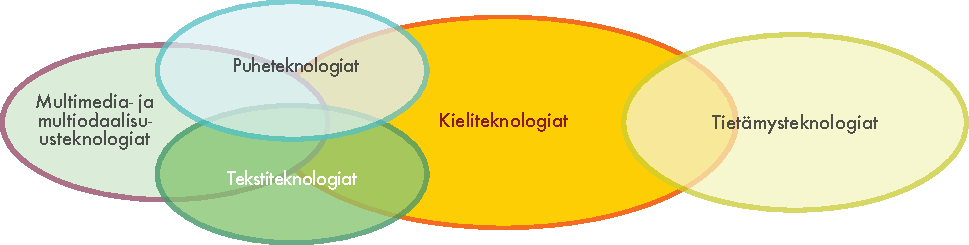
\includegraphics[width=\textwidth]{../_media/finnish/language_technologies}
  \caption{Kieliteknologia kontekstissa}
  \label{fig:ltincontext-fin}
  \colorrule{grey3}{\textwidth}{1.5pt}
\end{figure*}

Seuraavassa tarkastellaan kieliteknologian tärkeimpiä sovellusaloja,
toisin sanoen kielentarkistusta, hakukonetta, puhesovelluksia ja
konekääntämistä.  Sovelluksia ja perusteknologioita ovat mm.
\begin{itemize}
\item oikeinkirjoituksen tarkistus

\item kirjoittajan apuvälineet

\item tietokoneavusteinen kielenoppiminen

\item tiedonhaku

\item tiedon eristäminen

\item lyhennelmän tuottaminen tekstistä

\item kysymysvastausjärjestelmä

\item puheentunnistus ja

\item puhesynteesi.
\end{itemize}

Kieliteknologia on vakiintunut tutkimusala. Peruskirjallisuutta ovat
muun muassa seuraavat viitteet: \cite{carstensen-etal1,
  jurafsky-martin01, manning-schuetze1, lt-world1, lt-survey1}.\\
Ennen sovellusalojen esittelyä kuvataan tyypillisen
kieliteknologiajärjestelmän arkkitehtuuri lyhyesti alla.


\subsection{Sovellusarkkitehtuurit}


Kielenkäsittelyn sovellusohjelmat koostuvat tavallisesti useista
komponenteista, jotka kuvastavat kielen eri ominaisuuksia. Kuva
\ref{fig:textprocessingarch-fin} esittää tyypillisen tekstinkäsittelyn
arkkitehtuurin yksinkertaistetussa muodossa. Ensimmäiset kolme
moduulia kuvaavat tekstinsyötön rakennetta ja tarkoitusta:

\begin{figure*}[b]
  \colorrule{grey3}{\textwidth}{1.5pt}
  \center
  %\vspace{-5mm} 
  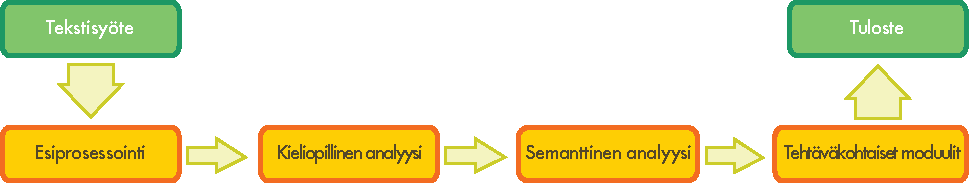
\includegraphics[width=\textwidth]{../_media/finnish/text_processing_app_architecture}
  \caption{Tyypillinen tekstinkäsittelyn arkkitehtuuri}
  \label{fig:textprocessingarch-fin}
  \colorrule{grey3}{\textwidth}{1.5pt}
\end{figure*}

\begin{enumerate}
\item Esiprosessointi puhdistaa dataa, analysoi tai poistaa muotoiluja,
 päättelee lähtökielen, jne.

\item Kieliopillinen analyysi etsii lauseiden verbit, objektit,
määreet ja muut lauseenjäsenet ja päättelee virkerakenteen.

\item Semanttinen analyysi suorittaa yksikäsitteistämisen (laskee
sanojen oikean merkityksen tietyssä käyttöympäristössä), ratkaisee
viittaussuhteet (selvittää mm. virkkeen pronominien viittaukset
substantiiveihin) ja korvaavat ilmaukset, sekä tuottaa virkkeen
merkitysrakenteen koneen luettavassa muodossa.
\end{enumerate}

Tekstin analyysin jälkeen tehtäväkohtaiset moduulit pääsevät
suorittamaan muita operaatioita, kuten automaattista lyhennelmien
tuottamista ja tietokantahakuja.\\
Seuraavassa esitellään ensin kieliteknologian keskeiset sovellusalat.
Sen jälkeen kuvataan lyhyesti kieliteknologian tutkimuksen ja
opetuksen tilanne maassamme sekä tärkeimmät jo päättyneet ja käynnissä
olevat tutkimusohjelmat. Lopuksi kartoitetaan asiantuntijoiden
arvioita keskeisistä kieliteknologian työkaluista ja kieliaineistoista
useiden kriteerien valossa, joita ovat esimerkiksi saatavuus,
valmiusaste ja laatu. Yhteenveto arvioista suomen osalta esitetään
taulukon muodossa (kuva~\ref{fig:lrlttable-fin}). Lisäksi suomen
kielen kieliteknologian tilanne suhteutaan tämän sarjan muihin
kieliin.


\subsection{Keskeiset sovellusalat}


Tässä osiossa keskitytään tärkeimpiin kieliteknologisiin työkaluihin
ja kieliaineistoihin ja luodaan katsaus kieliteknologiaan Suomessa.
Lihavoidut työkalut ja aineistot löytyvät myös
kuvasta~\ref{fig:lrlttable-fin} (s.~\pageref{fig:lrlttable-fin}) luvun
lopussa.



\subsubsection{Kielentarkistus}

Useimmat tekstinkäsittelyohjelmia käyttäneet tietävät, että oikeinkirjoituksen 
tarkistin tuo esiin kirjoitusvirheet niitä korostamalla ja ehdottaa niihin
korjauksia. Ensimmäiset oikeinkirjoitusta tarkistavat ohjelmat
vertasivat tekstistä irrotettuja sanoja sanakirjaan. Tarkistimet ovat niistä ajoista 
kehittyneet, ne tunnistavat jo kielikohtaisten \textbf{kieliopillisen analyysin}
algoritmien avulla sanojen morfologiasta johtuvia virheitä tekstissä 
(esim. monikon muodostus) ja syntaktisia ongelmia, kuten
puuttuvan verbin tai kongruenssivirheen (\textit{me *kirjoittaa
kirjeen}). Useimmat englannin oikeinkirjoituksen tarkistimet eivät kuitenkaan
löydä virheitä seuraavasta englanninkielisestä tekstistä:

\begin{quote}
  I have a spelling checker,\\
  It came with my PC.\\
  It plane lee marks four my revue\\
  Miss steaks aye can knot sea.~\cite{Surprise}
\end{quote}

Tämänkaltaisten virheiden löytyminen edellyttää yleensä tietoa
käyttöympäristöstä, esimerkkinä sen päättäminen, tulisiko sanan alkaa
isolla kirjaimella vai ei:
\begin{itemize}
\item[] \textit{Muista ottaa kaneli mukaan.}

\item[] \textit{Muista ottaa Kaneli mukaan.}
\end{itemize}
Vastaavissa tapauksissa tarvitaan joko
kielikohtaisten \textbf{kielioppien} muotoilemista, toisin
sanoen paljon kielitieteellistä osaamista ja
käsityötä, tai vaihtoehtoisesti voidaan käyttää apuna tilastollisia
kielimalleja laskemaan, millä todennäköisyydellä tietyn sanan voidaan odottaa 
esiintyvän juuri tietyssä ympäristössä sitä edeltävien
tai seuraavien sanojen yhteydessä. \textit{Kaneli} esimerkiksi
esiintyy paljon todennäköisemmin ainesanana kuin
erisnimenä. Tilastollinen kielimalli voidaan johtaa aineistosta
automaattisesti, kunhan käytettävissä on tarpeeksi suuri määrä
(virheetöntä) kieliainesta, eli tehtävään soveltuva
\textbf{tekstikorpus}. Tähän asti tilastollisia malleja on enimmäkseen kehitetty
ja arvioitu englanninkielistä kieliainesta varten. Mallit eivät kuitenkaan
ole siirrettävissä suoraan suomen kielen käsittelyyn, johtuen mm.
suomen suhteellisen vapaasta sanajärjestyksestä, yhdyssanojen
muodostuksesta ja sanojen taipumisesta.

\begin{figure*}[htb]
  \colorrule{grey3}{\textwidth}{1.5pt}
  %\vspace{-9mm}
  \center
  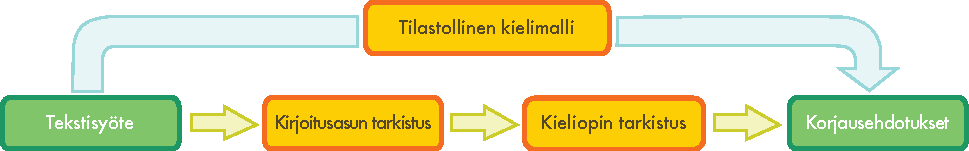
\includegraphics[width=\textwidth]{../_media/finnish/language_checking}
  \caption{Kielentarkistus (tilastollinen; sääntöpohjainen)}
  \label{fig:langcheckingarch-fin}
  \colorrule{grey3}{\textwidth}{1.5pt}
\end{figure*}

Kielentarkistustoiminto ei sisälly ainoastaan
tekstinkäsittelyohjelmiin, vaan se löytyy myös kirjoittajan
apuvälineistä, vaikkapa ohjelmista, joiden avulla kirjoitetaan käsikirjoja ja muuta
dokumentaatiota noudattaen tietyn erikoisalan, esimerkiksi
terveydenhuollon tai rakennustekniikan, usein monimutkaisia
standardeja. Lähdettyään kansainvälisille markkinoille kääntämisen ja 
lokalisoinnin avulla monet yritykset ovat alkaneet
panostaa entistä enemmän teknisen dokumentoinnin laatuun. Ne haluavat
välttyä asiakkaiden valituksilta ja vahingonkorvausvaatimuksilta,
jotka ovat usein tulosta huonosti ymmärretyistä ohjeista johtuvasta
tuotteen virheellisestä käytöstä. Luonnollisen kielen
käsittelyn edistyminen on tuottanut parempia kirjoittajan
apuvälineitä, jotka auttavat teknisen dokumentaation kirjoittajaa 
valitsemaan alan käytänteitä ja yrityksen terminologisia
valintoja noudattavia termejä ja lauserakenteita.
\boxtext{Kielentarkistus on myös kirjoittajan apuväline.}

Suomessa on historiallisista syistä kehittynyt useita pieniä
kieliteknologiayrityksiä ja palveluntarjoajia, joiden tuotteet
perustuvat moniin kielimalleihin. Suomen kieli on haastava kieli
mallinnettavaksi, tai kuten Antti Arppe asian vuonna 2002 ilmaisi:
"Kun esimerkiksi englantia varten pystyy kehittämään yksinkertaisen
kielenkäsittelyohjelmiston kuten oikolukijan käytännössä listaamalla
ja kompressoimalla yleisimmät sata tuhatta sanaa, suomen kohdalla
pitäisi samaa tekniikkaa noudattaen listata jos ei satoja niin
vähintään kymmeniä miljoonia eri sanamuotoja, jotta vastaava
oikolukija olisi yhtä kattava." \cite{EiPolkua} 1980-luvun
loppupuolelta alkaen on seuraavilla kieliteknologiayrityksillä ollut
tuotevalikoimissaan kielentarkistusohjelmia: nykyisin sanakirjoihin erikoistunut
Kielikone, kielen analyysin työkaluija tarjoava Connexor, itseorganisoituvia 
karttoja (SOM) hyödyntävä Gurusoft ja Lingsoft, joka tarjoaa laajan valikoiman 
tuotteita suomen kielelle.\\
Kielentarkistus on tärkeää oikeinkirjoituksen tarkistinten ja
kirjoittajan apuvälineiden lisäksi tietokoneavusteisessa
kielenoppimisessa.  Kielentarkistuksen sovellukset voivat myös
automaattisesti korjata hakukoneiden hakulausekkeita, jolloin
esimerkiksi Google ehdottaa sopivia hakutuloksia myös sellaisten
sanojen perusteella, joissa on jokin kirjoitusvirhe.



\subsubsection{Hakukoneet}


Tiedon hakeminen verkosta, suljetusta intranetistä tai sähköisistä
kirjastoista on todennäköisesti eniten käytetty, mutta
vielä kehitysasteella oleva kieliteknologinen sovellus. Googlen
hakukone, joka aloitti toimintansa vuonna 1998 käsittelee tänään noin
80\% kaikista hakukyselyistä \cite{spi1}. Suomen puhekieleen on
ilmestynyt uusi verbi \textit{guuglata}, jolle ei vielä
ole vakiintunutta kirjoitusasua. Google korjaa nykyisin kirjoitusvirheen
sisältävän hakusanan kirjoitusasun automaattisesti, ja kyselyissä hyödynnetään
merkityksen analysointia. Osumatarkkuus paranee, kun termien 
merkitys määritellään niiden käyttöympäristön perusteella \cite{Google-rolls}. 
Googlen menestystarina osoittaa, että kun käytettävissä on suuria määriä 
materiaalia ja tehokkaat indeksointitekniikat, tuottaa tilastolliseen malliin
perustuva menetelmä tyydyttäviä tuloksia.\\
Kehittyneempiä tiedonhakutarpeita varten on syytä yhdistää
syvempi kielitieteellinen tietämys \textbf{semanttiseen analyysiin}.
Kokeilut, joissa on hyödynnetty \textbf{leksikaalisia resursseja} kuten koneluettavat
käsitesanakirjat tai ontologiapohjaiset kieliresurssit
(esim. FinnWordNet) ovat osoittaneet edistymistä osumatarkkuudessa, kun niiden 
avulla on voitu hyödyntää alkuperäisten hakusanojen ja termien synonyymejä, kuten
\textit{atomienergia},
\textit{atomivoima} ja
\textit{ydinenergia}
ja myös vähemmän toisiinsa sidoksissa olevia termejä
voidaan hyödyntää.

\begin{figure*}[htb]
  \colorrule{grey3}{\textwidth}{1.5pt}
  %\vspace{-9mm}
  \center
  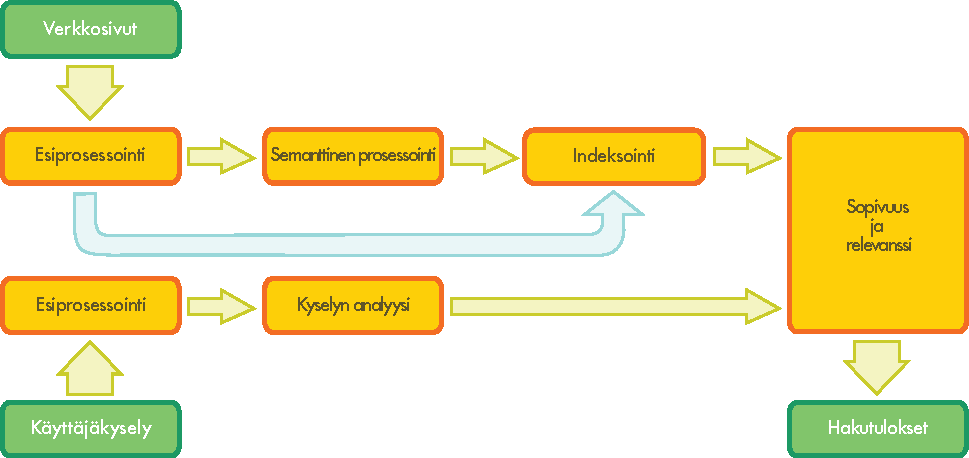
\includegraphics[width=\textwidth]{../_media/finnish/web_search_architecture}
  \caption{Haku verkossa}
  \label{fig:websearcharch-fin}
  \colorrule{grey3}{\textwidth}{1.5pt}
 \end{figure*}

\boxtext{Tulevaisuuden hakukoneet perustuvat kehittyneempään kieliteknologiaan.}

Seuraavan hakukoneiden sukupolven on syytä perustua paljon
kehittyneempään kieliteknologiaan, kun tavoitteena on
pystyä vastaamaan myös hakukyselyyn, joka muodostuu
avainsanojen sijaan kysymyksestä. Löytääkseen vastauksen kyselyyn “Anna lista 
kaikista yrityksistä, jotka jokin toinen yritys on ostanut viimeisen viiden vuoden aikana”,
kieliteknologisen järjestelmän tulee analysoida virkkeen rakenne ja merkitys 
sekä tuottaa indeksi oikeiden dokumenttien löytämiseksi riittävän nopeasti. 
Hyvän hakutuloksen tuottaminen edellyttää virkkeen kieliopillisen rakenteen
analysointia, jotta järjestelmä osaa päätellä, että hakija tarvitsee
tietoa ostetuista eikä muita ostaneista yrityksistä. Ilmaisun
\textit{viimeisen viiden vuoden} tulkintaa varten järjestelmän tulee
pystyä päättelemään, mitkä vuodet ovat kyselyn ajankohtaan nähden
relevantteja. Ja lopulta on verrattava hakukyselyä valtavaan määrään
rakenteistamatonta tietoainesta, jotta löytyy juuri hakijan tarvitsema palanen 
tietoa. Tiedonhakuprosessi sisältää siten relevanttien dokumenttien löytämisen ja 
järjestämisen paremmuusjärjestykseen. Tuottaakseen listauksen yrityksistä 
järjestelmän täytyy myös tunnistaa tietty merkkijono tai sana\-jono dokumentissa yrityksen
nimeksi. Tätä kutsutaan nimellä “named entity
recognition”.\\
Vaativampi haaste on tietynkielisen kyselyn yhdistäminen muunkielisiin
dokumentteihin. Kieltenvälinen tiedonhaku sisältää kyselyn
automaattisen kääntämisen kaikille mahdollisille lähtökielille ja sen
jälkeen tulosten kääntämisen takaisin kohdekielelle.\\
Tietoa varastoidaan nykyisin entistä enemmän muutoinkin kuin
tekstinä. Tarvitaan multimediatiedonhakua, kun etsitään kuvia, 
äänitiedostoja ja videomateriaalia. Ääni- ja videotiedostojen käsittelyssä 
puheentunnistuksen moduulin tulee muuntaa puheaines tekstiksi 
(tai foneettiseen muotoon), jotta sitä voidaan verrata käyttäjän kyselyyn.\\
Suomessa on vain muutama aktiivisesti hakuteknologioita kehittävä ja soveltava 
pienyritys. Gurusoft on erikoistunut kielestä riippumattomiin itseorganisoituviin 
karttoihin (SOM) ja soveltaa niihin perustuvia menetelmiä tiedonhaun tehtäviin, 
mutta yrityksen Docunaut-tuote on kehitetty asiakkaiden sisäisten intranettien kyselyihin
maailmanlaajuisen Internetin sijaan. Raportin kirjoittamisen aikaan ei
Suomessa ole vireillä laajamittaisia hakukoneteknologiaprojekteja.



\subsubsection{Puheteknologia}

Puheeseen perustuva vuorovaikutus kuuluu sovellusaloihin, jotka
tarvitsevat puheteknologiaa eli teknologioita, joilla käsitellään
puhuttua kieltä. Puheeseen pohjautuva koneen käyttö ei tapahdu
graafisella näytöllä, näppäimistöllä tai hiirellä vaan puhutulla
kielellä.
\boxtext{Puheteknologioita tarvitaan, kun halutaan kommunikoida koneen kanssa puheen avulla.}
Puhekäyttöliittymiä (Voice User Interface, VUI) käytetäänkin nykyään usein osittain tai täysin
automatisoiduissa puhelinpalveluissa. Erityisen paljon niitä hyödyntäviä aloja ovat 
rahoitus, hankinta-ala, julkinen liikenne ja tietoliikenne. Muita
puhekäyttöliittymien sovelluskohteita ovat mm. ajoneuvojen
navigointilaitteistot ja puhe graafisen näytön tai kosketusnäytön
vaihtoehtona älypuhelimen ohjaamisessa.

Puhepohjaiseen vuorovaikutukseen kuuluu neljä aluetta:

\begin{enumerate}
\item Automaattinen \textbf{puheentunnistus} määrittelee, mitkä sanat
  todella sisältyvät tiettyyn äänten sekvenssiin käyttäjän tuottamassa
  puheessa.
\item Luonnollisen kielen ymmärtäminen käsittää puheeseen sisältyvän
  ilmaisun syntaktisen rakenteen analyysin ja sen tulkinnan kyseisen
  järjestelmän mukaisesti.
\item Dialoginhallinta päättelee, mihin toimenpiteisiin on syytä
  ryhtyä ottaen huomioon käyttäjän antama syöte ja järjestelmän
  toimintaperiaate.
\item \textbf{Puhesynteesi} muuttaa järjestelmän vastauksen ääneksi
  käyttäjää varten.
\end{enumerate}

\begin{figure*}[htb]
  \colorrule{grey3}{\textwidth}{1.5pt}
  %\vspace{-9mm}
  \center  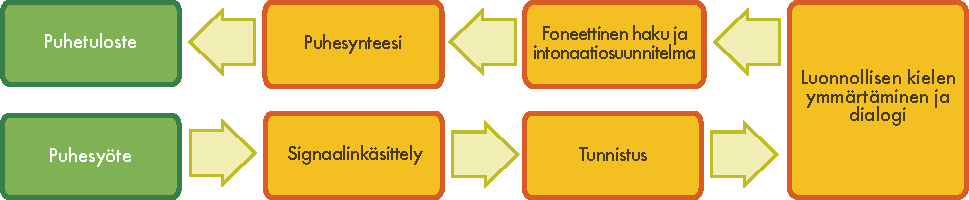
\includegraphics[width=\textwidth]{../_media/finnish/simple_speech-based_dialogue_architecture}
  \center
    \caption{Puheeseen pohjautuva dialogijärjestelmä}
    \label{fig:dialoguearch-fin}
    \colorrule{grey3}{\textwidth}{1.5pt}
  \end{figure*}

Eräs puheteknologiajärjestelmien haasteista on tunnistaa käyttäjän
puheesta sanat oikein. Tämä merkitsee käytännössä käyttäjän
puheilmausten rajoittamista siten, että mahdollinen syöte saa sisältää vain rajoitetun
asiasanalistan jäseniä. Toinen vaihtoehto on luoda käsityönä kielimalleja,
jotka kattavat suuren määrän luonnollisen kielenkäytön kokonaisia
ilmauksia. Koneoppimisen teknologioiden avulla voidaan kielimallit
myös tuottaa automaattisesti laajoista \textbf{puhekorpuksista}, jotka ovat
puhutun kielen kokoelmia puheäänitiedostoineen ja tekstin
transkriptioineen. Ilmausten rajoittaminen pakottaa kuitenkin ihmiset
käyttämään puhekäyttöliittymää ennalta määritellyllä tavalla, mikä heikentää järjestelmän
käytettävyyttä. Toisaalta kattavien kielimallien luominen, hienosäätö
ja ylläpito nostavat kustannuksia. Puhekäyttöliittymät, jotka hyödyntävät kielimalleja ja
heti alussa antavat käyttäjän kertoa asiansa joustavammin —
ja aloittavat vaikkapa tervehtimällä asiakasta ilmauksella \textit{Miten voin auttaa?} — ovat usein
pitkälle automatisoituja ja siten käyttäjien helpommin hyväksyttävissä ihmisen korvaajaksi.\\
Yritykset tapaavat käyttää ammattipuhujien etukäteen äänittämää
puhemateriaalia suoraan puhekäyttöliittymän tuottamiksi ilmauksiksi. Kun
ilmaus on pysyvää laatua, eikä sen sanamuoto riipu käyttöympäristöstä tai
käyttäjäkohtaisesta tiedosta, voi menetelmä tuottaa miellyttävän
käyttäjäkokemuksen. Mutta tulos voi tuntua epäluonnolliselta, 
koska äänitiedostojen palaset on menetelmässä yksinkertaisesti liimattu yhteen. 
Uuden teknologian puhesynteesijärjestelmät ovat tässä suhteessa edeltäjiään parempia, 
kun luonnollisuus on otettu selkeämmin tavoitteeksi.\\
Puheteknologiasovellusten käyttöliittymien teknologiset komponentit
ovat olleet laajan standardointityön kohteena kuluneen vuosikymmenen
aikana. Puheentunnistuksen ja puhesynteesin markkinat ovat samalla keskittyneet. 
Viisi alan globaalia toimijaa ovat hallinneet G20-valtioiden 
(taloudellisesti kestävällä pohjalla olevien valtioiden) kansallisia markkinoita, 
joista yhdysvaltalainen Nuance ja italialainen Loquendo ovat olleet vahvoja Euroopan
markkinoilla. Vuonna 2011 Nuance ilmoitti ostaneensa Loquendon, mikä
osoittaa markkinoiden keskittyvän edelleen.\\
Puheteknologian tutkimusta on tehty Suomessa 1960-luvulta asti ja
tuloksena on ollut kansainvälisestikin vaikuttavia tuotteita,
esimerkiksi kannettava Synte 2 -puhesynteesi, joka kehitettiin
silloisen Teknillisen korkeakoulun (nykyinen Aalto-yliopisto)
akustiikan ja äänenkäsittelytekniikan laboratoriossa 1970-luvulla. Toinen esimerkki on 
1980-luvulla kehitetty foneettinen kirjoituskone. Joitakin yksittäisiä
puheteknologisia tuotteita on myös tuotu markkinoille 1990-luvun alun
jälkeen, mutta niiden asiakaskunta on rajoittunut lähinnä
erityisryhmiin. Sekä julkisella että yksityisellä sektorilla on panostettu 
merkittäviin tutkimus- ja kehityshankkeisiin, jotka alkavat tuottaa tulosta 
– niiden ansiosta on suomen kielelle
nyt tarjolla useita sekä puheentunnistuksen että puhesynteesin
teknologioita hyödyntäviä tuotteita, jotka yltävät samalle tasolle
muille kielille tehtyjen tuotteiden kanssa. Useimmat suomalaiset
kansainvälisellä tasolla toimivat puheteknologiayritykset tarjoavat
suomen kielelle sekä puhesynteesiä että automaattista
puheentunnistusta. Kaksi suomalaista yritystä, Bitlips Oy ja Timehouse
Oy, tarjoavat suomenkielistä puhesynteesiä. Lingsoft Oy sekä Suomen
Puheentunnistus Oy ovat molemmat tuotteistaneet suomen kielen
automaattisen puheentunnistuksen järjestelmiä ja ne tuottavat
puhekäyttöliittymiä useille suomalaisille yrityksille.\\
Suomessa on käynnissä useita mittavia tutkimushankkeita sekä
puhesynteesin että automaattisen puheentunnistuksen puolella. Pääosa
tutkimuksesta tehdään Aalto-yliopistossa, Helsingin yliopistossa ja
Tampereen teknillisessä korkeakoulussa. Isoin teollinen toimija
puheentutkimuksen alueella Suomessa on perinteisesti ollut Nokia.\\
Dialoginhallintaan liittyvän teknologian ja osaamisen saralla ei
Suomessa ole pienyrityksiä, jotka tarjoaisivat alan tuotteita. Puheen
vuorovaikutustekniikoiden alalla ei vielä ole aitoa markkinatilannetta.\\
Tulevaisuudessa on odotettavissa merkittäviä muutoksia älypuhelinten
yleistyessä. Ne tarjoavat uuden alustan asiakassuhteiden
ylläpitoon perinteisten viestimien, Internetin ja sähköpostin
lisäksi, myös vuorovaikutteisten sovellusten kysyntä kasvaa. Pitkällä tähtäimellä
puhelimeen sisältyviä puhekäyttöliittymiä tulee olemaan tarjolla
vähemmän ja puheen rooli käyttäjäystävällisenä älypuhelimen
komentokielenä tulee olemaan entistä paljon keskeisemmässä
roolissa. Kehitystä tulee erityisesti vauhdittamaan puhujasta
riippumattomien puheentunnistusmenetelmien tarkkuuden asteittainen
paraneminen.  Sanelujärjestelmiä on jo tarjolla älypuhelinten
käyttäjille keskitettyinä palveluina.


\subsubsection{Konekääntäminen}

Idea tietokoneiden hyödyntämisestä luonnollisten kielten
kääntämisessä syntyi jo vuonna 1946, ja ala sai merkittävää 
tutkimusrahoitusta heti 1950-luvulla ja uudelleen 1980-luvulla. Siitä
huolimatta ei \textbf{konekääntämisen} (MT) alalla vielä tähän päivään mennessä
ole pystytty saavuttamaan alkuperäistä tavoitetta kaikkien
käytettävissä olevasta automaattisesta kääntimestä.\\
Konekääntämisen peruslähtökohta on korvata yhdellä luonnollisella
kielellä kirjoitetun tekstin sanat automaattisesti toisen kielen
vastineilla.  Lähestymistapa voi olla hyödyllinen
tapauksessa, jossa tekstit käsittelevät sellaisia aihealueita, joiden
kieli on hyvin rajoittunutta ja muodollista, kuten esimerkiksi
sääraportteja. Mutta kun tavoitteena on tuottaa laadukas käännös
vähemmän standardoidusta aineksesta, on siirryttävä yhdistämään
isompia tekstin yksiköitä niiden lähimpiin kohdekielen
vastineisiin. Suurin ongelma syntyy luonnollisen kielen
monimerkityksisyydestä. Se on haasteellista monella tasolla, kuten
sanaston yksiköiden merkitysten disambiguointi eli
yksikäsitteistäminen (jaguaari on sekä automerkki että kissaeläin) tai
taivutuspäätteen tulkinta syntaksin tasolla, esimerkiksi:

\begin{itemize}
\item[] \textit{Poliisi tarkkaili miestä mäellä.}

\item[] \textit{Poliisi tarkkaili miestä kiikarilla.}
\end{itemize}

Konekäännösjärjestelmiä voidaan rakentaa myös hyödyntämällä
kielitieteellisiä sääntöjä. Kun kääntäminen tapahtuu sukukielten
välillä, voi suoran korvaamisen menetelmä olla järkevä. Mutta sääntöpohjaiset (tai
kielitieteelliseen tietoon pohjautuvat) järjestelmät usein analysoivat
lähtötekstin ja luovat symbolisen representaation välivaiheen, josta
kohdekielinen teksti voidaan sitten generoida. Näiden menetelmien
toimivuus ja lopputuloksen laatu ovat täysin riippuvaisia siitä, onko saatavilla laajoja
sanastoja, joihin morfologista, syntaktista ja semanttista tietoa on
koodattu ja onko asiansa osaavien lingvistien koostamia laajoja
kieliopillisten sääntöjen kokoelmia käytettävissä. Kokonaisuudessaan prosessi on
pitkä ja tulee siksi usein kalliiksi.
\boxtext{Konekääntämisessä korvataan lähtökielen sanat automaattisesti kohdekielen sanoilla.}

1980-luvun loppupuolella, kun tietokoneiden tehokkuus kasvoi ja
tekniikka halpeni, kiinnostus konekääntämisen tilastollisia malleja
kohtaan heräsi jälleen. Tilastolliset mallit ovat kehittyneet
kaksikielisten tekstikorpusten analysoinnin pohjalta, esimerkkinä
Europarl-\textbf{rinnakkaiskorpus}, joka sisältää Euroopan parlamentin
puheenvuorot 21 eurooppalaisella kielellä. Kun aineistoa on tarpeeksi,
tilastollinen konekäännin saavuttaa riittävän tarkkuuden tuottamalla
vieraan kielen merkityksen likiarvoja. Se tuottaa todennäköisistä
sanoista muodostuvia jatkumoita tekstien rinnakkaisista
versioista. Mutta toisin kuin tietämykseen perustuvat järjestelmät,
tilastolliset (tai aineistopohjaiset) konekääntimet tuottavat usein
kieliopillisesti heikkoa tulosta.  Aineistopohjaisen konekääntämisen
hyöty syntyy siitä, että se edellyttää vähemmän inhimillistä työtä ja
kattaa myös kielikohtaisia ominaispiirteitä (esim. idiomaattiset
ilmaukset), jotka saattava jäädä ilman huomiota tietämyspohjaisissa
järjestelmissä.

\begin{figure*}[htb]
  \colorrule{grey3}{\textwidth}{1.5pt}
  %\vspace{-21mm}
  \center
  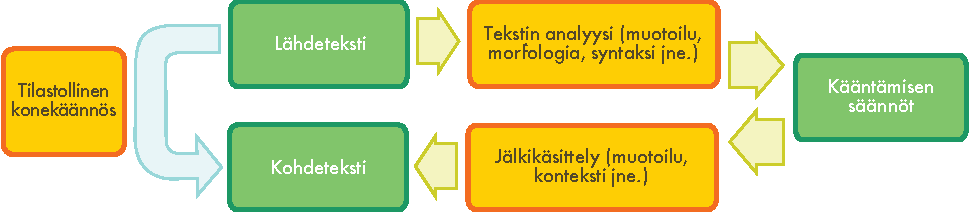
\includegraphics[width=\textwidth]{../_media/finnish/machine_translation}
  \caption{Konekäännös (tilastollinen; sääntöpohjainen)}
  \label{fig:mtarch-fin}
  \colorrule{grey3}{\textwidth}{1.5pt}
\end{figure*}

Tietämyspohjaisen ja aineistopohjaisen konekääntämisen vahvuudet ja
heikkoudet tapaavat olla toisiaan täydentäviä, joten nykyisin tutkijat
keskittyvät molemmat menetelmät yhdistäviin hybridiratkaisuihin. 
On myös kokeiltu lähestymistapaa, jossa käytetään sekä tietämyspohjaisia että
aineistopohjaisia järjestelmiä yhdessä, jolloin tarvitaan erillinen valintaosio 
tekemään valinta vaihtoehtoisisten vastineiden välillä.  Tulokset pidempien kuin noin 12 sanan 
virkkeiden osalta ovat usein vähemmän hyviä. Paremmaksi ratkaisuksi on osoittautunut 
parhaiden palojen yhdistäminen useammasta vastineeksi ehdotetusta virkkestä. 
Tällöin prosessi voi tosin olla suhteellisen monimutkainen, kun
ei aina ole ilmeistä, mitkä palaset monista vaihtoehdoista parhaiten vastaavat
toisiaan, ja palaset tulisi lisäksi pystyä kohdistamaan toisiinsa
luotettavasti.
\boxtext{Konekääntäminen on erityisen haastavaa suomen kielen osalta.}

Suomi ei ehtinyt mukaan ensimmäisen sukupolven konekäännöshankkeisiin,
mutta tuli mukaan toisessa aallossa sääntöpohjaisen konekääntimen
kehittämiseen 1980-luvulla. Pitkän tähtäimen kansallisesti rahoitettu
tutkimus- ja kehityshanke Kielikone kehitti ensin tarpeelliset suomen
kielen analyysityökalut ja käytti sitten niitä rakentaakseen
sääntöpohjaisen suomi-englanti konekäännössovelluksen 1990-luvulla,
josta sittemmin syntyi kaupallinen tuote. IBM Finland tutki omaan
englannin jäsentimeensä perustuvaa englanti-suomi suuntaa 90-luvun
vaihteessa, mutta projekti ei päässyt tuotantoon asti. Nykyisin Sunda,
joka käyttää Kielikoneen teknologian pohjalta kehitettyä uudempaa
sääntöpohjaista järjestelmää, myy suhteellisen hyvälaatuista
englanti-suomi konekäännöstuotetta. Google ja Microsoft tarjoavat
suomen tilastollista konekäännöstä, mutta laatu jää heikoksi johtuen
suomen morfologian kompleksisuudesta sekä suhteellisen vapaasta
sanajärjestyksestä, joka kuten yllä on todettu, on haaste nykyisille
tilastollisille konekäännösjärjestelmille. Aalto-yliopistossa toimiva
tutkimusryhmä työskentelee suomen kielen morfologian ja tilastollisen
konekäännöksen kysymysten parissa.\\
Konekäännösjärjestelmien laadun parantamisessa on jatkossa paljon
potentiaalia. Haasteena ovat kieliresurssien sovittaminen tietyn alan
tarpeisiin ja toisaalta teknologian integrointi työnkulun prosesseihin, joihin 
termitietokannat ja käännösmuistit jo sisältyvät. Lisäksi useimmat nykyisistä 
järjestelmistä ovat on tehty englannin kääntämistä varten, ja tukea
löytyy vain harvalle kielelle suomesta tai suomeen käännettäessä. Käännöksen 
työnkulku monimutkaistuu, jos konekäännöohjelman käyttäjä joutuu opettelemaan 
erilaisia sanaston koodaustyökaluja eri järjestelmiä varten.\\
Konekäännösjärjestelmien arviointihankkeiden tulokset auttavat niiden
laadun vertailussa, ne selventävät eri lähestymistapoja ja tarjoavat
tietoa siitä, millaisessa tilanteessa eri kieliparit ovat. Kuva
\ref{fig:euromatrix} sisältää Euromatrix+ -projektin aikana kootut
tuolloin 22 virallisen EU-kielen tulokset kielipareittain (iiri ei
ollut vertailussa mukana). Tulokset on arvioitu BLEU-pistein, joissa
paremman käännöksen pistemäärä on aina korkeampi \cite{BLEU}. Ihminen
saisi käännöstehtävästä keskimäärin 80 pistettä.\\
Parhaimmat pisteet (taulukossa vihreällä ja sinisellä värillä) saivat
kielet, joihin on panostettu perustamalla yhteistyöprojekteja ja
joiden tutkijoilla on käytössään useita rinnakkaiskorpuksia
(esimerkkeinä englanti, ranska, hollanti, espanja ja
saksa). Taulukossa on punaisella merkitty huonoimmat tulokset.  Näiden
kielten kehittämiseen ei joko ole panostettu hankerahoitusta tai ne
ovat rakenteellisesti erityisen paljon muista tutkituista kielistä
poikkeavia (esimerkkeinä unkari, malta ja suomi).

\begin{figure*}[tb]
  \centering
  \setlength{\tabcolsep}{0.17em}
  \small
  \begin{tabular}{>{\columncolor{corange1}}cccccccccccccccccccccccc}
  & \multicolumn{22}{>{\columncolor{corange1}}c}{Kohdekieli -- Target Language}\\\addlinespace[{-.009cm}]
  \rowcolor{corange1}  & EN & BG & DE & CS & DA & EL & ES & ET & FI & FR & HU & IT & LT & LV & MT & NL & PL & PT & RO & SK & SL & SV\\
  EN & -- & \textcolor{blue}{40.5} & \textcolor{blue}{46.8} & \textcolor{green2}{52.6} & \textcolor{green2}{50.0} & \textcolor{blue}{41.0} & \textcolor{green2}{55.2} & \textcolor{purple}{34.8} & \textcolor{purple}{38.6} & \textcolor{green2}{50.1} & \textcolor{purple}{37.2} & \textcolor{green2}{50.4} & \textcolor{purple}{39.6} & \textcolor{blue}{43.4} & \textcolor{purple}{39.8} & \textcolor{green2}{52.3} & \textcolor{blue}{49.2} & \textcolor{green2}{55.0} & \textcolor{blue}{49.0} & \textcolor{blue}{44.7} & \textcolor{green2}{50.7} & \textcolor{green2}{52.0}\\
  BG & \textcolor{green}{61.3} & -- & \textcolor{purple}{38.7} & \textcolor{purple}{39.4} & \textcolor{purple}{39.6} & \textcolor{purple}{34.5} & \textcolor{blue}{46.9} & \textcolor{red3}{25.5} & \textcolor{red3}{26.7} & \textcolor{blue}{42.4} & \textcolor{red3}{22.0} & \textcolor{blue}{43.5} & \textcolor{red3}{29.3} & \textcolor{red3}{29.1} & \textcolor{red3}{25.9} & \textcolor{blue}{44.9} & \textcolor{purple}{35.1} & \textcolor{blue}{45.9} & \textcolor{purple}{36.8} & \textcolor{purple}{34.1} & \textcolor{purple}{34.1} & \textcolor{purple}{39.9}\\
  DE & \textcolor{green2}{53.6} & \textcolor{red3}{26.3} & -- & \textcolor{purple}{35.4} & \textcolor{blue}{43.1} & \textcolor{purple}{32.8} & \textcolor{blue}{47.1} & \textcolor{red3}{26.7} & \textcolor{red3}{29.5} & \textcolor{purple}{39.4} & \textcolor{red3}{27.6} & \textcolor{blue}{42.7} & \textcolor{red3}{27.6} & \textcolor{purple}{30.3} & \textcolor{red2}{19.8} & \textcolor{green2}{50.2} & \textcolor{purple}{30.2} & \textcolor{blue}{44.1} & \textcolor{purple}{30.7} & \textcolor{red3}{29.4} & \textcolor{purple}{31.4} & \textcolor{blue}{41.2}\\
  CS & \textcolor{green2}{58.4} & \textcolor{purple}{32.0} & \textcolor{blue}{42.6} & -- & \textcolor{blue}{43.6} & \textcolor{purple}{34.6} & \textcolor{blue}{48.9} & \textcolor{purple}{30.7} & \textcolor{purple}{30.5} & \textcolor{blue}{41.6} & \textcolor{red3}{27.4} & \textcolor{blue}{44.3} & \textcolor{purple}{34.5} & \textcolor{purple}{35.8} & \textcolor{red3}{26.3} & \textcolor{blue}{46.5} & \textcolor{purple}{39.2} & \textcolor{blue}{45.7} & \textcolor{purple}{36.5} & \textcolor{blue}{43.6} & \textcolor{blue}{41.3} & \textcolor{blue}{42.9}\\
  DA & \textcolor{green2}{57.6} & \textcolor{red3}{28.7} & \textcolor{blue}{44.1} & \textcolor{purple}{35.7} & -- & \textcolor{purple}{34.3} & \textcolor{blue}{47.5} & \textcolor{red3}{27.8} & \textcolor{purple}{31.6} & \textcolor{blue}{41.3} & \textcolor{red3}{24.2} & \textcolor{blue}{43.8} & \textcolor{red3}{29.7} & \textcolor{purple}{32.9} & \textcolor{red3}{21.1} & \textcolor{blue}{48.5} & \textcolor{purple}{34.3} & \textcolor{blue}{45.4} & \textcolor{purple}{33.9} & \textcolor{purple}{33.0} & \textcolor{purple}{36.2} & \textcolor{blue}{47.2}\\
  EL & \textcolor{green2}{59.5} & \textcolor{purple}{32.4} & \textcolor{blue}{43.1} & \textcolor{purple}{37.7} & \textcolor{blue}{44.5} & -- & \textcolor{green2}{54.0} & \textcolor{red3}{26.5} & \textcolor{red3}{29.0} & \textcolor{blue}{48.3} & \textcolor{red3}{23.7} & \textcolor{blue}{49.6} & \textcolor{red3}{29.0} & \textcolor{purple}{32.6} & \textcolor{red3}{23.8} & \textcolor{blue}{48.9} & \textcolor{purple}{34.2} & \textcolor{green2}{52.5} & \textcolor{purple}{37.2} & \textcolor{purple}{33.1} & \textcolor{purple}{36.3} & \textcolor{blue}{43.3}\\
  ES & \textcolor{green}{60.0} & \textcolor{purple}{31.1} & \textcolor{blue}{42.7} & \textcolor{purple}{37.5} & \textcolor{blue}{44.4} & \textcolor{purple}{39.4} & -- & \textcolor{red3}{25.4} & \textcolor{red3}{28.5} & \textcolor{green2}{51.3} & \textcolor{red3}{24.0} & \textcolor{green2}{51.7} & \textcolor{red3}{26.8} & \textcolor{purple}{30.5} & \textcolor{red3}{24.6} & \textcolor{blue}{48.8} & \textcolor{purple}{33.9} & \textcolor{green2}{57.3} & \textcolor{purple}{38.1} & \textcolor{purple}{31.7} & \textcolor{purple}{33.9} & \textcolor{blue}{43.7}\\
  ET & \textcolor{green2}{52.0} & \textcolor{red3}{24.6} & \textcolor{purple}{37.3} & \textcolor{purple}{35.2} & \textcolor{purple}{37.8} & \textcolor{red3}{28.2} & \textcolor{blue}{40.4} & -- & \textcolor{purple}{37.7} & \textcolor{purple}{33.4} & \textcolor{purple}{30.9} & \textcolor{purple}{37.0} & \textcolor{purple}{35.0} & \textcolor{purple}{36.9} & \textcolor{red3}{20.5} & \textcolor{blue}{41.3} & \textcolor{purple}{32.0} & \textcolor{purple}{37.8} & \textcolor{red3}{28.0} & \textcolor{purple}{30.6} & \textcolor{purple}{32.9} & \textcolor{purple}{37.3}\\
  FI & \textcolor{blue}{49.3} & \textcolor{red3}{23.2} & \textcolor{purple}{36.0} & \textcolor{purple}{32.0} & \textcolor{purple}{37.9} & \textcolor{red3}{27.2} & \textcolor{purple}{39.7} & \textcolor{purple}{34.9} & -- & \textcolor{red3}{29.5} & \textcolor{red3}{27.2} & \textcolor{purple}{36.6} & \textcolor{purple}{30.5} & \textcolor{purple}{32.5} & \textcolor{red2}{19.4} & \textcolor{blue}{40.6} & \textcolor{red3}{28.8} & \textcolor{purple}{37.5} & \textcolor{red3}{26.5} & \textcolor{red3}{27.3} & \textcolor{red3}{28.2} & \textcolor{purple}{37.6}\\
  FR & \textcolor{green}{64.0} & \textcolor{purple}{34.5} & \textcolor{blue}{45.1} & \textcolor{purple}{39.5} & \textcolor{blue}{47.4} & \textcolor{blue}{42.8} & \textcolor{green}{60.9} & \textcolor{red3}{26.7} & \textcolor{purple}{30.0} & -- & \textcolor{red3}{25.5} & \textcolor{green2}{56.1} & \textcolor{red3}{28.3} & \textcolor{purple}{31.9} & \textcolor{red3}{25.3} & \textcolor{green2}{51.6} & \textcolor{purple}{35.7} & \textcolor{green}{61.0} & \textcolor{blue}{43.8} & \textcolor{purple}{33.1} & \textcolor{purple}{35.6} & \textcolor{blue}{45.8}\\
  HU & \textcolor{blue}{48.0} & \textcolor{red3}{24.7} & \textcolor{purple}{34.3} & \textcolor{purple}{30.0} & \textcolor{purple}{33.0} & \textcolor{red3}{25.5} & \textcolor{purple}{34.1} & \textcolor{red3}{29.6} & \textcolor{red3}{29.4} & \textcolor{purple}{30.7} & -- & \textcolor{purple}{33.5} & \textcolor{red3}{29.6} & \textcolor{purple}{31.9} & \textcolor{red2}{18.1} & \textcolor{purple}{36.1} & \textcolor{red3}{29.8} & \textcolor{purple}{34.2} & \textcolor{red3}{25.7} & \textcolor{red3}{25.6} & \textcolor{red3}{28.2} & \textcolor{purple}{30.5}\\
  IT & \textcolor{green}{61.0} & \textcolor{purple}{32.1} & \textcolor{blue}{44.3} & \textcolor{purple}{38.9} & \textcolor{blue}{45.8} & \textcolor{blue}{40.6} & \textcolor{red3}{26.9} & \textcolor{red3}{25.0} & \textcolor{red3}{29.7} & \textcolor{green2}{52.7} & \textcolor{red3}{24.2} & -- & \textcolor{red3}{29.4} & \textcolor{purple}{32.6} & \textcolor{red3}{24.6} & \textcolor{green2}{50.5} & \textcolor{purple}{35.2} & \textcolor{green2}{56.5} & \textcolor{purple}{39.3} & \textcolor{purple}{32.5} & \textcolor{purple}{34.7} & \textcolor{blue}{44.3}\\
  LT & \textcolor{green2}{51.8} & \textcolor{red3}{27.6} & \textcolor{purple}{33.9} & \textcolor{purple}{37.0} & \textcolor{purple}{36.8} & \textcolor{red3}{26.5} & \textcolor{red3}{21.1} & \textcolor{purple}{34.2} & \textcolor{purple}{32.0} & \textcolor{purple}{34.4} & \textcolor{red3}{28.5} & \textcolor{purple}{36.8} & -- & \textcolor{blue}{40.1} & \textcolor{red3}{22.2} & \textcolor{purple}{38.1} & \textcolor{purple}{31.6} & \textcolor{purple}{31.6} & \textcolor{red3}{29.3} & \textcolor{purple}{31.8} & \textcolor{purple}{35.3} & \textcolor{purple}{35.3}\\
  LV & \textcolor{green2}{54.0} & \textcolor{red3}{29.1} & \textcolor{purple}{35.0} & \textcolor{purple}{37.8} & \textcolor{purple}{38.5} & \textcolor{red3}{29.7} & \textcolor{red2}{8.0} & \textcolor{purple}{34.2} & \textcolor{purple}{32.4} & \textcolor{purple}{35.6} & \textcolor{red3}{29.3} & \textcolor{purple}{38.9} & \textcolor{purple}{38.4} & -- & \textcolor{red3}{23.3} & \textcolor{blue}{41.5} & \textcolor{purple}{34.4} & \textcolor{purple}{39.6} & \textcolor{purple}{31.0} & \textcolor{purple}{33.3} & \textcolor{purple}{37.1} & \textcolor{purple}{38.0}\\
  MT & \textcolor{green}{72.1} & \textcolor{purple}{32.2} & \textcolor{purple}{37.2} & \textcolor{purple}{37.9} & \textcolor{purple}{38.9} & \textcolor{purple}{33.7} & \textcolor{blue}{48.7} & \textcolor{red3}{26.9} & \textcolor{red3}{25.8} & \textcolor{blue}{42.4} & \textcolor{red3}{22.4} & \textcolor{blue}{43.7} & \textcolor{purple}{30.2} & \textcolor{purple}{33.2} & -- & \textcolor{blue}{44.0} & \textcolor{purple}{37.1} & \textcolor{blue}{45.9} & \textcolor{purple}{38.9} & \textcolor{purple}{35.8} & \textcolor{blue}{40.0} & \textcolor{blue}{41.6}\\
  NL & \textcolor{green2}{56.9} & \textcolor{red3}{29.3} & \textcolor{blue}{46.9} & \textcolor{purple}{37.0} & \textcolor{blue}{45.4} & \textcolor{purple}{35.3} & \textcolor{blue}{49.7} & \textcolor{red3}{27.5} & \textcolor{red3}{29.8} & \textcolor{blue}{43.4} & \textcolor{red3}{25.3} & \textcolor{blue}{44.5} & \textcolor{red3}{28.6} & \textcolor{purple}{31.7} & \textcolor{red3}{22.0} & -- & \textcolor{purple}{32.0} & \textcolor{blue}{47.7} & \textcolor{purple}{33.0} & \textcolor{purple}{30.1} & \textcolor{purple}{34.6} & \textcolor{blue}{43.6}\\
  PL & \textcolor{green}{60.8} & \textcolor{purple}{31.5} & \textcolor{blue}{40.2} & \textcolor{blue}{44.2} & \textcolor{blue}{42.1} & \textcolor{purple}{34.2} & \textcolor{blue}{46.2} & \textcolor{red3}{29.2} & \textcolor{red3}{29.0} & \textcolor{blue}{40.0} & \textcolor{red3}{24.5} & \textcolor{blue}{43.2} & \textcolor{purple}{33.2} & \textcolor{purple}{35.6} & \textcolor{red3}{27.9} & \textcolor{blue}{44.8} & -- & \textcolor{blue}{44.1} & \textcolor{purple}{38.2} & \textcolor{purple}{38.2} & \textcolor{purple}{39.8} & \textcolor{blue}{42.1}\\
  PT & \textcolor{green}{60.7} & \textcolor{purple}{31.4} & \textcolor{blue}{42.9} & \textcolor{purple}{38.4} & \textcolor{blue}{42.8} & \textcolor{blue}{40.2} & \textcolor{green}{60.7} & \textcolor{red3}{26.4} & \textcolor{red3}{29.2} & \textcolor{green2}{53.2} & \textcolor{red3}{23.8} & \textcolor{green2}{52.8} & \textcolor{red3}{28.0} & \textcolor{purple}{31.5} & \textcolor{red3}{24.8} & \textcolor{blue}{49.3} & \textcolor{purple}{34.5} & -- & \textcolor{purple}{39.4} & \textcolor{purple}{32.1} & \textcolor{purple}{34.4} & \textcolor{blue}{43.9}\\
  RO & \textcolor{green}{60.8} & \textcolor{purple}{33.1} & \textcolor{purple}{38.5} & \textcolor{purple}{37.8} & \textcolor{blue}{40.3} & \textcolor{purple}{35.6} & \textcolor{green2}{50.4} & \textcolor{red3}{24.6} & \textcolor{red3}{26.2} & \textcolor{blue}{46.5} & \textcolor{red3}{25.0} & \textcolor{blue}{44.8} & \textcolor{red3}{28.4} & \textcolor{red3}{29.9} & \textcolor{red3}{28.7} & \textcolor{blue}{43.0} & \textcolor{purple}{35.8} & \textcolor{blue}{48.5} & -- & \textcolor{purple}{31.5} & \textcolor{purple}{35.1} & \textcolor{purple}{39.4}\\
  SK & \textcolor{green}{60.8} & \textcolor{purple}{32.6} & \textcolor{purple}{39.4} & \textcolor{blue}{48.1} & \textcolor{blue}{41.0} & \textcolor{purple}{33.3} & \textcolor{blue}{46.2} & \textcolor{red3}{29.8} & \textcolor{red3}{28.4} & \textcolor{purple}{39.4} & \textcolor{red3}{27.4} & \textcolor{blue}{41.8} & \textcolor{purple}{33.8} & \textcolor{purple}{36.7} & \textcolor{red3}{28.5} & \textcolor{blue}{44.4} & \textcolor{purple}{39.0} & \textcolor{blue}{43.3} & \textcolor{purple}{35.3} & -- & \textcolor{blue}{42.6} & \textcolor{blue}{41.8}\\
  SL & \textcolor{green}{61.0} & \textcolor{purple}{33.1} & \textcolor{purple}{37.9} & \textcolor{blue}{43.5} & \textcolor{blue}{42.6} & \textcolor{purple}{34.0} & \textcolor{blue}{47.0} & \textcolor{purple}{31.1} & \textcolor{red3}{28.8} & \textcolor{purple}{38.2} & \textcolor{red3}{25.7} & \textcolor{blue}{42.3} & \textcolor{purple}{34.6} & \textcolor{purple}{37.3} & \textcolor{purple}{30.0} & \textcolor{blue}{45.9} & \textcolor{purple}{38.2} & \textcolor{blue}{44.1} & \textcolor{purple}{35.8} & \textcolor{purple}{38.9} & -- & \textcolor{blue}{42.7}\\
  SV & \textcolor{green2}{58.5} & \textcolor{red3}{26.9} & \textcolor{blue}{41.0} & \textcolor{purple}{35.6} & \textcolor{blue}{46.6} & \textcolor{purple}{33.3} & \textcolor{blue}{46.6} & \textcolor{red3}{27.4} & \textcolor{purple}{30.9} & \textcolor{purple}{38.9} & \textcolor{red3}{22.7} & \textcolor{blue}{42.0} & \textcolor{red3}{28.2} & \textcolor{purple}{31.0} & \textcolor{red3}{23.7} & \textcolor{blue}{45.6} & \textcolor{purple}{32.2} & \textcolor{blue}{44.2} & \textcolor{purple}{32.7} & \textcolor{purple}{31.3} & \textcolor{purple}{33.5} & --\\
  \end{tabular}
\label{tab:euromatrix}
\caption{Konekäännös 22 EU-kielen välillä --- \textcolor{grey1}{Machine translation between 22 EU-languages \cite{BLEU}}}
\label{fig:euromatrix}
\end{figure*}


\subsection{Muut sovellusalat}

Kieliteknologiajärjestelmät sisältävät usein paljon erilaisia piilossa olevia sovelluksia, 
joita järjestelmän käyttäjä ei havaitse, koska ne toimivat piilossa järjestelmän
sisuksissa tuottaen kuitenkin käyttäjälle tärkeitä palveluja. Sovellusten kehitys 
edellyttää monitieteistä tutkimusta, ja monista sovelluksista onkin vähitellen
kehittynyt oma erillinen tutkimushaaransa tietokonelingvistiikan kattokäsitteen alle.
\boxtext{Kieliteknologisten järjestelmien osat eivät aina näy käyttäjälle.}
Esimerkiksi kysymysvastausjärjestelmien kehittäminen on aktiivinen tutkimusala,
jonka puitteissa on rakennettu annotoituja kieliaineistoja ja
järjestetty tieteellisiä kilpailuja. Kysymysvastausjärjestelmä on monimutkaisempi 
kuin asiasanapohjainen hakukysely, joissa hakukone tuottaa kysymykseen vastaukseksi
listan valikoiman mahdollisesti hakua vastaavista kokonaisista dokumenteista. Sen käyttäjä 
voi tehdä konkreettisen kysymyksen ja saada siihen järjestelmältä suoran ja yhden ainoan 
vastauksen. Esimerkiksi:
\begin{itemize}
\item[] \textit{Kysymys: Miten vanha Neil Armstrong oli astuessaan
 kuun pinnalle?}

\item[] \textit{Vastaus: 38.}
\end{itemize}

Vaikka kysymysvastausjärjestelmät ovat selvästi osa hakukyselyjen
ydintä, se kattaa monenlaisia tutkimuskysymyksiä, 
kuten esimerkiksi mitä eri kysymystyyppejä kielissä on, ja miten niitä pitäisi
käsitellä; miten tietyn kokoelman dokumentteja voidaan analysoida ja
verrata toisiinsa, jotta saadaan selville, sisältävätkö ne toisiinsa
nähden ristiriitaisia vastauksia kysymykseen; ja miten hyödyntämällä tietoa 
aihealueesta tietty tiedon palanen (vastaus) voidaan löytää dokumentista luotettavalla tavalla.\\
Tutkimuskohteena kysymykset liittyvät myös tiedon eristämiseen (IE), joka saavutti
tutkimusalana suosiota, kun tietokonelingvistiikan painopiste siirtyi
tilastollisten menetelmien tutkimukseen 1990-luvun
alkupuolella. Tiedon eristämisen menetelmien tavoitteena on tunnistaa
yksilöityjä tiedonpalasia rajatuista dokumenttityypeistä, kuten
keskeisiä toimijoita yritysvaltauksissa sen perusteella, miten
kaupoista on sanomalehtiartikkeleissa raportoitu.  Raportit
terrorismista muodostavat toisen tavallisen tutkimuskohteen, jolloin tehtävänä on yhdistää
aito teksti prototyyppiin, jossa tapahtuman tekijä, kohde, ajankohta,
sijainti ja seuraamukset määritellään. Alakohtainen mallintaminen on
ominaista tiedon eristämiselle ja onkin toinen esimerkki järjestelmässä taka-alalla 
toimivasta hyvin rajattavissa olevan tutkimuksen sovelluksesta.\\
Lyhennelmän tuottaminen teksteistä ja \textbf{tekstin tuottaminen}
yleensäkin ovat kaksi toisiinsa rajoittuvaa alaa, jotka voivat toimia joko
itsenäisinä sovelluksina tai tukisovelluksina. Lyhennelmän tuottaminen pyrkii kopioimaan 
pitkän tekstin sisältämät oleelliset asiat tiiviiseen muotoon ja se on esimerkiksi
eräs Microsoft Wordin toiminnoista. Sovellus käyttää pääasiassa
tilastollista menetelmää tekstin keskeisten sanojen tunnistamiseen
(toisin sanoen sanojen, jotka esiintyvät kyseisessä tekstissä hyvin
usein verrattuna niiden esiintymistiheyteen kyseisessä kielessä
yleensä) ja päättelee, mitkä virkkeet sisältävät eniten tällaisia
keskeisiä sanoja. Kyseiset virkkeet eristetään ja liitetään toisiinsa
tiivistelmän luomiseksi. Tässä varsin tavallisessa ja usein
kaupallisessa sovelluksessa tiivistäminen on yksinkertaisesti
virkkeiden eristämistä ja näin tiivistelmä muodostuu alkuperäisistä
virkkeistä sellaisinaan. Vaihtoehtoinen ja jo jokin verran tutkittu lähestymistapa
on täysin uudenlaisten virkkeiden generointi, jotka eivät esiinny
sellaisinaan lähtötekstissä. Prosessi edellyttää tekstin syvempää
ymmärtämistä, mikä tarkoittaa käytännössä myös sitä, että sovellus on
ainakin toistaiseksi selvästi vähemmän vakaa. Tekstin tuottamisen sovellus on lopulta
harvemmin käytössä itsenäisenä vaan useimmiten upotettuna
laajempaan ohjelmistoympäristöön, kuten esimerkiksi lääketieteelliseen
potilastietoja keräävään, säilyttävään ja prosessoivaan
tietojärjestelmään. Raporttien tuottaminen on yksi lyhennelmän 
tuottamisen teknologian monista sovelluksista.
\boxtext{Useimpien suomen kielen tekstiteknologioiden tilanne on huonompi kuin englannin.}

Useimpien tekstiteknologioiden tilanne on suomen kielen osalta paljon
huonompi kuin englannin, jossa kysymysvastausjärjestelmät, tiedon
eristäminen ja tekstin tiivistelmien tuottamisen menetelmät ovat
1990-luvun jälkeen olleet useiden avoimien kilpailujen
aiheena. Kilpailuja on pääasiallisesti järjestänyt DARPA/ NIST
Yhdysvalloissa ja niiden kautta on pystytty merkittävästi parantamaan
alan tilannetta, mutta vain englannin kielen suhteen, suomen kieli
kun ei ole ollut hankkeissa mukana. Suomen kielestä ei siten myöskään
ole tuloksena saatu annotoituja korpuksia tai muita
resursseja. Puhtaasti tilastollisiin menetelmiin pohjautuvat
tiivistämisjärjestelmät ovat usein riittävän riippumattomia kielestä,
ja joitakin tutkimusprototyyppejä onkin saatavilla. Uudelleen
käytettävät komponentit ovat tekstin tuottamisen puolella
perinteisesti rajoittuneet pintamuotojen tuottamisen osioihin, ja
jälleen suurin osa ohjelmista on tehty englantia varten.


\subsection{Kieliteknologian opetus Suomessa}


Kieliteknologia on monitieteinen ja poikkitieteellinen ala, ja sen
hyvä hallinta edellyttää erikoistumisalasta riippuen muun muassa
kielitieteen, puhetieteiden, tietojenkäsittelytieteen, matematiikan,
filosofian ja kognitiotieteen asiantuntemusta. Kieliteknologiaa on
voinut opiskella pääaineena Helsingin yliopistossa vuodesta 1994
alkaen ja oppiaine on ollut aktiivinen luomaan yhteistyökuvioita
muiden yliopistojen kanssa tarjoten myös lähialojen kursseja
opiskelijoille sekä kansallisella että kansainvälisellä
tasolla. Kansallisen yhteistyön tuloksena perustettiin 10 yliopiston
voimin vuonna 2001 kieliteknologian opetuksen KIT-verkosto ja
yhteistyössä yliopistot loivat toimivan kurssien vaihtojärjestelmän ja
yhteisen opetusohjelman.  Muodollinen yliopistojen välinen sopimus
päättyi vuonna 2007, mutta suomalaisissa yliopistoissa kirjoilla
olevat opiskelijat voivat hakea tiedekunniltaan joustavien opintojen
(JOO) opinto-oikeutta kieliteknologian kurssien suorittamiseen
verkoston yliopistoissa. KIT-verkoston yliopistot ovat
Aalto-yliopisto, Helsingin yliopisto, Itä-Suomen yliopisto, Jyväskylän yliopisto, 
Tampereen yliopisto, Tampereen teknillinen yliopisto, Turun yliopisto, Vaasan
yliopisto, Oulun yliopisto ja Åbo Akademi.\\
Vuosina 2006 – 2009 kieliteknologiasta riittävät perustiedot
opiskellut opiskelija saattoi kandidaatintutkinnon suoritettuaan
hakeutua maisteriopintoihin Helsingin yliopiston kieliteknologian
oppiaineeseen.  Maisteriohjelman opiskelijan oli mahdollista valita pääaineeksi
kieliteknologia, puheteknologia tai käännösteknologia ja siihen soveltuvat kurssit yhteisestä 
kurssitarjonnasta. Vuonna 2009 muodollinen maisteriohjelma
päättyi laitosrakenteiden uudistuessa.  Kandidaattiopintojen ja
maisteriopintojen eriytymisen myötä opiskelijat voivat hakeutua
suorittamaan maisterivaihetta kieliteknologian oppiaineeseen ilman
erityistä maisteriohjelmaa.\\
KIT-tutkijakoulu toimi vuosina 2004 - 2009 osana uutta pohjoismaisen
tutkijakoulutusyhteistyön tuloksena syntynyttä NGSLT-tutkijakoulua
(Nordic Graduate School of Language Technology). KIT-tutkijakoulu sai kahdelle
nelivuotiskaudelle viisi opetusministeriön rahoittamaa
tutkijakoulupaikkaa ja vuonna 2010 se yhdistyi kielentutkimuksen
LANGNET-tutkijakouluun sen yhdeksi osaohjelmaksi.\\
Kieliteknologian tutkijoiden riittävä määrällinen koulutus on
monipuolisen tutkimuksen edellytys, joka puolestaan johtaa
kaupallisten sovellusten onnistuneeseen tuotteistamiseen \cite{FinExp}.


\subsection{Kansalliset hankkeet}


Suomen tärkeimmät tutkimusrahoittajat ovat Opetus- ja
kulttuuriministeriön rahoittama Suomen Akatemia sekä Tekes –
teknologian ja innovaatioiden kehittämiskeskus, jota rahoittaa Kauppa-
ja teollisuusministeriö \cite{Leading}. 1980-luvulla Suomen
itsenäisyyden juhlarahasto Sitra rahoitti Kielikone-nimistä
konekäännöshanketta. Tekesin tarjoama julkinen rahoitus on ollut
perustutkimuksen tärkeä rahoituslähde ja se on toteutunut erityisesti
kahden laajan teknologiaohjelman kautta USIX (Uusi käyttäjäkeskeinen
tietotekniikka) 1999 – 2002 and FENIX (Vuorovaikutteinen
tietotekniikka) 2003 – 2007.\\
USIX–teknologiaohjelman tavoitteena oli nostaa esiin tuotteiden ja
teknologioiden käyttäjien ja kuluttajien tarpeita tarjoamalla
suomalaisille yrityksille ja tutkimuslaitoksille rahoitusta niiden
kehittämiseen. Ohjelman puitteissa tunnistettuja ydinteknologioita
olivat suomen kielen puheentunnistus, laajojen aineistojen käsittely
ja hakukäyttöliittymät. Ohjelman aikana rahoitusta sai 181 hanketta,
joiden yhteenlaskettu volyymi oli 84 miljoonaa euroa, joista 44
miljoonaa tuli Tekesin kautta. 29 prosenttia hankkeista oli
tutkimushankkeita. Esimerkkejä luonnollisen kielen USIX
tutkimushankkeista ovat WEBSOM, jossa kehitettiin itseorganisoituvien
karttojen (Self-Organizing Map, SOM) teknologioita ja GILTA
tavoitteenaan laajojen tekstiainesten hallinta, INTERACT, STT
Speech-to-Text (suomen kielen foneemisen puheentunnistuksen tutkimus
ja kehitys), Suomen puheteknologian kentän yhteishanke SuoPuhe, Noise
Robust Multilingual Speech Recognition, Dictionaries and language
checking tools, ja Multilingual adaptative translation knowledge base,
jotka toteutettiin useimpien suomalaisten yliopistojen ja useiden
yritysten yhteistyönä. Monet kaupalliset USIX-ohjelman sisällä
kehitetyt tuotteet ovat tänään saatavissa kaupallisilla
markkinoilla \cite{LoppuUSIX}.\\
FENIX–teknologianohjelman puitteissa toteutettiin useita luonnollisen
kielen käsittelyn hankkeita, joista esimerkkeinä mainittakoon FENIX 4M
(Mobile and Multilingual Maintenance Man) ja FinnONTO (Semantic Web
Ontologies) Helsingin yliopistossa, New methods and applications in
speech processing ja Search-in-a-Box (Turun yliopisto), Rich semantic
media for personal and professional users (VTT Teknillinen
tutkimuskeskus) ja Intelligent Web Services (Helsinki School of
Science and Technology), StatHouse Semantics and Automatic content
classification and ontologies (Seerco Ltd) \cite{LoppuFENIX}.\\
Viime vuosina puhesynteesin tutkimuksen Helsingin yliopiston ja
Aalto-yliopiston yhteistyöhanke on ottanut huomattavia
edistysaskeleita kehittäessään tilastollisiin Markovin piilomalleihin
perustuvaa parametristä synteesiä ja uutta fysiologiseen tutkimukseen
pohjautuvaa vokooderia hyödyntävää teknologiaa.\\
Suomessa toteutettuja EU-rahoitteisia projekteja 1980-luvun jälkeen
ovat LR SIMPLE, LR PAROLE ja EU MLIS 5008 LINGMACHINE. Euroopan
komissio rahoitti hankkeen CLARIN (Common Language Resources and
Technologies Infrastructure) ensimmäistä vaihetta vuosina 2008 –
2010. CLARIN-yhteistyö jatkuu. Hankkeen kansallisen FIN-CLARIN osuuden
rahoituksesta vastaa Opetus- ja kulttuuriministeriö. FIN-CLARIN
konsortio muodostuu seuraavista osapuolista: CSC Tieteen
tietotekniikan keskus, Kotimaisten kielten keskus KOTUS,
Itä-Suomen, Helsingin, Jyväskylän, Oulun, Tampereen ja Turun ja Vaasan
yliopistot, Aalto-yliopisto ja Åbo Akademi. HFST (Helsinki Finite
State Transducer Technology), OMor (Open Source Morphologies),
FinnWordNet ja FinnTreeBank ovat esimerkkejä edelleen käynnissä
olevista projekteista.\\
Helsingin yliopiston kieliteknologian oppiaine teki aktiivisesti myös
pohjoismaista yhteistyötä vuosina 2000 – 2004 osallistumalla
useisiin Pohjoismaisen ministerineuvoston NordForskin kautta
rahoittamiin kieliteknologiaohjelman \textit{Språgteknologiprogram}
hankkeisiin. Suomen kieliteknologian dokumentointikeskus FiLT
perustettiin keräämään tietoa kieliteknologian kaupallisista ja
akateemisista toimijoista, tutkimuksesta, resursseista ja tuotteista
sekä niiden saatavuudesta.\\
Kieliteknologian hankkeet, sekä päättyneet että käynnissä olevat, ovat
mahdollistaneet kieliteknologisten työkalujen ja kieliaineistojen
kehittymisen.  Seuraavassa osiossa esitetään yhteenveto
kieliteknologian työkaluista ja kieliaineistoista.


\subsection{Kieliteknologiset työkalut ja kieliaineistot}


Taulukossa \ref{fig:lrlttable-fin} esitetään kieliteknologisten
resurssien tämän hetkinen tilanne suomen kielen osalta. Työkalujen ja
kieliaineistojen arvioinnin suorittivat alan asiantuntijat, jotka
tuottivat arvioita resursseista skaalalla 0 (hyvin matala taso) - 6
(erittäin korkea taso) seitsemän kriteerin osalta.

\begin{figure*}[htb]
\centering
\begin{tabular}{>{\columncolor{orange1}}p{.33\linewidth}@{\hspace*{6mm}}c@{\hspace*{6mm}}c@{\hspace*{6mm}}c@{\hspace*{6mm}}c@{\hspace*{6mm}}c@{\hspace*{6mm}}c@{\hspace*{6mm}}c}
\rowcolor{orange1}
 \cellcolor{white}&\begin{sideways}\makecell[l]{Määrä}\end{sideways}
&\begin{sideways}\makecell[l]{\makecell[l]{Saatavuus} }\end{sideways} &\begin{sideways}\makecell[l]{Laatu}\end{sideways}
&\begin{sideways}\makecell[l]{Kattavuus}\end{sideways} &\begin{sideways}\makecell[l]{Valmiusaste}\end{sideways} &\begin{sideways}\makecell[l]{Vakaus}\end{sideways} &\begin{sideways}\makecell[l]{Soveltuvuus~~}\end{sideways} \\ \addlinespace
\multicolumn{8}{>{\columncolor{orange2}}l}{Kieliteknologia: työkalut, teknologiat ja sovellukset} \\ \addlinespace
Puheentunnistus	& 3 & 2 & 4 & 3 & 3 & 3 & 4  \\ \addlinespace
Puhesynteesi & 3 & 3 & 5 & 4 & 4 & 4 & 4\\ \addlinespace
Kieliopillinen analyysi & 3,5 & 3,5 & 3,5 & 4 & 4 & 3,5 & 3,5\\ \addlinespace
Semanttinen analyysi & 0,4 & 0,4 & 1 & 1 & 1 & 1,4 & 0,7\\ \addlinespace
Tekstin tuottaminen & 3 & 3 & 4 & 2 & 3 & 3 & 4\\ \addlinespace
Konekäännös & 3 & 1 & 4 & 2 & 3 & 1 & 2\\ \addlinespace
\multicolumn{8}{>{\columncolor{orange2}}l}{Kieliaineistot: aineistot, tietokannat ja tietämyskannat} \\ \addlinespace
Tekstikorpukset & 3 & 4 & 4 & 3,5 & 3,5 & 3,5 & 4\\ \addlinespace
Puhekorpukset & 2 & 3 & 3 & 2 & 2 & 2 & 2\\ \addlinespace
Rinnakkaiskorpukset & 1 & 2 & 3 & 2 & 2 & 3 & 3\\ \addlinespace
Leksikaaliset resurssit & 3 & 4 & 3,5 & 4 & 3,5 & 3,5 & 3,5\\ \addlinespace
Kieliopit & 2 & 5 & 4 & 4 & 4 & 3 & 3\\
\end{tabular}
\caption{Suomen kielen kieliteknologian tuki}
\label{fig:lrlttable-fin}
\end{figure*}


Keskeisimmät havainnot suomen kielen osalta voidaan tiivistää seuraavasti:
\begin{itemize}
\item Vaikka korkealaatuisia erityisalojen tekstikorpuksia onkin
    saatavilla, ei suomen kielestä vielä ole käytettävissä riittävän
    laajaa syntaktisesti annotoitua korpusta ja aineistojen
    standardointityö on vielä kesken.  Kieliteknologian alan
    tuotekehitykseen Suomessa tarvitaan laajoja, ajantasaisia
    resursseja.

\item Syntaktisen jäsentämisen työkaluja on useita ja ne perustuvat
    useisiin erilaisiin kielellisin malleihin. Yleisesti ottaen ne
    toimivat hyvin ottaen huomioon suomen kielen haastavat
    ominaispiirteet. Semantiikan tutkimus ei vielä ole johtanut
    kaupallisiin sovelluksiin.

\item Puheteknologiassa suurimmat edistysaskeleet on otettu
    puheentunnistuksen alueella. Suomen kielen ominaispiirteistä
    johtuen ovat puheentunnistuksen edellyttämät sanalistat ja
    leksikot aikaisemmin olleet epäkäytännöllisen suuria.
    Puheteknologian tutkimusryhmä Teknillisessä korkeakoulussa
    (nykyinen Aalto-yliopisto) esitteli jo vuonna 2002 sanojen
    automaattisen segmentoinnin menetelmän, jonka ansiosta leksikon
    koko pieneni merkittävästi. Tätä läpimurtoa ei vielä ole
    hyödynnetty kaupallisella puolella. Puhesynteesin tutkimus on
    edennyt huomattavasti viimeisten vuosien aikana, mutta työ on
    vielä laboratorioasteella. Puhesynteesin tuotekehitykseen
    tarvitaan huomattavia lisäresursseja. Puheaineistojen kerääminen
    on hankalaa ja edellyttää paljon työtä.

\item Vain harvoissa hankkeissa työskennellään tiedonhakuun liittyvien
    kysymysten parissa. Tavallisempaa on valita olemassa oleva työkalu
    ja istuttaa suomen kielen jäsennin sen osaksi, jolloin
    lisensseihin liittyvät kysymykset on huomioitava, eikä työkalua
    aina enää myöhemmin ole mahdollista käyttää muissa ympäristöissä.

\item Suomen kielelle on olemassa vain vähän multimodaalisia
    resursseja eikä käytännössä lainkaan pitkälle kehitettyjä
    työkaluja niiden hyödyntämiseen.

\item Tekijänoikeudet estävät usein digitaalisten aineistojen vapaan
    käytön kielitieteelliseen ja kieliteknologiseen
    tutkimukseen. Tarvitaan yhteistyötä lainsäätäjien kanssa ja
    yhteinen pyrkimys tilanteeseen, jossa aineistojen vapaa käyttö
    tutkimus- ja kehityskäyttöön tulisi mahdolliseksi entistä
    laajemmin.
\end{itemize}
Yhteenvetona todettakoon, että suomen kielen tutkimuksen tuloksena
meillä on käytettävissämme sovellusohjelmia, joiden toiminnallisuus on
vielä rajattua.  Tutkimukseen tarvitaan lisää resursseja, jotta
sovelluksiin saadaan merkitystä analysoivia komponentteja mukaan
parantamaan niiden laatua. Kehitystyö edellyttää myös lisää
kieliresursseja, kuten esimerkiksi rinnakkaiskorpuksia konekääntämisen
tutkimukseen.


\subsection{Kieltenvälistä vertailua}


Kieliteknologisten sovellusten saatavuus
vaihtelee suuresti kielten välillä.
Kieltenvälistä vertailua varten tässä osiossa
esitellään yhteenveto arvioista, jotka on tehty
kahdesta sovellusalasta,
konekääntämisestä ja puheenkäsittelystä, sekä
yhdestä taustateknologiasta, tekstin
analyysistä. Lisäksi arvioidaan
kieliteknologisovellusten tuotekehityksen
tarvitsemien resurssien saatavuutta.

Kielet luokiteltiin seuraavien viiden asteen perusteella:

\begin{enumerate}
\item Erinomainen tuki
\item Hyvä tuki
\item Kohtuullinen tuki
\item Osittainen tuki
\item Heikko tai olematon tuki
\end{enumerate}

Kieliteknologian tukea arvioitiin seuraavien kriteerien
perusteella:
\begin{itemize}
\item Puheenkäsittely: Olemassaolevien puheentunnistuksen teknologioiden
laatu, puhesynteesin teknologioiden laatu, sovellusalojen kattaminen,
puhekorpusten määrä ja koko, saatavilla olevien puhepohjaisten
sovellusten määrä ja laaja-alaisuus

\item Konekäännös: Olemassaolevien konekääntämisen teknologioiden
laatu, katettujen kieliparien määrä, kielellisten ilmiöiden ja
eri alojen kattaminen, rinnakkaiskorpusten laatu ja koko,
saatavilla olevien konekäännössovellusten määrä ja laaja-alaisuus

\item Tekstin analyysi: Olemassaolevien tekstin
analyysin teknologioiden laatu ja kattavuus (morfologia, syntaksi,
semantiikka), kielellisten ilmiöiden ja eri alojen kattaminen,
(annotoitujen) tekstikorpusten laatu ja määrä, leksikaalisten resurssien
(esim. WordNet) ja kielioppien laatu ja kattavuus

\item Kieliaineistot: Olemassaolevien tekstikorpusten, puhekorpusten ja
rinnakkaisskorpusten laatu ja koko, leksikaalisten resurssien ja
kielioppien laatu ja kattavuus
\end{itemize}

Kuten taulukot osoittavat, on suomen kieleen panostettu vähemmän
resursseja kuin Euroopan suuriin kieliin, erityisesti
englantiin. Kieliteknologiset konekäännössovellukset on arvioitu
alhaisen tuen luokkaan. Puheteknologian alalla nykyiset sovellukset
ovat jo pitkälle tutkittuja ja tuotteistettuja erikoisalojen
käyttöön. Kieliresurssien osalta tarvitaan lisää laajoja puhe-
ja tekstiaineistoja. Tekstin käsittelyn perussovellukset kuten
tavutus ja oikolukuohjelmat toimivat tyydyttävästi.\\
Kehittyneempien sovellusten rakentamiseen esimerkiksi konekäännöstä
varten tarvitaan selkeästi lisää resursseja ja teknologioita, jotka
kattavat kielitieteellisen tiedon mahdollisimman laaja-alaisesti ja
hyödyntävät semanttista tietämystä aikaisempaa enemmän; esimerkiksi
konekääntimeen syötettävä aines voitaisiin ensin analysoida
semanttisesti. Resurssien ja teknologioiden laatua parantamalla ja
kattavuutta lisäämällä voimme avata uusia mahdollisuuksia
tulevaisuuden pitkälle kehittyneillä sovellusaloilla, mukaan lukien
korkealuokkainen konekääntäminen.


\subsection{Johtopäätökset}


\emph{Tässä META-NET Valkoiset kirjat -julkaisusarjan raportissa
olemme ensimmäisen kerran kartoittaneet 30 eurooppalaisen kielen
kieliteknologian tukea ja verranneet Euroopan kielten tilannetta
keskenään. Euroopan kieliteknologiayhteisö ja sen toimijat ovat
tunnistaneet alan tarpeita, puutteita ja kehityksen esteitä ja olemme
nyt tilanteessa, jossa avautuu mahdollisuus yhdessä suunnitella
laajamittainen tutkimus- ja kehitysohjelma, jossa tavoitteena on rakentaa
aidosti monikielinen, kieliteknologisesti ajan tasalla oleva
Eurooppa.}\\
Euroopan kielten välillä on suuria eroja. Kun joillekin kielille ja
sovellusaloille löytyy hyvälaatuisia ohjelmistoja ja resursseja,
toisten kohdalla on vielä isojakin puutteita. Monet kielet
ovat vailla toisaalta tekstin analyysin perusteknologioita ja
toisaalta välttämättömiä resursseja, joiden avulla teknologioita
voitaisiin kehittää. Joidenkin kielten perustyökalut ja resurssit ovat
olemassa, mutta vielä ei ole kyetty takaamaan riittäviä resursseja
kielen semanttiseen tutkimukseen. Nyt on aika toteuttaa haave 
korkealuokkaisesta, kaikki Euroopan kielet kattavavasta konekäännösjärjestelmästä.\\
Kieliteknologian perustutkimus sai Suomessa hyvin rahoitusta 1980-
ja 1990-luvuilla, mutta sen jälkeen rahoitus ei ole ollut samalla
tasolla. Vaikka Tekes ja Suomen Akatemia rahoittivat useita
kieliteknologisia kehityshankkeita 2000-luvulla, ei näiden hankkeiden
tuloksia ja sovelluksia ole avoimesti ja laaja-alaisesti jaettu
kieliyhteisön käyttöön. Kuten tässä raportissa osoitetaan,
kieliteknologisten sovellusten saatavuus ja laatu ovat hyväksyttäviä
vain perussovellusten ja perusresurssien osalta. Suomessa ollaan
jäämässä jälkeen keskeisten digitaalisten resurssien
kehittämisessä. Ne ovat oleellisia kielen säilymisen
turvaamiseksi. BLARK (Basic Language Resource Kit) kartoittaa
tilannetta puheen, tekstin ja leksikoiden osalta ja se on tärkeä
työkalu kieliteknologisten moduulien ja työkalujen
kehitystyössä. Isojen ajantasaisten kieliaineistojen tarve
kieliteknologisen tutkimuksen ja tuotekehityksen käyttöön kasvaa.\\
Euroopanlaajuisten raportin kirjoittamisen aikaan käynnissä 
olevien hankkeiden CLARIN (Common Language Resources and Technologies Infrastructure) ja META
(Multilingual Europe Technology Alliance) tavoitteena on tukea
kieliteknologisten kieliresurssien ja teknologioiden jakelua ja
saatavuutta eurooppalaisella tasolla. Suomen kansallisiin tarpeisiin
ei kuitenkaan vielä ole riittävästi panostettu.\\
Tämän raportin tulokset osoittavat, että ainoa kestävä vaihtoehto on
panostaa suomen kielen kieliteknologioiden kehittämiseen, jotta alan
tutkimuksen ja tuotekehityksen kentällä voidaan jatkaa hyvin
aloitettua työtä. Uudenlainen infrastruktuuri ja yhtenäinen
tutkimusorganisaatio ja näiden mahdollistama kansallinen ja
kansainvälinen yhteistyö ovat välttämättömiä. Tutkimus- ja
kehityshankkeiden rahoitus kärsii jatkuvuuden puutteesta ja lyhyen
aikavälin ohjelmat vaihtelevat ajanjaksojen kanssa, jolloin rahoitusta
on tarjolla vähän tai ei lainkaan. Resursseja tarvitaan suomen kielen
laajojen aineistojen keräämiseen, kieliteknologian tutkimukseen,
teknologioiden kehittämiseen ja tuotekehitykseen.\\
META-NET -hankkeen pitkän tähtäimen tavoite on tuoda korkealuokkaista
kieliteknologiaa kaikkien kielten ulottuville, jotta näin
mahdollistetaan poliittinen ja taloudellinen yhtenäisyys kulttuurinen
monimuotoisuus säilyttäen. Teknologia tulee auttamaan olemassa olevien
esteiden poistamisessa ja yhteyksien luomisessa Euroopan kielten
välille. Työssä tarvitaan kaikkia toimijoita – niin politiikassa,
tutkimuksessa, liike-elämässä kuin yhteiskunnassakin – yhdistämään voimansa
tulevaisuuden eteen.
\end{multicols}

\clearpage

\begin{figure*}[t]
  \small
  \centering
  \begin{tabular}
  { % defines color for each column.
  >{\columncolor{corange5}}p{.13\linewidth}@{\hspace{.040\linewidth}}
  >{\columncolor{corange4}}p{.13\linewidth}@{\hspace{.040\linewidth}}
  >{\columncolor{corange3}}p{.13\linewidth}@{\hspace{.040\linewidth}}
  >{\columncolor{corange2}}p{.13\linewidth}@{\hspace{.040\linewidth}}
  >{\columncolor{corange1}}p{.13\linewidth} 
  }
  \multicolumn{1}{>{\columncolor{white}}c@{\hspace{.040\linewidth}}}{\textbf{Erinomainen}} & 
  \multicolumn{1}{@{}>{\columncolor{white}}c@{\hspace{.040\linewidth}}}{\textbf{Hyvä}} &
  \multicolumn{1}{@{}>{\columncolor{white}}c@{\hspace{.040\linewidth}}}{\textbf{Kohtuullinen}} &
  \multicolumn{1}{@{}>{\columncolor{white}}c@{\hspace{.040\linewidth}}}{\textbf{Osittainen}} &
  \multicolumn{1}{@{}>{\columncolor{white}}c}{\textbf{Heikko tai}} \\ 
  \multicolumn{1}{>{\columncolor{white}}c@{\hspace{.040\linewidth}}}{\textbf{tuki}} & 
  \multicolumn{1}{@{}>{\columncolor{white}}c@{\hspace{.040\linewidth}}}{\textbf{tuki}} &
  \multicolumn{1}{@{}>{\columncolor{white}}c@{\hspace{.040\linewidth}}}{\textbf{tuki}} &
  \multicolumn{1}{@{}>{\columncolor{white}}c@{\hspace{.040\linewidth}}}{\textbf{tuki}} &
  \multicolumn{1}{@{}>{\columncolor{white}}c}{\textbf{olematon tuki}} \\ \addlinespace
  
 & \vspace*{0.5mm} englanti
 & \vspace*{0.5mm} 
 espanja \newline
 hollanti \newline
 italia \newline
 portugali \newline
 ranska \newline
 tšekki \newline
 saksa \newline
 \textbf{suomi} \newline
 & \vspace*{0.5mm}
 baski \newline
 bulgaria \newline
 galicia \newline
 iiri \newline
 katalaani \newline
 kreikka \newline
 norja \newline
 puola \newline
 ruotsi \newline
 serbia \newline
 slovakki \newline
 sloveeni \newline
 tanska \newline
 unkari \newline
 viro \newline
 & \vspace*{0.5mm}
 kroatia \newline
 islanti \newline
 latvia \newline
 liettua \newline
 malta \newline
 romania \newline
\end{tabular}
\caption{Puheenkäsittelyn kieliklusterit}
\label{fig:speech_cluster_fin}
\end{figure*}

\begin{figure*}[b]
  \small
  \centering
  \begin{tabular}
  { % defines color for each column.
  >{\columncolor{corange5}}p{.13\linewidth}@{\hspace{.040\linewidth}}
  >{\columncolor{corange4}}p{.13\linewidth}@{\hspace{.040\linewidth}}
  >{\columncolor{corange3}}p{.13\linewidth}@{\hspace{.040\linewidth}}
  >{\columncolor{corange2}}p{.13\linewidth}@{\hspace{.040\linewidth}}
  >{\columncolor{corange1}}p{.13\linewidth} 
  }
  \multicolumn{1}{>{\columncolor{white}}c@{\hspace{.040\linewidth}}}{\textbf{Erinomainen}} & 
  \multicolumn{1}{@{}>{\columncolor{white}}c@{\hspace{.040\linewidth}}}{\textbf{Hyvä}} &
  \multicolumn{1}{@{}>{\columncolor{white}}c@{\hspace{.040\linewidth}}}{\textbf{Kohtuullinen}} &
  \multicolumn{1}{@{}>{\columncolor{white}}c@{\hspace{.040\linewidth}}}{\textbf{Osittainen}} &
  \multicolumn{1}{@{}>{\columncolor{white}}c}{\textbf{Heikko tai}} \\ 
  \multicolumn{1}{>{\columncolor{white}}c@{\hspace{.040\linewidth}}}{\textbf{tuki}} & 
  \multicolumn{1}{@{}>{\columncolor{white}}c@{\hspace{.040\linewidth}}}{\textbf{tuki}} &
  \multicolumn{1}{@{}>{\columncolor{white}}c@{\hspace{.040\linewidth}}}{\textbf{tuki}} &
  \multicolumn{1}{@{}>{\columncolor{white}}c@{\hspace{.040\linewidth}}}{\textbf{tuki}} &
  \multicolumn{1}{@{}>{\columncolor{white}}c}{\textbf{olematon tuki}} \\ \addlinespace
  
&\vspace*{0.5mm} englanti
 &\vspace*{0.5mm} 
 espanja \newline
 ranska \newline
 &\vspace*{0.5mm} 
 hollanti \newline
 italia \newline
 katalaani \newline
 puola \newline
 romania \newline
 saksa \newline
 unkari \newline
 & \vspace*{0.5mm} 
 baski \newline
 bulgaria \newline
 galicia \newline
 iiri \newline 
 islanti \newline
 kreikka \newline
 kroatia \newline
 latvia \newline
 liettua \newline 
 malta \newline
 norja \newline
 portugali \newline
 ruotsi \newline
 serbia \newline
 slovakki \newline
 sloveeni \newline
 \textbf{suomi} \newline
 tšekki \newline
 tanska \newline
 viro \newline
\end{tabular}
\caption{Konekäännöksen kieliklusterit}
\label{fig:mt_cluster_en}
\end{figure*}

\begin{figure*}[t]
  \small
  \centering
  \begin{tabular}
  { % defines color for each column.
  >{\columncolor{corange5}}p{.13\linewidth}@{\hspace{.040\linewidth}}
  >{\columncolor{corange4}}p{.13\linewidth}@{\hspace{.040\linewidth}}
  >{\columncolor{corange3}}p{.13\linewidth}@{\hspace{.040\linewidth}}
  >{\columncolor{corange2}}p{.13\linewidth}@{\hspace{.040\linewidth}}
  >{\columncolor{corange1}}p{.13\linewidth} 
  }
  \multicolumn{1}{>{\columncolor{white}}c@{\hspace{.040\linewidth}}}{\textbf{Erinomainen}} & 
  \multicolumn{1}{@{}>{\columncolor{white}}c@{\hspace{.040\linewidth}}}{\textbf{Hyvä}} &
  \multicolumn{1}{@{}>{\columncolor{white}}c@{\hspace{.040\linewidth}}}{\textbf{Kohtuullinen}} &
  \multicolumn{1}{@{}>{\columncolor{white}}c@{\hspace{.040\linewidth}}}{\textbf{Osittainen}} &
  \multicolumn{1}{@{}>{\columncolor{white}}c}{\textbf{Heikko tai}} \\ 
  \multicolumn{1}{>{\columncolor{white}}c@{\hspace{.040\linewidth}}}{\textbf{tuki}} & 
  \multicolumn{1}{@{}>{\columncolor{white}}c@{\hspace{.040\linewidth}}}{\textbf{tuki}} &
  \multicolumn{1}{@{}>{\columncolor{white}}c@{\hspace{.040\linewidth}}}{\textbf{tuki}} &
  \multicolumn{1}{@{}>{\columncolor{white}}c@{\hspace{.040\linewidth}}}{\textbf{tuki}} &
  \multicolumn{1}{@{}>{\columncolor{white}}c}{\textbf{olematon tuki}} \\ \addlinespace

&\vspace*{0.5mm} englanti
 &\vspace*{0.5mm}
 espanja \newline
 hollanti \newline
 italia \newline
 ranska \newline
 saksa \newline
  &\vspace*{0.5mm}
 baski \newline
 bulgaria \newline
 galicia \newline
 katalaani \newline
 kreikka \newline
 norja \newline
 portugali \newline
 puola \newline
 romania \newline 
 ruotsi \newline 
 tanska \newline 
 tšekki \newline
 slovakki \newline
 sloveeni \newline
 \textbf{suomi} \newline
 unkari \newline
 &\vspace*{0.5mm}
 iiri \newline 
 islanti \newline
 kroatia \newline
 latvia \newline
 liettua \newline
 malta \newline
 serbia \newline
 viro \newline
  \end{tabular}
\caption{Tekstinanalyysin kieliklusterit}
\label{fig:text_cluster_en}
\end{figure*}

 
\begin{figure*}[b]
  \small
  \centering
  \begin{tabular}
  { % defines color for each column.
  >{\columncolor{corange5}}p{.13\linewidth}@{\hspace{.040\linewidth}}
  >{\columncolor{corange4}}p{.13\linewidth}@{\hspace{.040\linewidth}}
  >{\columncolor{corange3}}p{.13\linewidth}@{\hspace{.040\linewidth}}
  >{\columncolor{corange2}}p{.13\linewidth}@{\hspace{.040\linewidth}}
  >{\columncolor{corange1}}p{.13\linewidth} 
  }
  \multicolumn{1}{>{\columncolor{white}}c@{\hspace{.040\linewidth}}}{\textbf{Erinomainen}} & 
  \multicolumn{1}{@{}>{\columncolor{white}}c@{\hspace{.040\linewidth}}}{\textbf{Hyvä}} &
  \multicolumn{1}{@{}>{\columncolor{white}}c@{\hspace{.040\linewidth}}}{\textbf{Kohtuullinen}} &
  \multicolumn{1}{@{}>{\columncolor{white}}c@{\hspace{.040\linewidth}}}{\textbf{Osittainen}} &
  \multicolumn{1}{@{}>{\columncolor{white}}c}{\textbf{Heikko tai}} \\ 
  \multicolumn{1}{>{\columncolor{white}}c@{\hspace{.040\linewidth}}}{\textbf{tuki}} & 
  \multicolumn{1}{@{}>{\columncolor{white}}c@{\hspace{.040\linewidth}}}{\textbf{tuki}} &
  \multicolumn{1}{@{}>{\columncolor{white}}c@{\hspace{.040\linewidth}}}{\textbf{tuki}} &
  \multicolumn{1}{@{}>{\columncolor{white}}c@{\hspace{.040\linewidth}}}{\textbf{tuki}} &
  \multicolumn{1}{@{}>{\columncolor{white}}c}{\textbf{olematon tuki}} \\ \addlinespace
    
& \vspace*{0.5mm}
  englanti
  & \vspace*{0.5mm}
  espanja \newline
  hollanti \newline
  italia \newline
  puola \newline
  ranska \newline
  ruotsi \newline
  saksa  \newline
  tšekki \newline
  unkari \newline 
  & \vspace*{0.5mm}
  baski \newline
  bulgaria \newline
  galicia  \newline
  katalaani \newline
  kreikka \newline
  kroatia \newline
  norja  \newline
  portugali \newline  
  romania \newline 
  serbia \newline
  slovakki \newline
  sloveeni \newline  
  \textbf{suomi} \newline 
  tanska \newline
  viro \newline
  & \vspace*{0.5mm}
  iiri \newline
  islanti \newline
  latvia \newline
  liettua \newline
  malta \newline
  \end{tabular}
  \caption{Puhe- ja tekstiaineistot: 30 eurooppalaisen kielen tilanne}  
  \label{fig:resources_cluster_fi}
\end{figure*}

\cleardoublepage
%------------------------------------------------------------------
\ssection[META-NET]{META-NET}
\begin{multicols}{2}

META-NET on Euroopan komission rahoittama huippuosaamisen
verkosto. Verkosto muodostuu 54 tutkimuskeskuksesta 33 Euroopan
maassa~\cite{rehm2011}. META-NET toimii Monikielisen Euroopan teknologiaverkoston
(META) taustavoimana. META on Euroopan kieliteknologian
ammattilaisista ja organisaatiosta koostuva nopeasti kasvava verkosto.\\
META-NET tekee yhteistyötä muiden aloitteiden kanssa kuten Common
Language Resources and Technology Infrastructure (CLARIN), jonka
tavoitteena on rakentaa Euroopan laajuista yhteistä digitaalista
kielivarantoa humanistisen tutkimusyhteisön hyödynnettäväksi. META-NET
on sitoutunut rakentamaan monikielisen Euroopan tietoyhteiskunnan
teknologista perustaa, joka:

\begin{itemize}
\item mahdollistaa vuorovaikutuksen ja yhteistyön kielirajojen ylitse;

\item varmistaa kaikkien kielten puhujille tiedon ja tietämyksen
  tasavertaisen saatavuuden;

\item tarjoaa edistyksellistä ja kaikkien saavutettavissa olevaa
  verkostoitunutta tietotekniikkaa Euroopan kansalaisille.
\end{itemize}

META-NET edistää monikielisten teknologiasovellusten kehittämistä ja
tuotteistamista kaikkia Euroopan kieliä varten. Sovellukset
mahdollistavat automaattisen kääntämisen, sisällöntuotannon ja tiedon
ja tietämyksen hallinnan monissa erilaisissa järjestelmissä ja useilla
erikoisaloilla. Verkoston tavoitteena on parantaa sovellusten laatua
ja siten edistää parempaa kieltenvälistä kommunikaatiota ja
yhteistyötä. Kaikilla eurooppalaisilla on yhtäläinen oikeus tietoon ja
tietämykseen kielestä riippumatta.


%\subsection{Toimintalinjat}


META-NET -hanke käynnistyi 1.2.2010 tavoitteenaan edistää
kieliteknologian tutkimusta Euroopassa. Verkosto toimii Euroopan
puolesta, joka sulautuu yhdeksi sähköisten markkinoiden ja jaetun
informaation alueeksi. META-NET on jo toteuttanut useista toimintoja,
jotka edistävät sen pääsyä tavoitteeseensa.  Verkoston kolme
toimintalinjaa ovat META-VISION, META-SHARE ja META-RESEARCH.



% Kuvio: META-NET - kolme toimintalinjaa

\textbf{META-VISION} edistää toimivan ja vaikutusvaltaisen yhteisön
syntymistä, joka tulee yhdistämään voimansa yhteisen tavoitteen ja
tutkimusohjelman (strategic research agenda, SRA)
toteuttamiseen. Toimintalinjan tärkein tavoite on rakentaa Euroopan
kieliteknologiayhteisöstä yhtenäinen ja sitoutunut tuomalla yhteen
toimijoita erilaisista ryhmistä. Ensimmäisenä toimintavuotenaan
verkoston esittelyt erilaisilla foorumeilla kuten FLaReNet Forum
(Espanja), Language Technology Days (Luxembourg), JIAMCATT 2010
(Luxembourg), LREC 2010 (Malta), EAMT 2010 (Ranska) ja ICT 2010
(Belgia) keskittyivät hankkeesta tiedottamiseen.  Tällä hetkellä
META-NET on jo ottanut yhteyttä arviolta yli 2 500 kieliteknologian
alan ammattilaiseen kehittääkseen tavoitteita ja visioita yhdessä
heidän kanssaan. Brysselin META-FORUM 2010 tapahtumassa META-NET
esitti prosessin alkuvaiheen tulokset yli 250 kuulijalle, ja
vuorovaikutteisten sessioiden osallistujat saattoivat antaa niistä
palautetta.

\textbf{META-SHARE} luo avointa, hajautettua infrastruktuuria
resurssien vaihtamista ja jakamista varten. Repositoreista muodostuva
verkosto, jonka kautta toimijat jakavat resursseja keskenään, tulee
sisältämään kieliaineistoja, työkaluja ja verkkopalveluita, jotka on
kuvattu laadukkaan metadatan avulla ja luokiteltu sovittuja
standardeja noudattaen. Resurssit ovat helposti saavutettavissa ja
yhtäläisesti haettavissa, ja ne sisältävät kaikkea vapaista avoimen
koodin materiaaleista rajoitettuihin, kaupallisiin
tuotteisiin. META-SHARE keskittyy olemassa oleviin kieliaineistoihin,
työkaluihin ja järjestelmiin, mutta myös uusiin tuotteisiin, joita
tarvitaan uusia teknologioita ja palveluita työstettäessä ja
arvioitaessa. Kieliaineistojen ja työkalujen uudelleen käyttö,
yhdisteleminen, uusiokäyttö ja uudeksi työstäminen ovat ratkaisevassa
roolissa.  META-SHARE tulee tarjoamaan keskeisen palvelun
kieliteknologiamarkkinoilla kehittäjille, lokalisaation
ammattilaisille, tutkijoille, kääntäjille ja niin pienten,
keskisuurten kuin suuryritystenkin kielialan ammattilaisille.
META-SHARE kattaa koko kieliteknologian kehityskaaren tutkimuksesta
innovatiivisiin tuotteisiin ja palveluihin. Toiminnan keskeisin
tavoite on vakiinnuttaa META-SHAREn asema tärkeänä osana
eurooppalaista ja maailmanlaajuista kieliteknologiayhteisön
infrastruktuuria.

\textbf{META-RESEARCH} rakentaa yhteyksiä toisiaan lähellä olevien
teknologisten alojen välille. Pyrkimyksenä on hyödyntää eri alojen
kokemuksia ja saavutuksia ja panostaa näin innovatiiviseen kieliteknologiseen
tutkimukseen. Erityisesti pyritään tuomaan lisää semantiikkaa
konekääntämiseen, optimoimaan työnjakoa konekääntämisen hybrideissä
ratkaisuissa sekä hyödyntämään kontekstuaalista tietoa automaattisen
kääntämisen kehittämisessä. META-RESEARCH toimii yhteistyössä muiden
alojen ja tutkimussuuntien kanssa, esimerkkeinä koneoppiminen ja
semanttisen verkon yhteisö. Se kerää tietoa, tuottaa tietojoukkoja ja
organisoi kieliresursseja arviointia varten, koostaa
kieliteknologisten työkalujen, menetelmien ja aineistojen luetteloita
ja järjestää työpajoja ja koulutustapahtumia yhteisön
jäsenille. Toiminnan tuloksena on jo esimerkiksi syntynyt suosituksia
semanttisen tiedon integroimisesta konekääntämiseen ja uutta
kieliaineistoa ollaan viimeistelemässä. Annotated Hybrid Sample MT
Corpus tuottaa aineistoa kielipareille englanti-saksa,
englanti-espanja ja englanti-tšekki, ja verkosta monikielisiä
tekstiaineistoja keräävä ohjelma on jo kehitetty.
\end{multicols}

\vfill

\makeatletter
\@ifundefined{theHsection}{
  \let
}
{
  \renewcommand*{\theHsection}{\thepart.\thesection}
}
\makeatother
\part*{\textcolor{white}{English}}
\setcounter{section}{0}
\setcounter{figure}{0}

\centerline{office@meta-net.eu -- http://www.meta-net.eu}

\addtocontents{toc}{\protect\clearpage\protect}
\addtocontents{toc}{\protect\thispagestyle{empty}\protect}
\addtocontents{toc}{\protect\vspace*{4mm}\protect}
\addtocontents{toc}{\smallskip{\Large\textsf{\centerline{THE FINNISH LANGUAGE IN THE DIGITAL AGE}}\par}}

\cleardoublepage

\selectlanguage{english}

%---------------ENGLISH---------------
\clearpage

\selectlanguage{english}

\ssection[Executive Summary]{Executive Summary}
\begin{multicols}{2}

During the last 60 years, Europe has become a distinct political and
economic structure, yet culturally and linguistically it is still very
diverse. This means that from Portuguese to Polish and Italian
to Icelandic, everyday communication between Europe’s citizens
as well as communication in the spheres of business and politics is
inevitably confronted by language barriers. The EU’s institutions
spend about a billion euros a year on maintaining their policy of
multilingualism, i.\,e., translating texts and interpreting spoken
communication. Yet does this have to be such a burden?  Modern
language technology and linguistic research can make a significant
contribution to pulling down these linguistic borders. When combined
with intelligent devices and applications, language technology will in
the future be able to help Europeans talk easily to each other and do
business with each other even if they do not speak a common language.
\boxtext{Language technology builds bridges for Europe’s future.}

The Finnish trade within the EU increases both in export and
import. Between January and July in 2011 the import from the EU
countries was over 77\% and the export approximately 73\%
\cite{SVT}. But language barriers can bring business to a halt,
especially for SMEs who do not have the financial means to reverse the
situation. The only (unthinkable) alternative to this kind of
multilingual Europe would be to allow a single language to take a
dominant position and end up replacing all other languages.\\
One classic way of overcoming the language barrier is to learn foreign
languages. Yet without technological support, mastering the 23
official languages of the member states of the European Union and
ca. 60 additional European languages is an insurmountable obstacle for
the citizens of our continent and its economy, political debate, and
scientific progress.

\boxtext{Language technology is a key for the future.}
The solution is to build key enabling technologies. These will offer European
actors tremendous advantages, not only within the common European market but
also in trade relations with third countries, especially emerging economies. To
achieve this goal and preserve Europe’s cultural and linguistic diversity, it
is necessary to first carry out a systematic analysis of the linguistic
particularities of all European languages, and the current state of language
technology support for them. Language technology solutions will eventually
serve as a unique bridge between Europe’s languages.\\
The automated translation and speech processing tools currently available on
the market still fall short of this ambitious goal. The dominant actors in the
field are primarily privately-owned for-profit enterprises based in Northern
America. Already in the late 1970s, the EU realised the profound relevance of
language technology as a driver of European unity, and began funding its first
research projects, such as EUROTRA. At the same time, national projects were
set up that generated valuable results but never led to concerted European
action. In contrast to this highly selective funding effort, other multilingual
societies such as India (22 official languages) and South Africa (11 official
languages) have recently set up long-term national programmes for language
research and technology development.\\
The predominant actors in LT today rely on imprecise statistical approaches
that do not make use of deeper linguistic methods and knowledge. For example,
sentences are automatically translated by comparing a new sentence against
thousands of sentences previously translated by humans. The quality of the
output largely depends on the amount and quality of the available sample
corpus. While the automatic translation of simple sentences in languages with
sufficient amounts of available text material can achieve
useful results, such shallow statistical methods
are doomed to fail in the case of languages with a much smaller body of sample
material or in the case of sentences with complex
structures.\\
The European Union has therefore decided to fund projects such as EuroMatrix
and EuroMatrixPlus (since 2006) and iTranslate4 (since 2010), which carry out
basic and applied research and generate resources for establishing high quality
language technology solutions for all European languages. Analysing the deeper
structural properties of languages is the only way forward if we want to build
applications that perform well across the entire range of Europe’s languages.\\
European research in this area has already achieved a number of successes. For
example, the translation services of the European Union now use MOSES
open-source machine translation software that has been mainly developed through
European research projects. Rather than building on the outcomes of its
research projects, Europe has tended to pursue isolated research activities
with a less pervasive impact on the market. 
%The economic value of even the
%earliest efforts can be seen in the number of spin-offs. A company such as
%Trados, which was founded back in 1984, was sold to the UK-based SDL in 2005.

\boxtext{Language Technology helps unify Europe.}

META-NET’s vision is high-quality language
technology for all languages in order to achieve political and
economic unity through cultural diversity. The technology will help
tear down existing barriers and build bridges between Europe’s
languages. This requires all stakeholders - in politics, research,
business, and society - to unite their efforts for the future.\\
Drawing on the insights gained so far, it appears that today’s
'hybrid' language technology mixing deep processing with statistical
methods will be able to bridge the gap between all European languages
and beyond. As this series of white papers shows, there is a dramatic
difference between Europe’s member states in terms of both the maturity of the research and in the state of readiness with respect to language solutions.\\
This white paper series complements other strategic actions taken by
META-NET (see the appendix for an overview). Up-to-date information
such as the current version of the META-NET vision paper \cite{Vision}
or the Strategic Research Agenda (SRA) can be found on the META-NET
web site: \url{http://www.meta-net.eu}.

\end{multicols}
\clearpage
\ssection[Risk for Our Languages and a Challenge for Language Technology]{Risk for Our Languages and a Challenge for Language Technology}
\begin{multicols}{2}

We are witnesses to a digital revolution that is dramatically impacting
communication and society. Recent developments in digital information and
communication technology are sometimes compared to Gutenberg’s invention of the
printing press. What can this analogy tell us about the future of the European
information society and our languages in particular?\\
After Gutenberg’s invention, real breakthroughs in communication and knowledge
exchange were accomplished by efforts such as Luther’s translation of the Bible
into vernacular language. In subsequent centuries, cultural techniques have
been developed to better handle language processing and knowledge exchange:
\begin{itemize}
\item the orthographic and grammatical standardisation of major languages enabled the
rapid dissemination of new scientific and intellectual ideas;

\item the development of official languages made it possible for citizens to
communicate within certain (often political) boundaries;

\item the teaching and translation of languages enabled exchanges across languages;

\item the creation of editorial and bibliographic guidelines assured the quality and
availability of printed material;

\item the creation of different media like newspapers, radio, television, books, and
other formats satisfied different communication needs.
\end{itemize}
In the past twenty years, information technology has helped to automate and
facilitate many of the processes:
\begin{itemize}
\item desktop publishing software has replaced typewriting and typesetting;

\item overhead projector transparencies have been replaced by programs such as
OpenOffice presentations or Microsoft PowerPoint;

\item e-mail send and receive documents faster than a fax machine;

\item free networking environments offer cheap Internet phone calls and hosts virtual
meetings;

\item audio and video encoding formats make it easy to exchange multimedia content;

\item search engines provide keyword-based access to web pages;

\item online services like Google Translate produce quick, approximate translations;

\item social media platforms such as Facebook, Twitter, and Google+ facilitate
communication, collaboration, and information sharing.
\end{itemize}

Although such tools and applications are helpful, they are not yet capable of
supporting a sustainable, multilingual European society for all where
information and goods can flow freely.

\subsection{Language Borders Hinder the European Information Society}

We cannot predict exactly what the future information society will
look like.  But there is a strong likelihood that the revolution in
communication technology is bringing people speaking different
languages together in new ways. This is putting pressure on
individuals to learn new languages and especially on developers to
create new technology applications to ensure mutual understanding and
access to shareable knowledge. In a global economic and information
space, more languages, speakers and content interact more quickly with
new types of media. The current popularity of social media (Wikipedia,
Facebook, Twitter, YouTube, and, recently, Google+) is only the tip of
the iceberg.\\
Today, we can transmit gigabytes of text around the world in a few
seconds before we recognise that it is in a language we do not
understand. According to a recent report from the European Commission,
57\% of Internet users in Europe purchase goods and services in
non-native languages. (English is the most
common foreign language followed by French, German and Spanish.) 55\%
of users read content in a foreign language while only 35\% use
another language to write e-mails or post comments on the
Web. \cite{EC-prefer} 
\boxtext{The global economy and information space confronts us with different languages, speakers and content.}
A few years ago, English might have been the
lingua franca of the Web—the vast majority of content on the Web was
in English—but the situation has now drastically changed. The amount
of online content in other European (as well as Asian and Middle
Eastern) languages has exploded.\\
Surprisingly, this ubiquitous digital divide due to language borders
has not gained much public attention; yet, it raises a very pressing
question: Which European languages will thrive in the networked
information and knowledge society, and which are doomed to disappear?

\subsection{Our Languages at Risk}

While the printing press helped step up the exchange of
information in Europe, it also led to the extinction of many European
languages. Regional and minority languages were rarely printed and
languages such as Cornish and Dalmatian were limited to oral forms of
transmission, which in turn restricted their scope of use. Will the
Internet have the same impact on our languages?
\boxtext{Europe’s approximately 80 languages are one of its richest and most important cultural assets.}
Europe’s approximately 80 languages are one of its richest and most
important cultural assets, and a vital part of its unique social
model \cite{EC-multi}. While languages such as English and Spanish are
likely to survive in the emerging digital marketplace, many European
languages could become irrelevant in a networked society. This would
weaken Europe’s global standing, and run counter to the strategic goal
of ensuring equal participation for every European citizen regardless
of language. According to a UNESCO report on multilingualism,
languages are an essential medium for the enjoyment of fundamental
rights, such as political expression, education and participation in
society \cite{UN-mid}.

\subsection{Language Technology is a Key Enabling Technology}

In the past, investment efforts in language preservation focused
on language education and translation. According to one estimate, the
European market for translation, interpretation, software localisation
and website globalisation was 8.4 billion euros in 2008 and is
expected to grow by 10\% per annum \cite{EC-size}. Yet this figure
covers just a small proportion of current and future needs in
communicating between languages. The most compelling solution for
ensuring the breadth and depth of language usage in Europe tomorrow is
to use appropriate technology, just as we use technology to solve our
transport, energy and disability needs among others.

\boxtext{Language technology helps people collaborate, conduct business, share knowledge and participate in social and political debates across different languages.}
Digital language technology (targeting all forms of written text and spoken
discourse) helps people collaborate, conduct business, share knowledge and
participate in social and political debate regardless of language barriers and
computer skills. It often operates invisibly inside complex software systems to
help us:
\begin{itemize}
\item find information with an Internet search engine;

\item check spelling and grammar in a word processor;

\item view product recommendations in an online shop;

\item hear the verbal instructions of a car navigation system;

\item translate web pages via an online service.
\end{itemize}

Language technology consists of a number of core applications that
enable processes within a larger application framework. The purpose of
the META-NET language white papers is to focus on how ready these core
technologies are for each European language.
\boxtext{Europe needs robust and affordable language technology for all Euro-pean languages.}
To maintain our position in the frontline of global innovation, Europe
will need language technology adapted to all European languages that
is robust, affordable and tightly integrated within key software
environments. Without language technology, we will not be able to
achieve a really effective interactive, multimedia and multilingual
user experience in the near future.

\subsection{Opportunities for Language Technology}
In the world of print, the technology breakthrough was the rapid duplication of
an image of a text (a page) using a suitably powered printing press. Human
beings had to do the hard work of looking up, reading, translating, and
summarizing knowledge. We had to wait until Edison to record spoken language –
and again his technology simply made analogue copies.

Language technology can now automate the processes of translation,
content production, and knowledge management for all European languages. It can
also empower intuitive language/speech-based interfaces for household
electronics, machinery, vehicles, computers and robots. Real-world commercial
and industrial applications are still in the early stages of development, yet R\&D
achievements are creating a genuine window of opportunity. For example,
machine translation is already reasonably accurate in specific domains, and
experimental applications provide multilingual information and knowledge
management as well as content production in many European languages.\\
As with most technologies, the first language applications such as voice-based
user interfaces and dialogue systems were developed for highly specialised
domains, and often exhibit limited performance. But there are huge market
opportunities in the education and entertainment industries for integrating
language technologies into games, cultural heritage sites, edutainment
packages, libraries, simulation environments and training programmes. Mobile
information services, computer-assisted language learning software, eLearning
environments, self-assessment tools and plagiarism detection software are just
some of the application areas where language technology can play an important
role. The popularity of social media applications like Twitter and Facebook
suggest a further need for sophisticated language technologies that can monitor
posts, summarise discussions, suggest opinion trends, detect emotional
responses, identify copyright infringements or track misuse.

\boxtext{Language technology helps overcome the “disability” of linguistic diversity.}

Language technology represents a tremendous opportunity for the European Union.
It can help address the complex issue of multilingualism in Europe – the fact
that different languages coexist naturally in European businesses,
organisations and schools. But citizens need to communicate across these
language borders criss-crossing the European Common Market, and language
technology can help overcome this final barrier while supporting the free and
open use of individual languages. Looking even further forward, innovative
European multilingual language technology will provide a benchmark for our
global partners when they begin to enable their own multilingual communities.
Language technology can be seen as a form of ‘assistive’ technology that helps
overcome the ‘disability’ of linguistic diversity and make language communities
more accessible to each other.\\
Finally, one active field of research is the use of language technology for
rescue operations in disaster areas, where performance can be a matter of life
and death: Future intelligent robots with cross-lingual language capabilities
have the potential to save lives.

\subsection{Challenges Facing Language Technology}

Although language technology has made considerable progress in the last few
years, the current pace of technological progress and product innovation is too
slow. Widely-used technologies such as the spelling and grammar correctors in
word processors are typically monolingual, and are only available for a handful
of languages. Online machine translation services, although useful for quickly
generating a reasonable approximation of a document’s contents, are fraught
with difficulties when highly accurate and complete translations are required.
\boxtext{Technological progress needs to be accelerated.}
Due to the complexity of human language, modelling our tongues in software and
testing them in the real world is a long, costly business that requires
sustained funding commitments. Europe must therefore maintain its pioneering
role in facing the technology challenges of a multiple-language community by
inventing new methods to accelerate development right across the map. These
could include both computational advances and techniques such as crowdsourcing.

\subsection{Language Acquisition in Humans and Machines}

To illustrate how computers handle language and why it is difficult to program
them to use it, let’s look briefly at the way humans acquire first and second
languages, and then see how language technology systems work.
\boxtext{Humans acquire language skills in two different ways: learning from examples and learning the underlying language rules.}
Humans acquire language skills in two different ways: learning
examples and learning the underlying language rules. Babies acquire a
language by listening to the real interactions between its parents,
siblings and other family members. From the age of about two, children
produce their first words and short phrases. This is only possible
because humans have a genetic disposition to imitate and then
rationalise what they hear.\\
Learning a second language at an older age requires more effort, largely
because the child is not immersed in a language community of native speakers.
At school, foreign languages are usually acquired by learning grammatical
structure, vocabulary and spelling using drills that describe linguistic
knowledge in terms of abstract rules, tables and examples. Learning a foreign
language gets harder with age.
\boxtext{The two main types of language technology systems ‘acquire’ language capabilities in a similar manner.}
Moving now to language technology, the two main types of language technology systems ‘acquire’ language
capabilities in a similar manner. Statistical (or ‘data-driven’) approaches
obtain linguistic knowledge from vast collections of concrete example texts.
While it is sufficient to use text in a single language for training, e.\,g., a
spell checker, parallel texts in two (or more) languages have to be available
for training a machine translation system. The machine learning algorithm then
“learns” patterns of how words, short phrases and complete sentences are
translated.\\
This statistical approach can require millions of sentences and performance
quality increases with the amount of text analysed. This is one reason why
search engine providers are eager to collect as much written material as
possible. Spelling correction in word processors, and services such as Google
Search and Google Translate all rely on statistical approaches. The great
advantage of statistics is that the machine learns fast in continuous series of
training cycles, even though quality can vary arbitrarily.\\
The second approach to language technology and machine translation in
particular is to build rule-based systems. Experts in the fields of
linguistics, computational linguistics and computer science first have to
encode grammatical analyses (translation rules) and compile vocabulary lists
(lexicons). This is very time consuming and labour intensive. Some of the
leading rule-based machine translation systems have been under constant
development for more than twenty years. The great advantage of rule-based
systems is that the experts have more detailed control over the language
processing. This makes it possible to systematically correct mistakes in the
software and give detailed feedback to the user, especially when rule-based
systems are used for language learning. But due to the high cost of this work,
rule-based language technology has so far only been developed for major
languages.\\
As the strengths and weaknesses of statistical and rule-based systems tend to
be complementary, current research focuses on hybrid approaches that combine
the two methodologies. However, these approaches have so far been less
successful in industrial applications than in the research lab.\\
As we have seen in this chapter, many applications widely used in today’s
information society rely heavily on language technology. Due to its
multilingual community, this is particularly true of Europe’s economic and
information space. Although language technology has made considerable progress
in the last few years, there is still huge potential in improving the quality
of language technology systems. In the following, we will describe the role of
Finnish in European information society and assess the current state of
language technology for the Finnish language.

\end{multicols}
\clearpage
\ssection[Finnish in the European Information Society]{Finnish in the European Information Society}
\begin{multicols}{2}
\subsection{General Facts}


Finnish is the native language of approximately 4.8 million people living in
Finland and the second language of 0.5 million Finns. Finnish is also spoken in
Sweden, Estonia, Russia, the United States and Australia.
\boxtext{Finnish is one of the official languages in the European Union.}
Finnish is one of the official languages in the European Union. The Finnish
constitutional law and language law define Finnish and Swedish as the national
languages of Finland. In addition to that, Finnish is an official minority
language in Sweden. (In 2011 mainly in Northern and Central Sweden.) Besides
Finnish and Swedish, three Sámi languages (Northern Sámi, Inari Sámi and Skolt
Sámi), Romany, Karelian language and two different sign languages have long
been used in Finland. From the 19\textsuperscript{th} century onwards also Russian and Tatar
speaking people have been living in Finland. Since the end of the 1970’s
immigrants have arrived from Europe, Asia and Africa, and the amount of
immigrant languages is somewhere around 100, the major ones being Russian,
Estonian and Somali.\\
The Finnish literary language has a relatively short history. It has been used
in religious literature and the church since the 16\textsuperscript{th} century, and laws have
been written in Finnish since the 18\textsuperscript{th} century. Up until the 19\textsuperscript{th} century,
Swedish was used in administration, education and literature. The foundation of
contemporary Finnish was laid during the 19\textsuperscript{th} century when Finnish became a
sovereign language in all societal activity.\\
Finnish dialects are divided into two main categories; the Western and the
Eastern dialects. The Western dialects include the South-West dialects,
Southern-Western middle dialects, Tavastian dialects, Southern Ostrobothnian
dialect, Central and Northern Ostrobothnian dialects and the Peräpohjola
dialects. The Eastern dialects include the Savonian dialects and the
South-Eastern dialects. The difference between the Eastern and Western dialects
is mostly in the pronunciation and word forms
 (\textit{\foreignlanguage{finnish}{\textit{meijän}}},
  \textit{\foreignlanguage{finnish}{\textit{männä}}} in the East while
  \textit{\foreignlanguage{finnish}{\textit{meirän}}},
  \textit{\foreignlanguage{finnish}{\textit{mennä}}} in the West)
and partly in the vocabulary
 (\textit{\foreignlanguage{finnish}{\textit{vasta}}} in the East,
  \textit{\foreignlanguage{finnish}{\textit{vihta}}} in the West.)
The differences between dialects are clear, and speakers
from different areas can be identified by their intonation. However, the
differences are minor enough to allow speakers of different dialects to
understand each other. Urbanisation and other changes in the society have
softened the dialects and smoothed out the most narrow and distinctive
features.

\subsection{Particularities of the Finnish Language}

Finnish is a part of the Finno-Ugric language group and it is one of the Baltic
Finnic languages. The other Baltic Finnic languages are Karelian, Ludic, Veps,
Ingrian, Votic, Estonian, Livonian, Võro and Seto. These languages do not
contain grammatical gender or articles.\\
One of the most distinctive features in Finnish is that the writing mainly
corresponds to the pronunciation. The main word stress is on the first
syllable.\\
Finnish has a rich inflectional system. Words are divided into three main
categories: 1) nouns and adjectives are inflected for case and number and
adjectives agree with their head
(\textit{\foreignlanguage{finnish}{\textit{isossa talossa}} [in a big house]},
 \textit{\foreignlanguage{finnish}{\textit{isoissa taloissa}}
         [in big houses]}),
2) verbs are inflected for person, tense and modus
(\textit{\foreignlanguage{finnish}{\textit{sanon}} [I say]},
 \textit{\foreignlanguage{finnish}{\textit{sanot}} [you say]},
 \textit{\foreignlanguage{finnish}{\textit{hän sanoo}} [he says]},
 \textit{\foreignlanguage{finnish}{\textit{sanomme}} [we say]},
 \textit{\foreignlanguage{finnish}{\textit{sanotte}} [you say]},
 \textit{\foreignlanguage{finnish}{\textit{he sanovat}} [they say]};
 \textit{\foreignlanguage{finnish}{\textit{sanon}} [I say]},
 \textit{\foreignlanguage{finnish}{\textit{sanoin}} [I said]},
 \textit{\foreignlanguage{finnish}{\textit{olen sanonut}} [I have said]},
 \textit{\foreignlanguage{finnish}{\textit{olin sanonut}} [I had said]};
 \textit{\foreignlanguage{finnish}{\textit{sanon}} [I say]},
 \textit{\foreignlanguage{finnish}{\textit{sanoisin}} [I would say]})
 and 3) adpositions and particles are mainly uninflected. There are 15
grammatical cases of which accusative only occurs in personal pronouns and the
pronoun
\textit{\foreignlanguage{finnish}{\textit{kuka}} [who]} %%% meaning who
 (\textit{\foreignlanguage{finnish}{\textit{minut}} [me]},
  \textit{\foreignlanguage{finnish}{\textit{meidät}} [us]},
  \textit{\foreignlanguage{finnish}{\textit{kenet}} [whom]}).

\boxtext{Finnish has a rich inflectional system.}
Each noun in Finnish is capable of having some 2,000 distinct forms
and verbs more than 12,000 forms. The number of distinct forms derives
from the agglutinative nature of Finnish, i.\,e., several layers of
inflectional affixes can be stacked,
e.\,g. \textit{halu}+\textit{tu}+\textit{imm}+\textit{i}+\textit{lla}+\textit{mme}+\textit{ko}
would express the verbal root for desiring and endings for expressing
elements “desire, something that is, most, on, our, question”.\\
New words in Finnish are mostly formed with derivation and composition.
Approximately 10–15 percent out of index words in dictionaries are basic words,
20–30 percent derivatives and 60–70 percent compounds.
\begin{itemize}
\item Derivatives:
   \textit{\foreignlanguage{finnish}{\textit{kirja}} [book]} $\to$
   \textit{\foreignlanguage{finnish}{\textit{kirjasto}} [library]},
   \textit{\foreignlanguage{finnish}{\textit{kirjaamo}} [registry]},
   \textit{\foreignlanguage{finnish}{\textit{kirjallisuus}} [literature]},
   \textit{\foreignlanguage{finnish}{\textit{kirjoittaa}} [to write]},
   \textit{\foreignlanguage{finnish}{\textit{kirjanen}} [booklet]},
   \textit{\foreignlanguage{finnish}{\textit{kirjallinen}} [literary]} etc.

\item Compounds:
   \textit{\foreignlanguage{finnish}{\textit{maahanmuutto}} [immigration]},
   \textit{\foreignlanguage{finnish}{\textit{kansaneläkelaitos}}
           [Social Insurance Institution]},
   \textit{\foreignlanguage{finnish}{\textit{yleisurheilumaaottelu}}
           [international event in athletics]}.
\end{itemize}
\boxtext{Certain linguistic characteristics of Finnish are challenges for computational processing.}
In addition to the stacking of the endings, Finnish is characterised by a
number of morphophonological alternations such as consonant gradation, vowel
harmony, a number of vowel mutations at the junctures between stems and
endings. Word forms are long because of inflection but also because compound
words are normally written together without hyphens or spaces. Compound words
can be further compounded resulting in even longer compounds.\\
The most usual order of constituents in a Finnish clause is SVX,
\textit{\foreignlanguage{finnish}{\textit{Hän osti kirjan.}}
        [He bought a book.]}
The word order, however, follows the
information structure of the clause and can therefore be employed to denote the
distinction of old and new information:
\begin{itemize}
\item \textit{\foreignlanguage{finnish}{\textit{Hän osasi läksynsä.}}
              [He mastered his homework.]}

\item \textit{\foreignlanguage{finnish}{\textit{Osasi hän läksynsä.}}
              [He did master his homework.]}
\end{itemize}

Syntactic roles are marked using inflectional marking. Therefore the word order
is relatively free, i.\,e., subjects and objects are identified by their case
rather than their relative position in the sentence:
\begin{itemize}
\item \textit{\foreignlanguage{finnish}{\textit{Poika osti kirjan.}}
              [The boy bought a book.]}

\item \textit{\foreignlanguage{finnish}{\textit{Kirjan poika osti.}}
              [It was a book that the boy bought.]}
\end{itemize}


\subsection{Recent Developments}

Finnish has a fairly short written history starting from religious texts
translated from German in the beginning of the New Age. The literary norm of
Finnish was, however, not established until in the 19\textsuperscript{th} century. Until the
Second World War, Finnish borrowed mostly from Swedish and German or Latin. The
vocabulary has only a small proportion of original Finno-Ugric words.\\
The Finnish vocabulary includes a large number of Baltic, German, Slavic and
Scandinavian loan words from different historical periods. For centuries a
strong influence came from Swedish
 ({\foreignlanguage{finnish}{\textit{pankki}}} < \textit{bank [bank]},
  {\foreignlanguage{finnish}{\textit{laki}}} < \textit{lag [law]},
  {\foreignlanguage{finnish}{\textit{treenata}}} < \textit{träna [to train]}).
Nowadays words are mostly borrowed from English
 ({\foreignlanguage{finnish}{\textit{liisaus}}} < \textit{leasing},
  {\foreignlanguage{finnish}{\textit{meili}}} < \textit{mail}),
although special languages also lend from
other languages
 (\textit{\foreignlanguage{finnish}{\textit{pitsa}} [pizza]},
  \textit{\foreignlanguage{finnish}{\textit{karate}}}).
It is typical for the loan words to
assimilate quickly to the Finnish structure and inflection conventions. Loan
words often live side by side with the Finnish variants:
\textit{\foreignlanguage{finnish}{\textit{tulostin}} $\sim$
        \foreignlanguage{finnish}{\textit{printteri}} [printer]}.

A new kind of influence from English has lately been recognised. The usage of
Finnish in some areas of life has been narrowed down, leaving Finnish less
often used. This tendency can be more clearly seen in natural sciences and
technology, but it is there also in other scientific forums. The scientific
community is also more aware of the fact that Finnish requires more attention
than during the past centuries.\\
The relationship between spoken and written language is also in a state of
change. It is usual to publish texts in the Internet that actually are speech.
Conventions of speech are therefore moving towards becoming part of the written
language much stronger than before.

\subsection{Language Cultivation in Finland}

The acts and degrees state that the language planning of Finnish is the task of
the Institute for the Languages of Finland. The institute gives out
recommendations, offers counselling, educates, and collects and administers
up-to-date databases of Finnish. Counselling has long traditions and is widely
known amongst Finns. Language planning in Finland is all the more moving
towards counselling on the textual level, although details on spelling and
inflections are issues where the Finns still ask for advice.
\boxtext{The acts and degrees state that the language planning of Finnish is the task of the Institute for the Languages of Finland.}

The Finnish Terminology Centre TSK is one of the central developers of
terminology in Finnish, and work on terminology is also carried out in several
scientific societies. At the onset of 2011, the University of Helsinki launched
the project The Bank of Finnish terminology in Arts and Sciences, with the
objective of enhancing the creation and wide use of Finnish scientific terms.\\
Interest in the quality and intelligibility of the language used by the
authorities has grown during the 21st century. Cooperating closely with the
legislators, the Institute for the Languages of Finland has made several
initiatives in suggesting improvements in the discourse of the authorities.

\subsection{Language in Education}

Approximately 56 000 children start in the Finnish comprehensive schools each
year in an integrated nine-year school system. The Finnish language plays an
important part of the studies in all grades. The total amount of lesson hours
is defined in the national decree, but how the lesson hours are divided between
different grades is decided locally. During the nine years in the comprehensive
school the Finnish students attend 1554 hours teaching of their mother tongue
and literature.\\
Finland has taken part in all PISA cycles, in 2000, 2003, 2006 and
2009. 
The results of the tests show that the basic education has been
a Finnish success story, even if the difference in the level of
performance of girls and boys is the largest of all PISA countries
\cite{Literacy}. In 2009 with reading literacy as the main focus area,
the mean performance of Finnish students was ranked third, following
the trend of all previous PISA cycles \cite{Pisa2006}. 
\boxtext{Finland has taken part in all PISA cycles, in 2000, 2003, 2006 and 2009.}
The Finnish
language has been offered as one plausible explanation for the
excellent results, because it is easy to read, and children learn to
read subtitles on TV very early since there is no dubbing in the
TV. Reading is also supported by other means, such as creating a dense network of
libraries and a wide variety of newspapers made available for all age
groups.\\
During the three to four upper secondary education years, the
students (aged 16-19) attend six mandatory courses and they can also
choose three advanced courses in mother tongue and literature. The
mother tongue is a mandatory subject in the matriculation examination
after which the students are eligible for higher education studies
where they have two options to choose from, the more professionally
oriented polytechnic education or the university education where the
focus is mostly on scientific research. Approximately 36 000 students
enrol in the polytechnics and 20 000 in the universities each year
\cite{Education}. The curriculum of all 26 polytechnics and 16
universities include mandatory courses in mother tongue and in
communication.
\boxtext{Language skills are a key qualification for education.}

The students in Finland study Finnish at the upper secondary
school level less than students in other OECD countries, and
taking extra classes in Finnish language studies or literature is not very
popular, even if the subject is regarded as important. The work group behind the report
\textit{\foreignlanguage{finnish}{Suomen kielen tulevaisuus}} (The
future of the Finnish language) \cite{Tulevaisuus2009} recommends that
the course tray should also include studies improving other that text
production skills or literary studies, such as more formal and linguistic
approaches to languages.\\
Finnish can be studied as the major in 8 out of 15 Finnish
universities: the universities of Helsinki, Jyväskylä, Oulu, Tampere,
Turku, Vaasa, Eastern Finland, and Åbo Akademi, and Finnish literature
in the first six of these \cite{hum-ulko}. In several other
universities it is possible to study individual courses of
Finnish. The role of English in the universities overall has grown
with the increasing number of international students but the language
of instruction in the degree programmes in Finland studies is mostly
Finnish \cite{Board}.

\subsection{International Aspects}

Until the late 20th century Finnish was a receiving language for
influences from other languages in international settings. World
literature, as well as scientific achievements has been available for
the Finns through translations. Also translations of popular
culture such as lyrics had a strong status in Finland until the
1990's. \\
A strong tradition of translating with a habit of reading and
listening to translated language has thus been rooted into Finland.
The last few decades have, however, witnessed a change in this respect
with the growing importance of the internet multiplying the usage of
texts and other cultural works in other languages than Finnish, most
often English.\\
Translating from Finnish into other languages has also been important
for the Finns. Finnish has rarely been an option in international
business contacts, nor scientific interaction, and translating Finnish
source texts has always been necessary. Although Finnish is offered in
several universities around the world, it is more often studied rather
for personal than professional reasons.  With the increasing number of
international contacts, the situation of translating from Finnish has
changed, since Finns nowadays use more often foreign languages, mostly
English, in producing texts. Some large Finnish enterprises have
chosen English as the concern/consolidated company language.
\boxtext{Until the late 20th century Finnish was a receiving language for influences from other languages in international settings. World literature, as well as scientific achievements has been available for the Finns through translations.}	

The status of Finnish faced a significant shift when Finland joined
the European Union in 1995. For the first time in its history, Finnish
became one of the official languages of an international
organisation. While Finnish is not one of the working languages in the
EU, Finland participates in the activities in the EU as well as in
other international settings through translation and
interpretation \cite{Tulevaisuus2009}. The number of texts and genres
translated are very different from the translation activities in the
past, as texts in the EU are translated into Finnish from the working
languages, most often English.  Among the genres translated, the EU
legislation enjoys a special status. When the Finns wish to contact
the institutions of the EU, the texts are translated from Finnish into
the working languages, but the number of texts translated from Finnish
into other languages is quite small.\\
Speeches of the Finnish representatives and officials are interpreted
from Finnish or into Finnish. Interpretation services have, however,
not been used as often as would have been possible, especially in the
meetings the Finnish officials participate in. In 2003 the EU changed
the way the costs for interpretations are covered by the member
states, and it has since been possible to finance other costs by
saving in the interpretation costs, an option that Finland chose to
take.\\
The fact that Finns use less interpretation services than before might
have an impact on how they tend to react to the EU translations in
general. Finns tend to read the texts prepared for the meetings in
English, and they often choose to speak English in them. Half of the
officials that answered a poll on interpretation gave a negative
answer to a question whether they get interpretation services as often
as they would wish. The same officials consider the Finnish versions
of the EU texts as harder to understand than the versions of the same
texts in other languages, or similar texts written in Finnish
\cite{Piehl2008}. Linguistic problems occur in the national
implementation process of the EU acts \cite{OECD2010}. A network
for translation of the EU acts has been established to enhance
cooperation between the EU translators EU and the officials.\\
An issue in the question of whether to request interpretation in the
EU or not can possibly be the fact that knowledge of foreign languages
is very highly appreciated in Finland. The media pay attention to the
language skills of the politicians, such as ministers of parliament
and how they cope with speaking English. Using Finnish is easily
regarded as not being competent in the particular foreign language
instead of a sign of appreciation towards Finnish and its status as
one of the official languages in the EU. The bond between the usage of
Finnish and its development does apparently not appear as relevant to
those choosing English for pragmatic reasons: the more specialists use
Finnish, the better and more idiomatic expressions are available for
its users - and vice versa.\\
Language technology could be more widely employed than it currently
is. Large and up-to-date databases of terms and phrases in
administration with solid quality assurance are an example of a
welcomed resource to both translators and interpreters. Machine
translation into or from Finnish would require more effort to reach a
level of quality that would benefit translation activities in
practice.
\subsection{Finnish on the Internet}

Between 2000 and 2009, the number of households using computers at
home in Finland has risen steadily from 47 percent in 2000 to 81
percent in 2009 \cite{OECD-ICT}. For the wired broadband
subscriptions, Finland ranked 15 out of 31 countries in 2009, with the
total of 1,407,500 subscriptions \cite{OECD-wired} and for the
wireless subscriptions, Finland ranked 20 out of 29 countries, a total
of 1,182,300 subscriptions \cite{OECD-mobile}.
\boxtext{There were almost 1.5 million broadband subscriptions and more than a million wireless subscriptions in Finland in 2009.}	

The Finns are active users of the Internet. According to Statistics
Finland 86 per cent of the population use the Internet, and the elders
seem to pace up in this development surprisingly fast, the growth in
the statistics for the age groups 64 to 74 was 10 percent in one
year. Most Finns (72 percent) use the Internet on a daily basis for
banking (76 percent), for maintaining social contacts via email (77
percent), and for looking up information on products and goods (74
percent). It is also usual to search for information on the
authorities and the services provided, and more and more people send
forms filled with information required for the authorities via the
Internet. 74 per cent of the population watch news or TV programmes in
the Internet \cite{SVT}.\\
The National Library of Finland documents the contents of the Finnish web
sites. This task is statutory. The library has also as one of its tasks to
digitise printed matter and it reports that the number of digitised pages in
2010 was 1,064,000. The FinElib library containing electronic articles and
other licensed materials was during one year visited 68,900,000 times with
19,6000,000 items downloaded by the users \cite{natlibstat}.\\
Social media is rapidly gaining ground in Finland. In 2010, 42 percent
of Finns aged 16 to 74 have registered as a user in at least one of the
community based applications (Facebook, Twitter etc.) Two thirds of
them visit the groups daily. According to Google Analytics, the most
popular search all in all since 2004 in Finland is Facebook, with
YouTube on the second place followed by two local tabloid papers
Iltalehti and Iltasanomat. Discussion groups like irc and suomi24 are
also popular with frequent searches at all times. Alexa reports Google
as the top site in Finland, which means that the other search engines
have not gained much ground in Finland \cite{topsites}.\\
The Finnish Communication Regulatory Authority (Ficora) keeps the
records of the registration of .fi -domains in Finland, and it is
possible to follow the development of the registrations within a
certain period of time. For example in January 2000, about 10 years
ago, a total of 357 new .fi -domains were registered, whereas in 2011,
a total of 164 new .fi -domains were registered on April 5th alone,
i.\,e., during one day only. There are now more than 270,000 registered
.fi -domains. Based on the Google-results (April 5, 2011) the number
of other web sites besides the .fi-domains is approximately
110,000. That would add up to an estimate of almost 300, 000 Finnish
web sites altogether.\\
For Language Technology, the growing importance of the Internet is
important in two ways. On the one hand, the large amount of digitally
available language data represents a rich source for analysing the
usage of natural language, in particular by collecting statistical
information. On the other hand, the Internet offers a wide range of
application areas for Language Technology.\\
The most commonly used web application is certainly Web Search, which
involves the automatic processing of language on multiple levels, as
we will see in more detail the second part of this paper. It involves
sophisticated Language Technology, differing for each language. For
Finnish, this includes coping with polysemy
i.\,e., words denoting the same thing, e.\,g.,
\textit{\foreignlanguage{finnish}{\textit{kuusi}}} (six) or
\textit{\foreignlanguage{finnish}{\textit{kuusi}}} (spruce tree).\\
It is an expressed political aim in Finland as well as other European
countries to ensure equal opportunities for everyone. As early as 1998
the Sitra, the Finnish Innovation Fund, published a report “Kohti
esteetöntä tietoyhteiskuntaa” (Towards a barrier-free information
society free from barriers), stating that the information society
shall be open for all citizens who wish to access services, information
and entertainment, act interactively in the internet,
participate in the decision making and the society, communicate and
participate also while mobile, develop oneself, and work at any time
and in any place. The report highlights the possibilities of technology in
providing support for the disabled in coping with everyday tasks but
it also states that in Finland the know-how in 1997 was still
scattered and not enough practical solutions and products emerge to
answer the demand both in the national and the international
markets today. Language technology has provided valuable aids such as speech
synthesizer and Braille screen, an optical reader with a
text-to-speech application will make it possible for a visually
impaired person to read or listen to newspapers. Making the
barrier-free society happen requires political commitment, cooperation
and interaction between the relevant players \cite{Sitra1998}.\\
The public agencies need to make sure that their web sites and internet
services can be used by the disabled without restrictions. User-friendly
language technology tools offer the principal solution to satisfy this
regulation, for example by offering speech synthesis for the blind.\\
Internet users and providers of web content can also profit from
Language Technology in less obvious ways, e.\,g., if it is used to
automatically translate web contents from one language into
another. Considering the high costs associated with manually
translating these contents, comparatively little usable Language
Technology is developed and applied, compared to the anticipated
need. This may be due to the complexity of the Finnish language and
the number of technologies involved in typical Language Technology
applications. In the next chapter, we will present an introduction to
Language Technology and its core application areas as well as an
evaluation of the current situation of Language Technology support for
Finnish.

\end{multicols}
\clearpage
\ssection[Language Technology Support for Finnish]{Language Technology Support for Finnish}
\begin{multicols}{2}
Language technologies are software systems designed to handle
human language and are therefore often called “human language
technology”. Human language comes in spoken and written forms. While
speech is the oldest and in terms of human evolution the most natural
form of language communication, complex information and most human
knowledge is stored and transmitted in written texts. Speech and text
technologies process or produce these different forms of language,
though they both use dictionaries and rules of grammar and semantics.
This means that language technology (LT) links language to various
forms of knowledge, independently of the media (speech or text) it is
expressed in. Figure \ref{fig:ltincontext-eng} illustrates the LT
landscape. When we communicate, we combine language with other modes
of communication and information media – for example speaking can
involve gestures and facial expressions. Digital texts link to
pictures and sounds. Movies may contain language in spoken and written
form. In other words, speech and text technologies overlap and
interact with other technologies that facilitate processing of
multimodal communication and multimedia documents.

\begin{figure*}[htb]
  \colorrule{grey3}{\textwidth}{1.5pt}
  \center
  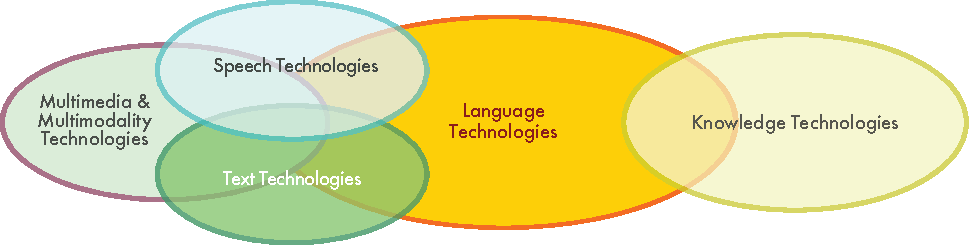
\includegraphics[width=\textwidth]{../_media/english/language_technologies}
  \caption{Language technology in context}
  \label{fig:ltincontext-eng}
  \colorrule{grey3}{\textwidth}{1.5pt}
\end{figure*}


In the following, we will discuss the main application areas of
language technology, i.\,e., language checking, web search, speech
technology, and machine translation. This includes
applications and basic technologies such as
\begin{itemize}
\item spelling correction

\item authoring support

\item computer-assisted language learning

\item information retrieval

\item information extraction

\item text summarisation

\item question answering

\item speech recognition

\item speech synthesis
\end{itemize}

Language technology is an established area of research with an extensive set of introductory literature. The interested reader is referred to the following references:  \cite{carstensen-etal1, jurafsky-martin01, manning-schuetze1, lt-world1, lt-survey1}.\\
Before discussing the above application areas, we will shortly
describe the architecture of a typical LT system.

\subsection{Application Architectures}

Software applications for language processing typically consist of
several components that mirror different aspects of language. 
While such applications tend to be very complex, figure~\ref{fig:textprocessingarch-eng} shows a highly simplified architecture of a typical text processing system. The first three modules handle the structure and meaning of the text input:

\begin{figure*}[b]
  \colorrule{grey3}{\textwidth}{1.5pt}
  \center
  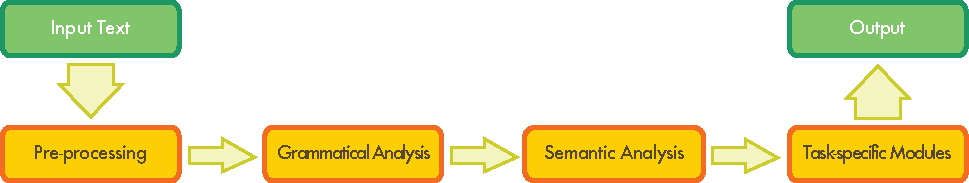
\includegraphics[width=\textwidth]{../_media/english/text_processing_app_architecture}
  \caption{A Typical Text Processing Architecture}
  \label{fig:textprocessingarch-eng}
  \colorrule{grey3}{\textwidth}{1.5pt}
\end{figure*}

\begin{enumerate}
\item Pre-processing: cleans the data, analyses or removes formatting,
detects the input language, and so on.

\item Grammatical analysis: finds the verb, its objects, modifiers and
other sentence elements; detects the sentence structure.

\item Semantic analysis: performs disambiguation (i.\,e., computes the
appropriate meaning of words in a given context); resolves anaphora
(i.\,e., which pronouns refer to which nouns in the sentence) and
substitute expressions; represents the meaning of the sentence in
a machine-readable way.
\end{enumerate}
After analysing the text, task-specific modules can perform other
operations, such as automatic summarisation and database
look-ups. \\
In the remainder of this section, we firstly introduce the core application areas for language technology, and follow this with a brief overview of the state of LT research and education today, and a description of past and present research programmes. Finally, we present an expert estimate of core LT tools and resources for Finnish in terms of various dimensions such as availability, maturity and quality. The general situation of LT for the Finnish language is summarised in a matrix (figure~\ref{fig:lrlttable_en}). 
LT support for German is also compared to other languages that are part of this series.


\subsection{Core Application Areas}

In this section, we focus on the most important LT tools and
resources, and give an overview of LT activities in Finland. 
Tools and resources that are boldfaced in the text can also be found in figure~\ref{fig:lrlttable_en} (p.~\pageref{fig:lrlttable_en}) at the end of this chapter. 


\subsubsection{Language Checking}

Anyone who has used a word processor knows that a spelling checker highlights 
spelling mistakes and proposes corrections.  The first spelling correction programs compared
a list of extracted words against a dictionary of correctly spelled
words. Today these programs are far more sophisticated. Using
language-dependent algorithms for \textbf{grammatical analysis},
they detect errors
related to morphology (e.\,g., plural formation) as well as
syntax–related errors, such as a missing verb or a conflict of
verb-subject agreement (e.\,g.,
\textit{\foreignlanguage{finnish}{\textit{me *kirjoittaa kirjeen}}}
 [a similar concept in English would be
\textit{she *write a letter}]).
But most spell checkers will not find any errors in the
following text:

\begin{quote}
  I have a spelling checker,\\
  It came with my PC.\\
  It plane lee marks four my revue\\
  Miss steaks aye can knot sea.~\cite{Surprise}
\end{quote}

Handling these kinds of errors usually requires an analysis of the
context. For example: if a word needs to be written in upper case in
Finnish or not:
\begin{itemize}
\item[] {\foreignlanguage{finnish}{\textit{Muista ottaa kaneli mukaan.}}} 
\item   {\textit{[Remember to take the cinnamon with you.]}}
\item[] {\foreignlanguage{finnish}{\textit{Muista ottaa Kaneli mukaan.}}}
\item   {\textit{[Remember to take Kaneli with you.]} }
\end{itemize}
This type of analysis either needs to draw on language-specific
\textbf{grammars} laboriously coded into the software by experts, or on a
statistical language model. In this case, a model calculates the
probability of a particular word as it occurs in a specific position
(e.\,g., between the words that precede and follow it). For example,
 {\foreignlanguage{finnish}{\textit{kaneli}}} is a much more probable
 as a noun than a proper noun
 {\foreignlanguage{finnish}{\textit{Kaneli}}}.
A statistical language model can be automatically created by using a
large amount of (correct) language data (called a \textbf{text corpus}).
Most
of these two approaches have been developed around data from
English. Neither approach can transfer easily to Finnish because the
language has a flexible word order, unlimited compound building and a
richer inflection system.

\begin{figure*}[t]
  \colorrule{grey3}{\textwidth}{1.5pt}
  \center
  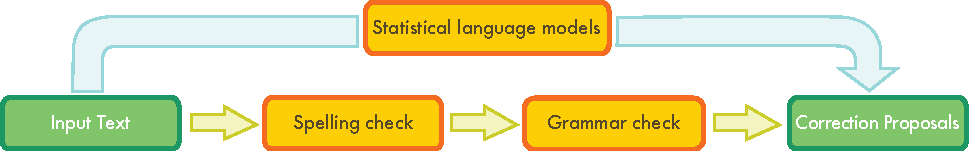
\includegraphics[width=\textwidth]{../_media/english/language_checking}
  \caption{Language checking (top: statistical; bottom: rule-based)}
  \label{fig:langcheckingarch-eng}
  \colorrule{grey3}{\textwidth}{1.5pt}
\end{figure*}

\boxtext{The use of language checking is not limited to word processors; it also applies to authoring support systems.}

Language checking is not limited to word processors; it is also used
in “authoring support systems”, i.\,e., software environments in which
manuals and other documentation are written to special standards for
complex IT, healthcare, engineering and other products. Fearing
customer complaints about incorrect use and damage claims resulting
from poorly understood instructions, companies are increasingly
focusing on the quality of technical documentation while targeting the
international market (via translation or localisation) at the same
time. Advances in natural language processing have led to the
development of authoring support software, which helps the writer of
technical documentation use vocabulary and sentence structures that
are consistent with industry rules and (corporate) terminology
restrictions.\\
Finnish has a history of several small Finnish companies and Language
Service Providers developing products based on various language
models. Finnish is a challenging language to model, or as Antti Arppe
put it in 2002: "Whereas in English one can in principle create a
prototypical language engineering tool such as a simple spell-checker
by merely listing and compressing the most common 100,000 words or so,
in Finnish one would need to list tens if not hundreds of millions of
word forms to create a speller with comparable coverage using the same
technique." \cite{NoPath} Since the late 1980's, there has been a
series of language proofing tools from available from Kielikone,
nowadays specializing in dictionaries, Connexor specializing in
language analysis tools, Gurusoft specializing in SOM-applications,
and Lingsoft offering a wide selection of tools,
including hyphenation and proofreading for Finnish.\\
Besides spell checkers and authoring support, language checking is
also important in the field of computer-assisted language
learning. And language checking applications also automatically
correct search engine queries, as found in Google's \textit{Did you
mean\dots} suggestions.

\subsubsection{Web Search}

Searching the Web, intranets or digital libraries is probably the
most widely used yet largely underdeveloped language technology
application today. The Google search engine, which started in 1998,
now handles about 80\% of all search queries \cite{spi1}. The verb
\textit{\foreignlanguage{finnish}{\textit{guuglata}}} is used in everyday
speech in Finnish although there is no conventional way to spell it
yet. The Google search interface and results page display has not
significantly changed since the first version. Yet in the current
version, Google offers spelling correction for misspelled words and
has now incorporated basic semantic search capabilities that can
improve search accuracy by analysing the meaning of terms in a search
query context \cite{Google-rolls}. The Google success story shows that
a large volume of available data and efficient indexing techniques can
deliver satisfactory results for a statistically-based approach.\\
For more sophisticated information requests, it is essential to
integrate deeper linguistic knowledge to \textbf{semantic
analysis}. Experiments using \textbf{lexical resources} such
as machine-readable thesauri or ontological language resources (e.\,g.,
WordNet for English or the equivalent Finnish FinnWordNet) have
demonstrated improvements in finding pages using synonyms of the
original search terms, such as
{\foreignlanguage{finnish}{\textit{atomienergia}}} \textit{[atomic energy]},
{\foreignlanguage{finnish}{\textit{ydinvoima}}} \textit{[atomic power]} and
{\foreignlanguage{finnish}{\textit{ydinenergia}}} \textit{[nuclear energy]},
or even more loosely related terms.

\begin{figure*}[htb]
  \colorrule{grey3}{\textwidth}{1.5pt}
  \center
  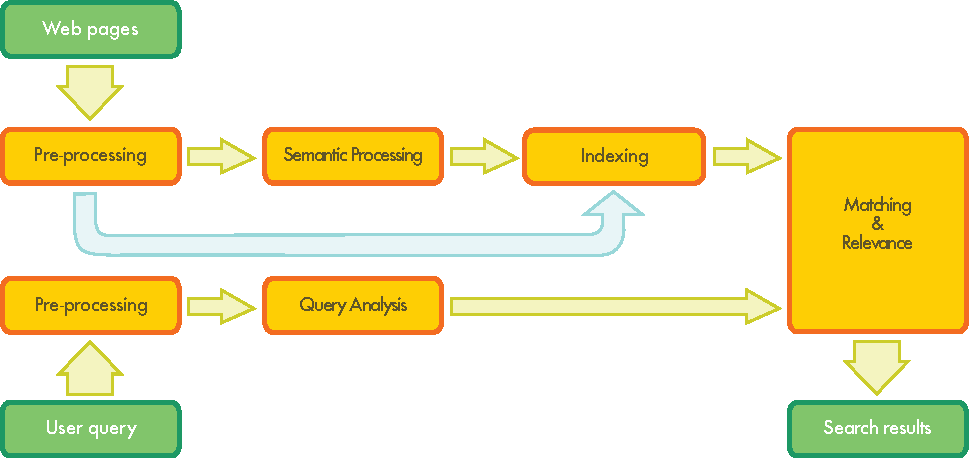
\includegraphics[width=\textwidth]{../_media/english/web_search_architecture}
  \caption{Web Search}
  \label{fig:websearcharch-eng}
  \colorrule{grey3}{\textwidth}{1.5pt}
 \end{figure*}

\boxtext{The next generation of search engines will have to include much more sophisticated language technology.}

The next generation of search engines will have to include much more
sophisticated language technology, in particular in order to deal with
search queries consisting of a question or other sentence type rather
than a list of keywords. For the query, “Give me a list of all
companies that were taken over by other companies in the last five
years,” the LT system needs to analyse the sentence syntactically and
semantically as well as provide an index to quickly retrieve relevant
documents. A satisfactory answer will require syntactic parsing to
analyse the grammatical structure of the sentence and determine that
the user wants companies that have been acquired, not companies that
acquired other companies. For the expression \textit{last five years},
the system needs to determine the relevant years. And, the query needs
to be matched against a huge amount of unstructured data to find the
piece or pieces of relevant information the user wants. This is called
“information retrieval”, and involves searching and ranking relevant
documents. To generate a list of companies, the system also needs to recognise a particular string of words in a document represents a company name, using a process called named entity recognition.\\
A more demanding challenge is matching a query in one language with
documents in another language. Cross-lingual information retrieval
involves automatically translating the query into all possible source
languages and then translating the results back into the user's target
language.\\
Now that data is increasingly found in non-textual formats, there is a
need for services that deliver multimedia information retrieval by
searching images, audio files and video data. In the case of audio and
video files, a speech recognition module must convert the speech
content into text (or into a phonetic representation) that can then be
matched against a user query.\\
In Finland, there are few small and medium size enterprises to actively develop and apply search
technologies at the moment, although Gurusoft specialises in applying
language independent Self-organizing maps (SOM methods) to information
retrieval tasks, but the product Docunaut is designed to apply the method in searches within the intranets of their customers instead of the world wide web. At present
there are no ongoing large-scale Finnish language search engine
projects.

\subsubsection{Speech Technology}

Speech interaction is one of many application areas that depend on speech technology, i.\,e., technologies for processing spoken language. Speech interaction technology is used to create interfaces that enable users to interact in spoken language instead of using a graphical display, keyboard and mouse.  \\
Today, these voice user interfaces (VUI) are used for partially or fully automated telephone services provided by companies to customers, employees or partners. Business domains that rely heavily on VUIs include banking, supply chain, public transportation, and telecommunications. Other uses of speech 
interaction
technology include interfaces to car navigation systems and the use of spoken language as an alternative to the graphical or touchscreen interfaces in smartphones.  
\boxtext{Speech technology is the basis for creating interfaces that allow a user to interact with spoken language instead of a graphical display, keyboard and mouse.}

Speech 
interaction
technology comprises four technologies:

\begin{enumerate}
\item Automatic \textbf{speech recognition} (ASR) determines which words are actually
    spoken in a given sequence of sounds uttered by a user.

\item Natural language understanding analyses the syntactic structure of a user’s
    utterance and interprets it according to the system in question.

\item Dialogue management determines which action to take given the user input
    and system functionality.

\item \textbf{Speech synthesis} (text-to-speech or TTS) transforms the system’s reply into
    sounds for the user.
\end{enumerate}

\begin{figure*}[htb]
  \colorrule{grey3}{\textwidth}{1.5pt}
  \center
  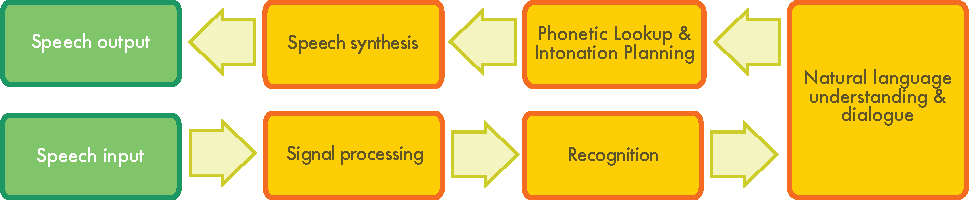
\includegraphics[width=\textwidth]{../_media/english/simple_speech-based_dialogue_architecture}
    \caption{Speech-based dialogue system}
    \label{fig:dialoguearch-eng}
    \colorrule{grey3}{\textwidth}{1.5pt}
  \end{figure*}

One of the major challenges of ASR systems is to accurately recognise the words
a user utters. This means restricting the range of possible user utterances to
a limited set of keywords, or manually creating language models that cover a
large range of natural language utterances. Using machine learning techniques,
language models can also be generated automatically from \textbf{speech corpora}, i.\,e.,
large collections of speech audio files and text transcriptions. Restricting
utterances usually forces people to use the voice user interface in a rigid way
and can damage user acceptance; but the creation, tuning and maintenance of
rich language models will significantly increase costs. VUIs that employ
language models and initially allow a user to express their intent more
flexibly — prompted by a \textit{How may I help you?} greeting — tend to be automated
and are better accepted by users.\\
Companies tend to use utterances pre-recorded by professional speakers for
generating the output of the voice user interface. For static utterances where
the wording does not depend on particular contexts of use or personal user
data, this can deliver a rich user experience. But more dynamic content in an
utterance may suffer from unnatural intonation because different parts of audio files have
simply been strung together. Today’s TTS systems are getting better (though
they can still be optimised) at producing natural-sounding dynamic utterances.\\
Interfaces in the market for speech technology 
have been considerably standardised during the last decade in terms of their various
technology components. There has also been strong market consolidation in
speech recognition and speech synthesis. The national markets in the G20
countries (economically resilient countries with high populations) have been
dominated by just five global players, with Nuance (USA) and Loquendo (Italy)
being the most prominent players in Europe. In 2011, Nuance announced the
acquisition of Loquendo, which represents a further step in market
consolidation.\\
Research in speech technology has been undertaken in Finland as early as the
1960s, with some results having an international renown or impact such as the
portable Synte 2 speech synthesizer, developed by the Acoustics Laboratory in
the 1970s and the phonetic typewriter in the 1980s, both developed at the
University of Technology (currently Aalto University). There have also been
some individual speech products on the market since the early 1990s; however,
their clientele have been limited mainly to special groups such as the visually
impaired. After the turn of the millennium a clear change has been witnessed.
Both the public and the private sectors have embarked on major research and
development projects in speech technology, which are starting to bear fruit -
there now exist several basic technological solutions for both speech
recognition and synthesis of Finnish that are on par with any language. Most
speech technology companies working on a global level offer both TTS and ASR
for Finnish. Two Finnish companies (Bitlips Oy and Timehouse Oy) offer Finnish
TTS. Bitlips also has English, Finland Swedish and Welsh synthesis. Lingsoft Oy
and Suomen Puheentunnistus Oy both have Finnish ASR systems and provide VUI
services for several Finnish corporations.\\
There are currently several major research projects on speech on both TTS and
ASR in Finland. The bulk of the research is done at Aalto University,
University of Helsinki, Tampere University of Technology. The main industrial
contributor to speech research in Finland has traditionally been Nokia.\\
Regarding dialogue management technology and know-how, there exist no SMEs
offering products in these areas. Finally, within the domain of Speech
Interaction, a genuine market for the linguistic core technologies for
syntactic and semantic analysis does not exist yet.\\
Looking ahead, there will be significant changes due to the spread of
smartphones as a new platform for managing customer relationships in addition
to fixed telephones, the Internet and e-mail. This will also affect how speech
technology is used. In the long run, there will be fewer
telephone-based VUIs and spoken language will play a far more central role as a
user-friendly input for smartphones. This will be largely driven by stepped
improvements in the accuracy of speaker-independent speech recognition via
speech dictation services already offered as centralised services to smartphone
users.

\subsubsection{Machine Translation}

The idea of using digital computers to translate natural languages goes back to
1946 and was followed by substantial funding for research during the 1950s and
again in the 1980s. Yet \textbf{machine translation} (MT) still cannot meet its initial
promise of across-the-board automated translation.

\boxtext{At its basic level, Machine Translation simply substitutes words in one natural language with words in another language.}
The most basic approach to machine translation is to automatically replace the
words in a text in one natural language by words in another language. This can
be useful in subject domains that have a very restricted, formulaic language
such as weather reports. But to produce a good translation of less standardised
texts, larger text units (phrases, sentences, or even whole passages) need to
be matched to their closest counterparts in the target language. The major
difficulty is that human language is ambiguous. Ambiguity creates challenges on
multiple levels, such as word sense disambiguation at the lexical level (a
\textit{jaguar} is a brand of car or an animal) or the assignment of case on the
syntactic level, for example:
\begin{itemize}
\item[] {\foreignlanguage{finnish}
         {\textit{Poliisi tarkkaili miestä mäellä.}}} 
\item        \textit{[The policeman observed the man on the hill.]}

\item[] {\foreignlanguage{finnish}{\textit{Poliisi tarkkaili miestä
                kiikarilla.}}} 
\item        \textit{[The policeman observed the man with binoculars.]}
\end{itemize}
One way to build an MT system is to use linguistic rules. For translations
between closely related languages, a direct substitution translation may be
feasible in cases like the above example. But, rule-based (or linguistic
knowledge-driven) systems often analyse the input text and create an
intermediary symbolic representation from which the text can be generated into
the target language. The success of these methods is highly dependent on the
availability of extensive lexicons with morphological, syntactic, and semantic
information, and large sets of grammar rules carefully designed by skilled
linguists. This is a very long and therefore costly process.\\
In the late 1980s when computational power increased and became cheaper, there
was more interest in statistical models for machine translation. Statistical
models are derived from analysing bilingual text corpora, such as the Europarl
\textbf{parallel corpus}, which contains the proceedings of the European Parliament in
21 European languages. Given enough data, statistical MT works well enough to
derive an approximate meaning of a foreign language text by processing parallel
versions and finding plausible patterns of words. But unlike knowledge-driven
systems, statistical (or data-driven) MT often generates ungrammatical output.
Data-driven MT is advantageous because less human effort is required, and it
can also cover special particularities of the language (e.\,g., idiomatic
expressions) that can get ignored in knowledge-driven systems.

\begin{figure*}[htb]
  \colorrule{grey3}{\textwidth}{1.5pt}
  \center
  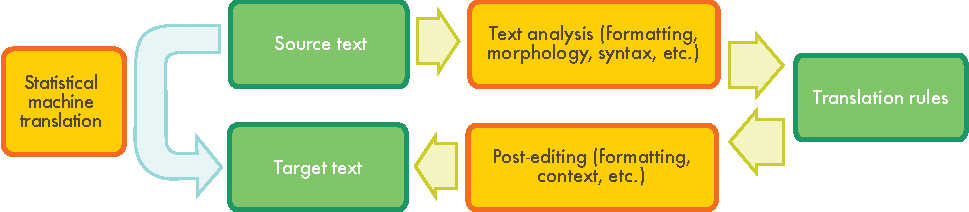
\includegraphics[width=\textwidth]{../_media/english/machine_translation}
  \caption{Machine translation (left: statistical; right: rule-based)}
  \label{fig:mtarch-eng}
  \colorrule{grey3}{\textwidth}{1.5pt}
\end{figure*}

The strengths and weaknesses of knowledge-driven and data-driven machine
translation tend to be complementary, so that nowadays researchers focus on
hybrid approaches that combine both methodologies. One approach uses both
knowledge-driven and data-driven systems together with a selection module that
decides on the best output for each sentence. However, results for sentences
longer than say 12 words will often be far from perfect. A better solution is
to combine the best parts of each sentence from multiple outputs; this can be
fairly complex, as corresponding parts of multiple alternatives are not always
obvious and need to be aligned.

\boxtext{Machine Translation is particularly challenging for the Finnish language.}
Finland missed out on first generation machine translation, but caught the
second wave of rule-based machine translation in the 80’s. A long-term
nationally funded R\&D project Kielikone first developed the necessary Finnish
analysis tools and used them to build a rule-based Finnish-to-English MT system
in the 90’s that subsequently became a commercial product. IBM Finland
researched English-to-Finnish transfer based on the IBM English parser at the
turn of the 90’s but did not reach product stage. Sunda, a newer rule based
system developed from the Kielikone technology base, now sells relatively good
quality English-to-Finnish MT. Google and Microsoft provide statistical MT for
Finnish, but the quality remains poor, due to the complexity of Finnish
morphology and the free word order which current statistical MT is poorly
equipped for. The technical university has a group working on statistical
language modelling of Finnish, including Finnish morphology and SMT.\\
There is still a huge potential for improving the quality of MT
systems. The challenges involve adapting language resources to a given
subject domain or user area, and integrating the technology into
workflows that already have term bases and translation
memories. Another problem is that most of the current systems are
English-centred and only support a few languages from and into
Finnish. This leads to friction in the translation workflow and forces
MT users to learn different lexicon coding tools for different
systems.\\
Evaluation campaigns help compare the quality of MT systems, the
different approaches and the status of the systems for different
language pairs. Figure \ref{fig:euromatrix} (page
\pageref{fig:euromatrix}), which was prepared during the EC
Euromatrix+ project, shows the pair-wise performances obtained for 22
of the 23 official EU languages. (Irish was not compared.). The
results are ranked according to a BLEU score, which indicates higher
scores for better translations \cite{BLEU}. A human translator would
achieve a score of around 80 points.\\
The best results (in green and blue) were achieved by languages that
benefit from a considerable research effort in coordinated programs
and from the existence of many parallel corpora (e.\,g., English,
French, Dutch, Spanish and German). The languages with poorer results
are shown in red. These languages either lack such development efforts
or are structurally very different from other languages (e.\,g.,
Hungarian, Maltese and Finnish).


\subsection{Other Application Areas}

Building language technology applications involves a range of subtasks that do
not always surface at the level of interaction with the user, but they provide
significant service functionalities “under the hood” of the system in question.
They all form important research issues that have now evolved into individual
sub-disciplines of computational linguistics.
\boxtext{Language technology applications often provide significant service functionalities “under the hood” of larger software systems.}

Question answering, for example, is an active area of research for which
annotated corpora have been built and scientific competitions have been
initiated. The concept of question answering goes beyond keyword-based searches
(in which the search engine responds by delivering a collection of potentially
relevant documents) and enables users to ask a concrete question to which the
system provides a single answer. For example:
\begin{itemize}
\item[] \textit{Question: How old was Neil Armstrong when he stepped on the
              moon?}

\item[] \textit{Answer: 38.}
\end{itemize}
While question answering is obviously related to the core area of web search,
it is nowadays an umbrella term for such research issues as what different
types of questions there are, and how they should be handled; how a set of
documents that potentially contain the answer can be analysed and compared (do
they provide conflicting answers?); and how specific information (the answer)
can be reliably extracted from a document without ignoring the context.\\
Question answering is in turn related to information extraction (IE), an area that was
extremely popular and influential when computational linguistics took a
statistical turn in the early 1990s. IE aims to identify specific pieces of
information in specific classes of documents, such as detecting the key players
in company takeovers as reported in newspaper stories. Another common scenario
that has been studied is reports on terrorist incidents. The problem here is to
map the text to a template that specifies the perpetrator, target, time,
location and results of the incident. Domain-specific template-filling is the
central characteristic of IE, which makes it another example of a “behind the
scenes” technology that forms a well-demarcated research area that in practice
needs to be embedded into a suitable application environment.

\boxtext{For the Finnish language, research in most text technologies is much less developed than for the English language.}

Text summarisation and \textbf{text generation} are two borderline areas that can act
either as standalone applications or play a supporting role “under the hood”.
Summarisation attempts to give the essentials of a long text in a short form,
and is one of the features available in Microsoft Word. It mostly uses a
statistical approach to identify the “important” words in a text (i.\,e., words
that occur very frequently in the text in question but less frequently in
general language use) and determine which sentences contain the most of these
“important” words. These sentences are then extracted and put together to
create the summary. In this very common commercial scenario, summarisation is
simply a form of sentence extraction, and the text is reduced to a subset of
its sentences. An alternative approach, for which some research has been
carried out, is to generate brand new sentences that do not exist in the source
text. This requires a deeper understanding of the text, which means that so far
this approach is far less robust. On the whole, a text generator is rarely used
as a stand-alone application but is embedded into a larger software
environment, such as a clinical information system that collects, stores and
processes patient data. Creating reports is just one of many applications for
text summarisation.\\
For the Finnish language, research in these text technologies is much
less developed than for the English language. Question answering,
information extraction, and summarisation have been the focus of
numerous open competitions in the USA since the 1990s, primarily
organised by the government-sponsored organisations DARPA and
NIST. These competitions have significantly improved the
start-of-the-art, but their focus has mostly been on the English
language.  As a result, there are hardly any annotated corpora or
other special resources needed to perform these tasks in Finnish. When
summarisation systems use purely statistical methods, they are largely
language-independent and a number of research prototypes are
available. For text generation, reusable components have traditionally
been limited to surface realisation modules (generation grammars) and
most of the available software is for the English language.  


\subsection{Educational Programmes}

Language technology is a very interdisciplinary field that involves the combined expertise of linguists, computer scientists, mathematicians, philosophers, psycholinguists, and neuroscientists among others. 
Language Technology has been
taught as a major subject at the University of Helsinki since 1994, and it has
been active in cooperation with other universities offering courses in the
neighbouring fields on both national and international level. The national
level includes the establishment of KIT Network for Language Technology Studies
in 2001 with 10 universities all over Finland participating in course exchange
and a common syllabus. The formal agreement between the universities ended in
2007 but the students enrolled in Finnish universities can apply for a grant
from their faculties to take Language Technology courses within the network.
The KIT Network universities include Aalto University, University of Eastern
Finland, University of Helsinki, University of Jyväskylä, University of Tampere, Technical University of
Tampere, University of Turku, University of Vaasa, University of Oulu, and Åbo
Akademi in Turku.\\
During 2006 - 2009 the students with a sufficient knowledge in Language
Technology could, after completing their BA, apply for a special master's
degree in Language Technology at the University of Helsinki. The master's
degree programme offered an option to focus on language technology, speech
technology or translation studies as a major. In 2009 the formal Master's
degree programme came to end with the new organisation structures taking place,
and it is now possible to apply to study advanced studies offered by the
language technology subject towards an MA in language technology.\\
The Graduate School of Language Technology in Finland (the KIT Graduate School)
was a multidisciplinary national graduate school, functioning during t2004 -
2009 as part of the emerging network of graduate schools of language technology
in the Nordic countries, Nordic Graduate School of Language Technology, NGSLT.
The KIT Graduate School was granted five PhD student positions for two
four-year periods 2002 - 2005 and 2006 - 2009. From the beginning of 2010 the
graduate school merged with LANGNET, the Finnish doctoral programme in language
studies, and became one of its programmes.\\
The education of language technology researchers in sufficient numbers
is nevertheless a prerequisite for the diverse research and thus the
development of successful commercial activity \cite{FinExp}.

\subsection{National Projects and Efforts}

The most important agencies for research funding in Finland are
the Academy of Finland financed by the Ministry of Education and
Culture and the Finnish Funding Agency for Technology and Innovation
(Tekes) financed by the Ministry of Trade and Industry \cite{Leading}.
Sitra, The Finnish National Fund for Research and Development had
provided funding for the MT project Kielikone in the 1980's Public
support from TEKES has been an important source of funding for basic
research especially through two large technology programs, USIX
(User-Oriented Information Technology) 1999 – 2002 and FENIX
(Interactive Computing) 2003 – 2007.\\
The USIX technology program aimed at raising the needs of the users and the
consumers of products and technologies by providing Finnish enterprises and
research institutions with funding for improving the quality of the products
and technologies. Some of the core technologies identified in the program were
Finnish speech recognition, large data management and search interfaces. The
program financed 181 projects with the total volume of 84 MEUR (44 MEUR
provided by Tekes) of which 29\% were research projects. Examples of NLP USIX
projects are WEBSOM developing Self-Organizing Map (SOM) technologies and GILTA
on Managing Large Text Masses, INTERACT, STT Speech-to-Text (research and
development of the phonemic speech recognition for Finnish), the joint project
for Finnish speech technology SuoPuhe, Noise Robust Multilingual Speech
Recognition, Dictionaries and language checking tools, and Multilingual
adaptative translation knowledge base, led jointly by most Finnish universities
and several enterprises. Several commercial products developed within the USIX
framework are available in the market today \cite{LoppuUSIX}.\\
The NLP projects carried out within the FENIX technology program include FENIX
4M (Mobile and Multilingual Maintenance Man) and FinnONTO (Semantic Web
Ontologies) at the University of Helsinki, New methods and applications in
speech processing and Search-in-a-Box (University of Turku), Rich semantic
media for personal and professional users (VTT Technical Research Centre of
Finland) and Intelligent Web Services (Helsinki School of Science and
Technology), StatHouse Semantics and Automatic content classification and
ontologies (Seerco Ltd) \cite{FinalFENIX}.\\
Recently, A joint project on speech synthesis between the University of
Helsinki and Aalto University has been very successful in the new field of
statistical parametric synthesis based on Hidden Markov Models and a new,
physiologically grounded vocoding technology. Developing speech synthesis is
very data oriented.\\
EU funded projects in Finland since the 1980’s include LR SIMPLE, LR
PAROLE and EU MLIS 5008 LINGMACHINE.  The Common Language Resources
and Technologies Infrastructure (CLARIN) was funded by the Commission
during 2008 – 2010, and the work within the initiative continues. The
national part FIN-CLARIN is funded by the Ministry of Education and
Culture. The FIN-CLARIN consortium comprises the following partners:
IT Center for Science CSC, The Institute for the Languages of
Finland KOTUS, the universities of Helsinki, Eastern Finland,
Jyväskylä, Oulu, Tampere, Turku, Vaasa, Aalto University and Åbo
Akademi. HFST (Helsinki Finite State Transducer Technology), OMor
(Open Source Morphologies), FinnWordNet, and FinnTreeBank are examples
of currently ongoing projects.\\
Language Technology at the University of Helsinki also cooperated in 2000 –
2004 on an international level in several projects within the
\textit{Språgteknologiprogram} (Nordic Language Technology Research Program)
funded by
the Nordic Council of Ministers. The Finnish Language Technology documentation
centre FiLT was established to promote availability of language technology
resources, both for commercial and academic players.\\
As we have seen, previous programmes have led to the development of a number of
LT tools and resources for the Finnish language. In the following section, the
current state of LT support for Finnish is summarised.

\subsection{Availability of Tools and Resources}

Table \ref{fig:lrlttable_en} summarises the current state of language
technology support for the Finnish language. The rating for existing
tools and resources was generated by leading experts in the field who
provided estimates based on a scale from 0 (very low) to 6 (very high)
according to seven criteria.

\begin{figure*}[htb]
\centering
\begin{tabular}{>{\columncolor{orange1}}p{.33\linewidth}@{\hspace*{6mm}}c@{\hspace*{6mm}}c@{\hspace*{6mm}}c@{\hspace*{6mm}}c@{\hspace*{6mm}}c@{\hspace*{6mm}}c@{\hspace*{6mm}}c}
\rowcolor{orange1}
 \cellcolor{white}&\begin{sideways}\makecell[l]{Quantity}\end{sideways}
&\begin{sideways}\makecell[l]{\makecell[l]{Availability} }\end{sideways} &\begin{sideways}\makecell[l]{Quality}\end{sideways}
&\begin{sideways}\makecell[l]{Coverage}\end{sideways} &\begin{sideways}\makecell[l]{Maturity}\end{sideways} &\begin{sideways}\makecell[l]{Sustainability~~}\end{sideways} &\begin{sideways}\makecell[l]{Adaptability}\end{sideways} \\ \addlinespace
\multicolumn{8}{>{\columncolor{orange2}}l}{Language Technology: Tools, Technologies and Applications} \\ \addlinespace
Speech Recognition	& 3 & 2 & 4 & 3 & 3 & 3 & 4  \\ \addlinespace
Speech Synthesis & 3 & 3 & 5 & 4 & 4 & 4 & 4\\ \addlinespace
Grammatical analysis & 3,5 & 3,5 & 3,5 & 4 & 4 & 3,5 & 3,5\\ \addlinespace
Semantic analysis & 0,4 & 0,4 & 1 & 1 & 1 & 1,4 & 0,7\\ \addlinespace
Text generation & 3 & 3 & 4 & 2 & 3 & 3 & 4\\ \addlinespace
Machine translation & 3 & 1 & 4 & 2 & 3 & 1 & 2\\ \addlinespace
\multicolumn{8}{>{\columncolor{orange2}}l}{Language Resources: Resources, Data and Knowledge Bases} \\ \addlinespace
Text corpora & 3 & 4 & 4 & 3,5 & 3,5 & 3,5 & 4\\ \addlinespace
Speech corpora & 2 & 3 & 3 & 2 & 2 & 2 & 2\\ \addlinespace
Parallel corpora & 1 & 2 & 3 & 2 & 2 & 3 & 3\\ \addlinespace
Lexical resources & 3 & 4 & 3,5 & 4 & 3,5 & 3,5 & 3,5\\ \addlinespace
Grammars & 2 & 5 & 4 & 4 & 4 & 3 & 3\\
\end{tabular}
\caption{State of language technology support for Finnish}
\label{fig:lrlttable_en}
\end{figure*}

The key results for the Finnish language can be summed up as follows:
\begin{itemize}
\item While some specific corpora of high quality exist, sufficiently large
    syntactically annotated corpora are not available yet and many of the
    resources lack standardisation. The commercial sector in Finland needs
    large, up-to date resources for the product development targeted to the big
    public.

\item There are several tools for syntactical analysis available based on various
    linguistic models. In general, they work well given the particularities of
    the Finnish language. Work on semantics has not led to applications yet.

\item In Speech technology, the biggest leap forward in Finland has been taken in
    the area of speech recognition. Due to the particularities of Finnish, the
    word lists or lexicons required for speech recognition have been
    impractically large. A speech technology research group at the Helsinki
    University of Technology (Aalto university) presented already in 2002 a method for automated
    word segmentation that enabled reducing the size of the lexicon
    dramatically. This breakthrough has not yet been implemented in the
    commercial sector. Speech synthesis research has moved forward considerably
    during the last few years. However, the work is still in the laboratory
    phase, and considerable resources are needed to bring the system to the
    market. Speech corpora are hard to collect and require a lot of work.

\item There are only very few projects working on information retrieval for
    Finnish. It is more usual to take an existing tool and implement a Finnish
    stemmer as part of it leading to licensing and limited rights to use the
    tool in other environments.

\item There are few multimodal resources and virtually no advanced discourse
    processing tools available for Finnish.

\item An unclear legal situation restricts making use of digital texts, such as
    those published online by newspapers, for empirical linguistic and language
    technology research, for example, to train statistical language models.
    Together with politicians and policy makers, researchers should try to
    establish laws or regulations that enable researchers to use publicly
    available texts for language-related R\&D activities.
\end{itemize}

To conclude, in a number of specific areas of Finnish language research, we
have software with limited functionality available today. Obviously, further
research efforts are required to meet the current deficit in processing texts
on a deeper semantic level and to address the lack of resources such as
parallel corpora for machine translation.

\subsection{Cross-language comparison}

The current state of LT support varies considerably from one language
community to another. In order to compare the situation between
languages, this section will present an evaluation based on two sample
application areas (machine translation and speech processing) and one
underlying technology (text analysis), as well as basic resources
needed for building LT applications.

The languages were categorised using the following five-point scale: 

\begin{enumerate}
\item Excellent support
\item Good support
\item Moderate support
\item Fragmentary support
\item Weak or no support
\end{enumerate}

Language Technology support was measured according to the following criteria:
\begin{itemize}
\item Speech Processing: Quality of existing speech recognition
       technologies, quality of existing speech synthesis
       technologies, coverage of domains, number and size of existing
       speech corpora, amount and variety of available speech-based
       applications
\item Machine Translation: Quality of existing MT technologies, number
       of language pairs covered, coverage of linguistic phenomena and
       domains, quality and size of existing parallel corpora, amount
       and variety of available MT applications

\item Text Analysis: Quality and coverage of existing text analysis
       technologies (morphology, syntax, semantics), coverage of
       linguistic phenomena and domains, amount and variety of
       available applications, quality and size of existing
       (annotated) text corpora, quality and coverage of existing
       lexical resources (e.\,g., WordNet) and grammars
\item Resources: Quality and size of existing text corpora, speech
       corpora and parallel corpora, quality and coverage of existing
       lexical resources and grammars
\end{itemize}

Figures~\ref{fig:speech_cluster_en} to~\ref{fig:resources_cluster_en} (p.~\pageref{fig:speech_cluster_en} and~\pageref{fig:resources_cluster_en}) show that the LT funding and thus the resources available for
developing resources for the Finnish language in the recent decades has been
smaller than for the major European languages in general, and particularly
English. Based on the evaluation, machine translation technologies for Finnish
have been classified to the cluster of low support. For speech processing,
current technologies perform well enough to be successfully integrated into a
number of industrial applications such as spoken dialogue and dictation
systems, especially for special languages. The need for language resources both
for text and speech technologies is evident. Text analysis components already
cover the linguistic phenomena of Finnish to a certain extent and form part of
many applications, e.\,g. spelling correction and function on a satisfactory
level.\\
For building more sophisticated applications, such as machine translation,
there is a clear need for resources and technologies that cover a wider range
of linguistic aspects and allow a deep semantic analysis of the input text. By
improving the quality and coverage of these basic resources and technologies,
we shall be able to open up new opportunities for tackling a vast range of
advanced application areas, including high-quality machine translation.

\subsection{Conclusions}

\emph{In this series of white papers, we have made an important effort by assessing the language technology support for 30 European languages, and by providing a high-level comparison across these languages. By identifying the gaps, needs and deficits, the European language technology community and its related stakeholders are now in a position to design a large scale research and development programme aimed at building a truly multilingual, technology-enabled communication across Europe.}

We have seen that there are huge differences between Europe’s
languages. While there are good quality software and resources
available for some languages and application areas, others (usually
‘smaller’ languages) have substantial gaps.  Many languages lack basic
technologies for text analysis and the essential resources for
developing these technologies. Others have basic tools and resources
but are as yet unable to invest in semantic processing. We therefore
still need to make a large-scale effort to attain the ambitious goal
of providing high-quality machine translation between all European
languages.\\
Basic research in language technology was well funded in the 1980's
and 1990's but since then the funding has been less satisfying. Even
if some language technology development projects received funding in
the 2000's from the leading Finnish funding agencies, the Finnish
Funding Agency for Technology and Innovation (Tekes) and the Academy
of Finland, the results and material developed in these projects have
not been widely and openly distributed. As the present report shows,
the situation in language technology is acceptable only for the most
basic tools and resources. Finland is lagging behind in the
development of essential digital resources necessary for the survival
of a language as defined in the BLARK (Basic Language Resource Kit)
for speech, text and lexicons. The BLARK is essential in developing
the language technology modules for creating language technology
tools. There is a growing demand for large-scale up-to-date resources
for the language technology research and product development for the
benefit of the Finnish society.\\
Current efforts within the large-scale European research
infrastructure project Common Language Re-sources and Technologies
Infrastructure (CLARIN) and in the Multilingual Europe Technology
Alliance (META) aim at supporting language resource and technology
distribution and access on a European level. However, the national
needs in Finland have not yet been adequately addressed.\\
Our findings show that the only alternative is to make a substantial
effort to create LT resources for Finnish, and use them to drive
forward research, innovation and development. The need for large
amounts of data and the extreme complexity of language technology
systems makes it vital to develop a new infrastructure and a more
coherent research organisation to spur greater sharing and
cooperation.\\
There is also a lack of continuity in research and development
funding.  Short-term coordinated programmes tend to alternate with
periods of sparse or zero funding. We can therefore conclude that
there is a desperate need for a large, coordinated initiative focused
on overcoming the differences in language technology readiness for
European languages as a whole.\\
META-NET’s long-term goal is to introduce high-quality language
technology for all languages in order to achieve political and
economic unity through cultural diversity. The technology will help
tear down existing barriers and build bridges between Europe’s
languages. This requires all stakeholders - in politics, research,
business, and society - to unite their efforts for the future.

\end{multicols}


\clearpage

\begin{figure*}[t]
  \small
  \centering
  \begin{tabular}
  { % defines color for each column.
  >{\columncolor{corange5}}p{.13\linewidth}@{\hspace{.040\linewidth}}
  >{\columncolor{corange4}}p{.13\linewidth}@{\hspace{.040\linewidth}}
  >{\columncolor{corange3}}p{.13\linewidth}@{\hspace{.040\linewidth}}
  >{\columncolor{corange2}}p{.13\linewidth}@{\hspace{.040\linewidth}}
  >{\columncolor{corange1}}p{.13\linewidth} 
  }
  \multicolumn{1}{>{\columncolor{white}}c@{\hspace{.040\linewidth}}}{\textbf{Excellent}} & 
  \multicolumn{1}{@{}>{\columncolor{white}}c@{\hspace{.040\linewidth}}}{\textbf{Good}} &
  \multicolumn{1}{@{}>{\columncolor{white}}c@{\hspace{.040\linewidth}}}{\textbf{Moderate}} &
  \multicolumn{1}{@{}>{\columncolor{white}}c@{\hspace{.040\linewidth}}}{\textbf{Fragmentary}} &
  \multicolumn{1}{@{}>{\columncolor{white}}c}{\textbf{Weak/no}} \\ 
  \multicolumn{1}{>{\columncolor{white}}c@{\hspace{.040\linewidth}}}{\textbf{support}} & 
  \multicolumn{1}{@{}>{\columncolor{white}}c@{\hspace{.040\linewidth}}}{\textbf{support}} &
  \multicolumn{1}{@{}>{\columncolor{white}}c@{\hspace{.040\linewidth}}}{\textbf{support}} &
  \multicolumn{1}{@{}>{\columncolor{white}}c@{\hspace{.040\linewidth}}}{\textbf{support}} &
  \multicolumn{1}{@{}>{\columncolor{white}}c}{\textbf{support}} \\ \addlinespace
  
& \vspace*{0.5mm}English
& \vspace*{0.5mm}
Czech \newline 
Dutch \newline 
\textbf{Finnish} \newline 
French \newline 
German \newline   
Italian \newline  
Portuguese \newline 
Spanish \newline
& \vspace*{0.5mm}Basque \newline 
Bulgarian \newline 
Catalan \newline 
Danish \newline 
Estonian \newline 
Galician\newline 
Greek \newline  
Hungarian  \newline
Irish \newline  
Norwegian \newline 
Polish \newline 
Serbian \newline 
Slovak \newline 
Slovene \newline 
Swedish \newline
& \vspace*{0.5mm}
Croatian \newline 
Icelandic \newline  
Latvian \newline 
Lithuanian \newline 
Maltese \newline 
Romanian\\
\end{tabular}
\caption{Speech processing: state of language technology support for 30 European languages}
\label{fig:speech_cluster_en}
\end{figure*}

\begin{figure*}[b]
  \small
  \centering
  \begin{tabular}
  { % defines color for each column.
  >{\columncolor{corange5}}p{.13\linewidth}@{\hspace{.040\linewidth}}
  >{\columncolor{corange4}}p{.13\linewidth}@{\hspace{.040\linewidth}}
  >{\columncolor{corange3}}p{.13\linewidth}@{\hspace{.040\linewidth}}
  >{\columncolor{corange2}}p{.13\linewidth}@{\hspace{.040\linewidth}}
  >{\columncolor{corange1}}p{.13\linewidth} 
  }
  \multicolumn{1}{>{\columncolor{white}}c@{\hspace{.040\linewidth}}}{\textbf{Excellent}} & 
  \multicolumn{1}{@{}>{\columncolor{white}}c@{\hspace{.040\linewidth}}}{\textbf{Good}} &
  \multicolumn{1}{@{}>{\columncolor{white}}c@{\hspace{.040\linewidth}}}{\textbf{Moderate}} &
  \multicolumn{1}{@{}>{\columncolor{white}}c@{\hspace{.040\linewidth}}}{\textbf{Fragmentary}} &
  \multicolumn{1}{@{}>{\columncolor{white}}c}{\textbf{Weak/no}} \\ 
  \multicolumn{1}{>{\columncolor{white}}c@{\hspace{.040\linewidth}}}{\textbf{support}} & 
  \multicolumn{1}{@{}>{\columncolor{white}}c@{\hspace{.040\linewidth}}}{\textbf{support}} &
  \multicolumn{1}{@{}>{\columncolor{white}}c@{\hspace{.040\linewidth}}}{\textbf{support}} &
  \multicolumn{1}{@{}>{\columncolor{white}}c@{\hspace{.040\linewidth}}}{\textbf{support}} &
  \multicolumn{1}{@{}>{\columncolor{white}}c}{\textbf{support}} \\ \addlinespace
  
& \vspace*{0.5mm} English 
& \vspace*{0.5mm} 
French \newline 
Spanish
& \vspace*{0.5mm}
Catalan \newline 
Dutch \newline 
German \newline 
Hungarian \newline
Italian \newline 
Polish \newline 
Romanian \newline 
& \vspace*{0.5mm}Basque \newline 
Bulgarian \newline 
Croatian \newline 
Czech \newline
Danish \newline 
Estonian \newline 
\textbf{Finnish} \newline 
Galician \newline 
Greek \newline 
Icelandic \newline 
Irish \newline 
Latvian \newline 
Lithuanian \newline 
Maltese \newline 
Norwegian \newline 
Portuguese \newline 
Serbian \newline 
Slovak \newline 
Slovene \newline 
Swedish \newline 
\end{tabular}
\caption{Machine translation: state of language technology support for 30 European languages}
\label{fig:mt_cluster_en}
\end{figure*}

\begin{figure*}[t]
  \small
  \centering
  \begin{tabular}
  { % defines color for each column.
  >{\columncolor{corange5}}p{.13\linewidth}@{\hspace{.040\linewidth}}
  >{\columncolor{corange4}}p{.13\linewidth}@{\hspace{.040\linewidth}}
  >{\columncolor{corange3}}p{.13\linewidth}@{\hspace{.040\linewidth}}
  >{\columncolor{corange2}}p{.13\linewidth}@{\hspace{.040\linewidth}}
  >{\columncolor{corange1}}p{.13\linewidth} 
  }
  \multicolumn{1}{>{\columncolor{white}}c@{\hspace{.040\linewidth}}}{\textbf{Excellent}} & 
  \multicolumn{1}{@{}>{\columncolor{white}}c@{\hspace{.040\linewidth}}}{\textbf{Good}} &
  \multicolumn{1}{@{}>{\columncolor{white}}c@{\hspace{.040\linewidth}}}{\textbf{Moderate}} &
  \multicolumn{1}{@{}>{\columncolor{white}}c@{\hspace{.040\linewidth}}}{\textbf{Fragmentary}} &
  \multicolumn{1}{@{}>{\columncolor{white}}c}{\textbf{Weak/no}} \\ 
  \multicolumn{1}{>{\columncolor{white}}c@{\hspace{.040\linewidth}}}{\textbf{support}} & 
  \multicolumn{1}{@{}>{\columncolor{white}}c@{\hspace{.040\linewidth}}}{\textbf{support}} &
  \multicolumn{1}{@{}>{\columncolor{white}}c@{\hspace{.040\linewidth}}}{\textbf{support}} &
  \multicolumn{1}{@{}>{\columncolor{white}}c@{\hspace{.040\linewidth}}}{\textbf{support}} &
  \multicolumn{1}{@{}>{\columncolor{white}}c}{\textbf{support}} \\ \addlinespace

& \vspace*{0.5mm}English
& \vspace*{0.5mm}
  Dutch \newline 
  French \newline 
  German \newline 
  Italian \newline 
  Spanish
& \vspace*{0.5mm}Basque \newline 
  Bulgarian \newline 
  Catalan \newline 
  Czech \newline 
  Danish \newline 
  \textbf{Finnish} \newline 
  Galician \newline 
  Greek \newline 
  Hungarian \newline 
  Norwegian \newline 
  Polish \newline 
  Portuguese \newline 
  Romanian \newline 
  Slovak \newline 
  Slovene \newline 
  Swedish \newline 
& \vspace*{0.5mm}
  Croatian \newline 
  Estonian \newline 
  Icelandic \newline 
  Irish \newline 
  Latvian \newline 
  Lithuanian \newline 
  Maltese \newline 
  Serbian \\
  \end{tabular}
\caption{Text analysis: state of language technology support for 30 European languages}
\label{fig:text_cluster_en}
\end{figure*}

\begin{figure*}[b]
  \small
  \centering
  \begin{tabular}
  { % defines color for each column.
  >{\columncolor{corange5}}p{.13\linewidth}@{\hspace{.040\linewidth}}
  >{\columncolor{corange4}}p{.13\linewidth}@{\hspace{.040\linewidth}}
  >{\columncolor{corange3}}p{.13\linewidth}@{\hspace{.040\linewidth}}
  >{\columncolor{corange2}}p{.13\linewidth}@{\hspace{.040\linewidth}}
  >{\columncolor{corange1}}p{.13\linewidth} 
  }
  \multicolumn{1}{>{\columncolor{white}}c@{\hspace{.040\linewidth}}}{\textbf{Excellent}} & 
  \multicolumn{1}{@{}>{\columncolor{white}}c@{\hspace{.040\linewidth}}}{\textbf{Good}} &
  \multicolumn{1}{@{}>{\columncolor{white}}c@{\hspace{.040\linewidth}}}{\textbf{Moderate}} &
  \multicolumn{1}{@{}>{\columncolor{white}}c@{\hspace{.040\linewidth}}}{\textbf{Fragmentary}} &
  \multicolumn{1}{@{}>{\columncolor{white}}c}{\textbf{Weak/no}} \\ 
  \multicolumn{1}{>{\columncolor{white}}c@{\hspace{.040\linewidth}}}{\textbf{support}} & 
  \multicolumn{1}{@{}>{\columncolor{white}}c@{\hspace{.040\linewidth}}}{\textbf{support}} &
  \multicolumn{1}{@{}>{\columncolor{white}}c@{\hspace{.040\linewidth}}}{\textbf{support}} &
  \multicolumn{1}{@{}>{\columncolor{white}}c@{\hspace{.040\linewidth}}}{\textbf{support}} &
  \multicolumn{1}{@{}>{\columncolor{white}}c}{\textbf{support}} \\ \addlinespace
    
& \vspace*{0.5mm}
    English
& \vspace*{0.5mm} 
    Czech \newline 
    Dutch \newline 
    French \newline 
    German \newline 
    Hungarian \newline
    Italian \newline
    Polish \newline
    Spanish \newline
    Swedish \newline 
& \vspace*{0.5mm}
    Basque\newline 
    Bulgarian\newline 
    Catalan \newline 
    Croatian \newline 
    Danish \newline 
    Estonian \newline 
    \textbf{Finnish} \newline 
    Galician \newline 
    Greek \newline 
    Norwegian \newline 
    Portuguese \newline 
    Romanian \newline 
    Serbian \newline 
    Slovak \newline 
    Slovene \newline
&  \vspace*{0.5mm}
    Icelandic \newline 
    Irish \newline 
    Latvian \newline 
    Lithuanian \newline 
    Maltese  \\
  \end{tabular}
  \caption{Speech and text resources: state of support for 30 European languages}  
  \label{fig:resources_cluster_en}
\end{figure*}

\cleardoublepage
%_-----------------------------------------
\ssection[About META-NET]{About META-NET}
\begin{multicols}{2}

META-NET is a Network of Excellence funded by the European
Commission. The network currently consists of 54 members from 33
European countries~\cite{rehm2011}. META-NET fosters the Multilingual Europe
Technology Alliance (META), a growing community of language technology
professionals and organisations in Europe.

% Figger: Countries Represented in META-NET

META-NET cooperates with other initiatives like the Common Language
Resources and Technology Infrastructure (CLARIN), which is helping to
establish digital humanities research in Europe. META-NET fosters the
technological foundations for a truly multilingual European
information society that:
\begin{itemize}
\item makes communication and cooperation possible across languages;

\item provides equal access to information and knowledge in any language;

\item offers advanced and affordable networked information technology to European
    citizens.
\end{itemize}
META-NET stimulates and promotes multilingual technologies for all
European languages. The technologies enable automatic translation,
content production, information processing and knowledge management
for a wide variety of applications and subject domains. The network
wants to improve current approaches, so better communication and
cooperation across languages can take place. Europeans have an equal
right to information and knowledge regardless of language.

META-NET launched on 1 February 2010 with the goal of advancing
research in language technology (LT). The network supports a Europe
that unites as a single digital market and information space. META-NET
has conducted several activities that further its goals. META-VISION,
META-SHARE and META-RESEARCH are the network’s three lines of action.

% Fig: Three Lines of Action in META-NET

\textbf{META-VISION} fosters a dynamic and influential stakeholder
community that unites around a shared vision and a common strategic
research agenda (SRA). The main focus of this activity is to build a
coherent and cohesive LT community in Europe by bringing together
representatives from highly fragmented and diverse groups of
stakeholders. In the first year of META-NET, presentations at the
FLaReNet Forum (Spain), Language Technology Days (Luxembourg),
JIAMCATT 2010 (Luxembourg), LREC 2010 (Malta), EAMT 2010 (France) and
ICT 2010 (Belgium) centred on public outreach. According to initial
estimates, META-NET has already contacted more than 2,500 LT
professionals to develop its goals and visions with them. At the
META-FORUM 2010 event in Brussels, META-NET communicated the initial
results of its vision building process to more than 250
participants. In a series of interactive sessions, the participants
provided feedback on the visions presented by the network.

\textbf{META-SHARE} creates an open, distributed facility for
exchanging and sharing resources. The peer-to-peer network of
repositories will contain language data, tools and web services that
are documented with high-quality metadata and organised in
standardised categories. The resources can be readily accessed and
uniformly searched. The available resources include free, open source
materials as well as restricted, commercially available, fee-based
items. META-SHARE targets existing language data, tools and systems as
well as new and emerging products that are required for building and
evaluating new technologies, products and services. The reuse,
combination, repurposing and re-engineering of language data and tools
plays a crucial role. META-SHARE will eventually become a critical
part of the LT marketplace for developers, localisation experts,
researchers, translators and language professionals from small,
mid-sized and large enterprises. META-SHARE addresses the full
development cycle of LT—from research to innovative products and
services. A key aspect of this activity is establishing META-SHARE as
an important and valuable part of a European and global infrastructure
for the LT community.

\textbf{META-RESEARCH} builds bridges to related technology
fields. This activity seeks to leverage advances in other fields and
to capitalise on innovative research that can benefit language
technology. In particular, this activity wants to bring more semantics
into machine translation (MT), optimise the division of labour in
hybrid MT, exploit context when computing automatic translations and
prepare an empirical base for MT. META-RESEARCH is working with other
fields and disciplines, such as machine learning and the Semantic Web
community.  META-RESEARCH focuses on collecting data, preparing data
sets and organising language resources for evaluation purposes;
compiling inventories of tools and methods; and organising workshops
and training events for members of the community. This activity has
already clearly identified aspects of MT where semantics can impact
current best practices. In addition, the activity has created
recommendations on how to approach the problem of integrating semantic
information into MT. META-RESEARCH is also finalising a new language
resource for MT, the Annotated Hybrid Sample MT Corpus, which provides
data for English-German, English-Spanish and English-Czech language
pairs. META-RESEARCH has also developed software that collects
multilingual corpora that are hidden on the Web.
\end{multicols}

\vfill
\centerline{office@meta-net.eu -- http://www.meta-net.eu}

\cleardoublepage

\appendix
\addtocontents{toc}{\protect\bigskip}

\bsection[Viitteet -- References]{Viitteet --- References}
\bibliographystyle{unsrt}
\bibliography{finnish_references}
  
\cleardoublepage

%\bsection{Jäsenet -- Members}
\bsection[META-NET Jäsenet -- META-NET Members]{META-NET Jäsenet --- META-NET Members}
\label{metanetmembers}

%Taulukossa esitellään META-NET –verkostoon osallistuvat
%tutkimuslaitokset ja niiden edustajat.

\small

\begin{longtable}{@{}llp{113mm}@{}}
Alankomaat & \textcolor{grey1}{Netherlands} & Utrecht Institute of Linguistics, Utrecht University: Jan Odijk\\ \addlinespace 
  & & Computational Linguistics, University of Groningen: Gertjan van Noord\\ \addlinespace
Belgia & \textcolor{grey1}{Belgium} & Computational Linguistics and Psycholinguistics Research Centre, University of Antwerp: Walter Daelemans\\ \addlinespace
  & & Centre for Processing Speech and Images, University of Leuven: Dirk van Compernolle \\ \addlinespace
Bulgaria & \textcolor{grey1}{Bulgaria} & Institute for Bulgarian Language, Bulgarian Academy of Sciences: Svetla Koeva \\ \addlinespace
Espanja & \textcolor{grey1}{Spain} & Barcelona Media: Toni Badia, Maite Melero \\ \addlinespace 
  & & Institut Universitari de Lingüística Aplicada, Universitat Pompeu Fabra: Núria Bel \\ \addlinespace 
  & & Aholab Signal Processing Laboratory, University of the Basque Country:\newline Inma Hernaez Rioja \\ \addlinespace 
  & & Center for Language and Speech Technologies and Applications, Universitat Politècnica de Catalunya:  Asunción Moreno \\ \addlinespace 
  & & Department of Signal Processing and Communications, University of Vigo:\newline Carmen García Mateo \\ \addlinespace 
Irlanti & \textcolor{grey1}{Ireland} & School of Computing, Dublin City University: Josef van Genabith\\ \addlinespace
Islanti & \textcolor{grey1}{Iceland} & School of Humanities, University of Iceland: Eiríkur Rögnvaldsson\\ \addlinespace
Itävalta & \textcolor{grey1}{Austria} & Zentrum für Translationswissenschaft, Universität Wien: Gerhard Budin\\ \addlinespace 
Italia & \textcolor{grey1}{Italy} & Consiglio Nazionale delle Ricerche, Istituto di Linguistica Computazionale “Antonio Zampolli”: Nicoletta Calzolari\\ \addlinespace
  & & Human Language Technology Research Unit, Fondazione Bruno Kessler:\newline Bernardo Magnini\\ \addlinespace 
Kreikka & \textcolor{grey1}{Greece} & R.C. “Athena”, Institute for Language and Speech Processing: Stelios Piperidis\\ \addlinespace
Kroatia & \textcolor{grey1}{Croatia} & Institute of Linguistics, Faculty of Humanities and Social Science, University of Zagreb: Marko Tadić \\ \addlinespace
Kypros & \textcolor{grey1}{Cyprus} & Language Centre, School of Humanities: Jack Burston\\ \addlinespace
Latvia & \textcolor{grey1}{Latvia} & Tilde: Andrejs Vasiļjevs\\ \addlinespace 
  & & Institute of Mathematics and Computer Science, University of Latvia: Inguna Skadiņa\\ \addlinespace
Liettua & \textcolor{grey1}{Lithuania} & Institute of the Lithuanian Language: Jolanta Zabarskaitė\\ \addlinespace
Luxembourg & \textcolor{grey1}{Luxembourg} & Arax Ltd.: Vartkes Goetcherian\\ \addlinespace
Malta & \textcolor{grey1}{Malta} & Department Intelligent Computer Systems, University of Malta: Mike Rosner\\ \addlinespace
Norja & \textcolor{grey1}{Norway} & Department of Linguistic, University of Bergen: Koenraad De Smedt\\ \addlinespace 
  & & Department of Informatics, Language Technology Group, University of Oslo:\newline Stephan Oepen \\ \addlinespace
Portugali & \textcolor{grey1}{Portugal} & University of Lisbon: António Branco, Amália Mendes \\ \addlinespace
  & & Spoken Language Systems Laboratory, Institute for Systems Engineering and Computers: Isabel Trancoso \\ \addlinespace
Puola & \textcolor{grey1}{Poland} & Institute of Computer Science, Polish Academy of Sciences: Adam Przepiórkowski, Maciej Ogrodniczuk \\ \addlinespace
  & & University of Łódź: Barbara Lewandowska-Tomaszczyk, Piotr Pęzik\\ \addlinespace
  & & Department of Computer Linguistics and Artificial Intelligence, Adam Mickiewicz University: Zygmunt Vetulani \\ \addlinespace
Ranska & \textcolor{grey1}{France} & Centre National de la Recherche Scientifique, Laboratoire d'Informatique pour la Mécanique et les Sciences de l'Ingénieur: Joseph Mariani \\ \addlinespace
  & & Evaluations and Language Resources Distribution Agency: Khalid Choukri\\ \addlinespace 
Romania & \textcolor{grey1}{Romania} & Research Institute for Artificial Intelligence, Romanian Academy of Sciences:\newline Dan Tufiș \\ \addlinespace
  & & Faculty of Computer Science, University Alexandru Ioan Cuza of Iași: Dan Cristea \\ \addlinespace
Ruotsi & \textcolor{grey1}{Sweden} & Department of Swedish, University of Gothenburg: Lars Borin \\ \addlinespace 
Saksa & \textcolor{grey1}{Germany} & Language Technology Lab, DFKI: Hans Uszkoreit, Georg Rehm\\ \addlinespace
  & & Human Language Technology and Pattern Recognition, RWTH Aachen University: Hermann Ney \\ \addlinespace
  & & Department of Computational Linguistics, Saarland University: Manfred Pinkal\\ \addlinespace 
Serbia & \textcolor{grey1}{Serbia} & University of Belgrade, Faculty of Mathematics: Duško Vitas, Cvetana Krstev,\newline Ivan Obradović \\ \addlinespace
  & & Pupin Institute: Sanja Vranes \\ \addlinespace  
Slovakia & \textcolor{grey1}{Slovakia} & Ľudovít Štúr Institute of Linguistics, Slovak Academy of Sciences: Radovan Garabík \\ \addlinespace 
Slovenia & \textcolor{grey1}{Slovenia} & Jožef Stefan Institute: Marko Grobelnik \\ \addlinespace 
Suomi & \textcolor{grey1}{Finland} & Computational Cognitive Systems Research Group, Aalto University: Timo Honkela\\ \addlinespace
& & Department of Modern Languages, University of Helsinki: Kimmo Koskenniemi, Krister Lindén \\ \addlinespace
Sveitsi & \textcolor{grey1}{Switzerland} & Idiap Research Institute: Hervé Bourlard \\ \addlinespace 
Tanska &  \textcolor{grey1}{Denmark} & Centre for Language Technology, University of Copenhagen: \newline Bolette Sandford Pedersen, Bente Maegaard\\ \addlinespace
Tšekin tasavalta & \textcolor{grey1}{Czech Republic} & Institute of Formal and Applied Linguistics, Charles University in Prague: Jan Hajič \\ \addlinespace
Unkari & \textcolor{grey1}{Hungary} & Research Institute for Linguistics, Hungarian Academy of Sciences: Tamás Váradi\\  \addlinespace
  & & Department of Telecommunications and Media Informatics, Budapest University of Technology and Economics: Géza Németh, Gábor Olaszy\\ \addlinespace
Viro & \textcolor{grey1}{Estonia} & Institute of Computer Science, University of Tartu: Tiit Roosmaa, Kadri Vider\\ \addlinespace
Britannia & \textcolor{grey1}{UK} & 
  School of Computer Science, University of Manchester: Sophia Ananiadou \\ \addlinespace 
  & & Institute for Language, Cognition and Computation, Center for Speech Technology Research, University of Edinburgh: Steve Renals \\ \addlinespace 
  & & Research Institute of Informatics and Language Processing, University of Wolverhampton: Ruslan Mitkov
\end{longtable}
\normalsize


\renewcommand*{\figureformat}{}
\renewcommand*{\captionformat}{}

\begin{figure*}[htbp]
  \colorrule{grey3}{\textwidth}{1.5pt}
  \center
  %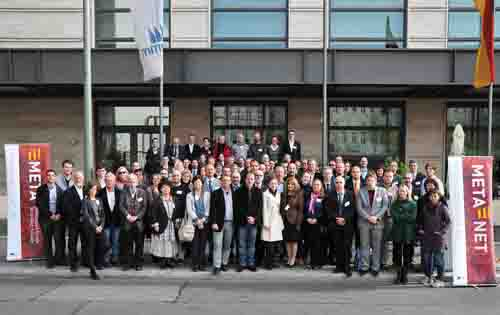
\includegraphics[width=\textwidth]{../_media/meta-net_team.jpg}
  \fbox{Dummy -- we'll include the group photo of our META-NET meeting in Berlin here}
  \caption{Lähes 100 kieliteknologian asiantuntijaa, jotka edustavat META-NET -hankkeen
jäsenmaita ja kansallisia kieliä,  viimeistelivät META-NET valkoisten kirjojen
julkaisusarjan keskeiset tulokset ja sanoman META-NET -hankkeen Berliinissä,
Saksassa pidetyssä kokouksessa 21-22.10.2011. --- \textcolor{grey1}{About 100 language technology experts -- representatives of the countries and languages represented in META-NET -- discussed and finalised the key results and messages of the White Paper Series at a META-NET meeting in Berlin, Germany, on October 21/22, 2011.}}
  \medskip
  \colorrule{grey3}{\textwidth}{1.5pt}
\end{figure*}

\cleardoublepage

\bsection[META-NET valkoiset kirjat -- The META-NET White Paper
Series]{META-NET\ \ \ \ \ \  valkoiset kirjat --- The META-NET\ \ \ \ \ \ White Paper Series}
\label{whitepaperseries}

\vspace*{-5mm}
\centering
  \setlength{\tabcolsep}{2.4em}
  \begin{tabularx}{\textwidth}{lllll} \toprule\addlinespace
&baski & Basque & euskara\\
&bulgaria & Bulgarian & български\\
&englanti & English & English\\
&espanja & Spanish & español\\
 &galicia & Galician & galego\\
 &hollanti & Dutch & Nederlands\\
 &iiri & Irish & Gaeilge\\
 &islanti & Icelandic & íslenska\\
 &italia & Italian & italiano\\
 &katalaani & Catalan & català\\
 &kreikka & Greek & ελληνικά\\
 &kroatia & Croatian & hrvatski\\
 &latvia & Latvian & latviešu valoda\\
 &liettua & Lithuanian & lietuvių kalba\\
 &malta & Maltese & Malti\\
 &norjan bokmål & Norwegian Bokmål & bokmål\\
 &norjan nynorsk & Norwegian Nynorsk & nynorsk\\
 &puola & Polish & polski\\
 &portugali & Portuguese & português\\
 &ranska & French & français\\
 &romania & Romanian & română\\
 &ruotsi & Swedish & svenska\\
 &saksa & German & Deutsch\\
 &serbia & Serbian & српски\\
 &slovakki & Slovak & slovenčina\\
 &sloveeni & Slovene & slovenščina\\
 &suomi & Finnish & suomi\\
 &tanska & Danish & dansk\\
 &tšekki & Czech & čeština\\
 &unkari & Hungarian & magyar\\
 &viro & Estonian & eesti\\
\addlinespace \bottomrule
\end{tabularx}

\end{document}
